\documentclass[12pt,twoside]{ctexart} 

\usepackage{fancyhdr} % Add this line
\usepackage{enumitem} % Add this line
\usepackage{caption} % Add this line
\usepackage{xcolor} % Add this line
\usepackage{titlesec} % Add this line

\setlength{\headheight}{12.64723pt} % Adjust headheight


\usepackage{ctex}
\usepackage{mdframed}
\usepackage{listings}
\usepackage{amsmath}
\usepackage{amssymb}
\usepackage{amsfonts}
\usepackage{graphicx}
\usepackage{subfigure}
\usepackage{float}
\usepackage{geometry}
\usepackage{fancyhdr}
\usepackage{lastpage} % Add this line
\usepackage{setspace}
\usepackage{rotating}
\usepackage[hidelinks]{hyperref}
\usepackage{booktabs}
\usepackage{siunitx}
\usepackage{cleveref}
\usepackage{microtype}
\usepackage{enumitem} % Add this line
\usepackage{caption} % Add this line
\usepackage{xcolor} % Add this line
\usepackage{titlesec} % Add this line

\lstset{
    basicstyle=\ttfamily\small,
    keywordstyle=\color{blue},
    stringstyle=\color{red},
    commentstyle=\color{green},
    morecomment=[l][\color{magenta}]{\#},
    breaklines=true,
    tabsize=4,
    showstringspaces=false,
    frame=single,
    numbers=left, % 在左侧显示行号
    numberstyle=\tiny\color{gray}, % 设置行号的样式
    captionpos=b, % 设置标题位置在底部
    abovecaptionskip=1em, % 设置标题上方的空白
    belowcaptionskip=1em, % 设置标题下方的空白
}

\doublespacing

\title{\Huge{\textbf{\fangsong 图书管理系统}}}
\author{\songti 无35 \\ 2023010625 \\ 黄皓宇}
\date{\today}

\pagestyle{fancy}
\fancyhf{} % 清除默认的页眉页脚
\lhead{图书管理系统}
\chead{\rightmark} % 使用\rightmark显示当前小节标题
\rhead{
\includegraphics[width=0.5cm]{logo0.jpg}} % 将姓名替换为logo
\lfoot{}
\cfoot{\thepage/\pageref{LastPage}} % 显示当前页码/总页码
\rfoot{}

\begin{document}

\begin{titlepage}
    \newgeometry{left=3cm,right=3cm,top=3cm,bottom=2.5cm} % Adjust page margins

    \centering % Center everything on the page

    \vspace*{2cm} % Add some vertical space at the top

    {\Huge\textbf{\heiti 图书管理系统}\par} % Title

    \vspace{0.5cm} % Add some vertical space

    {\large\textbf{用户指南}\par} % << Add this line for the course name

    \vspace{1.5cm} % Add some vertical space

    {\Large\textit{黄皓宇}\par} % Author name

    \vspace{0.5cm} % Add some vertical space

    {\large 无35\par} % Class

    \vspace{0.5cm} % Add some vertical space

    {\large 2023010625\par} % Student number

    \vspace{0.5cm} % Add flexible vertical space in the middle

    \begin{figure}[H]
        \centering
        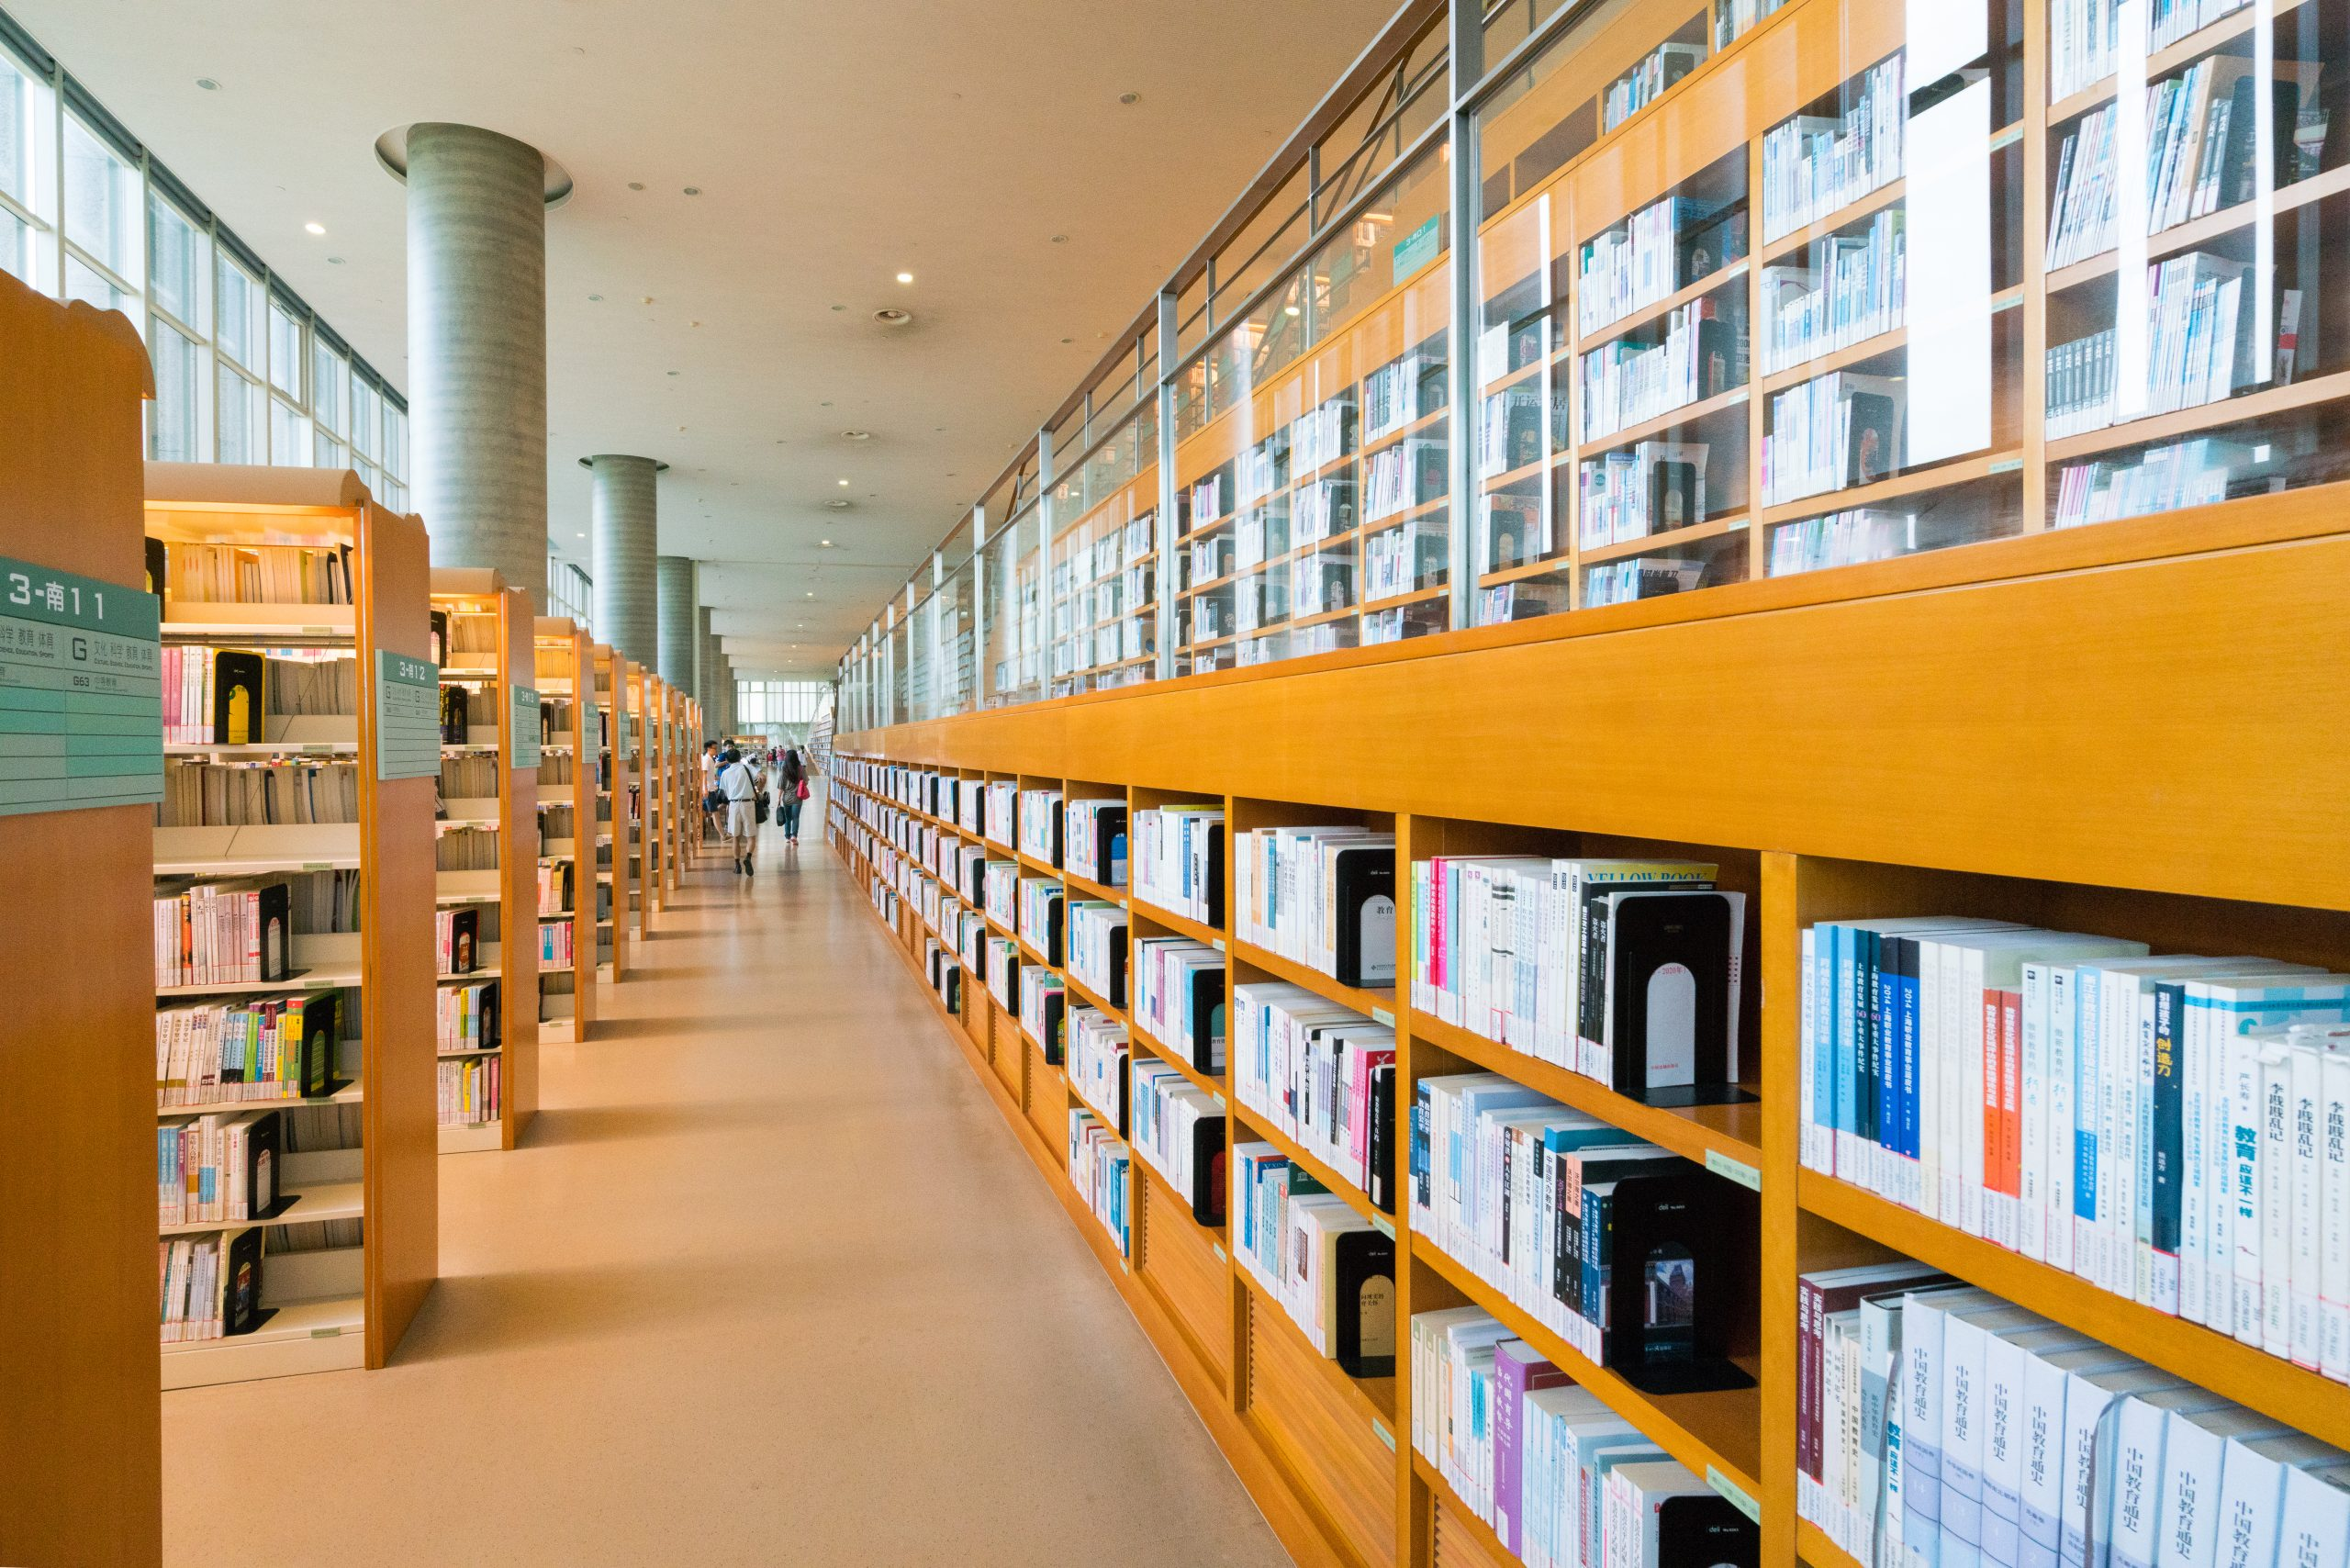
\includegraphics[width=0.8\textwidth]{System.jpg}
    \end{figure}



    {\large \today\par} % Date

    \restoregeometry % Restore the original page margins
\end{titlepage}

\setcounter{page}{0}
\pagenumbering{gobble} % 禁止显示页码
\thispagestyle{empty} % 确保此页不显示页码和页眉

\begin{center}
    \vspace*{\fill} % 垂直居中内容
    {\large
        \begin{tabular}{ll}
            文档标题 & 用户指南   \\
            版本号  & 1.2.0  \\
            发布日期 & \today \\
            文档状态 & 已校对    \\
            编写人员 & 黄皓宇    \\
        \end{tabular}
    }

\end{center}

\vspace*{\fill} % 垂直居中内容

\vspace{4cm} % 在底部信息和版权声明之间添加一些垂直空间
{\small 本文档中的信息(包括 URL 及其他 Internet 网站参考资料)可能随时变更,
    恕不另行通知。使用本文档的全部风险或因此导致的后果均由用户自行承担。除非另外注明,否则此处作为例子提到的公司、组织、产品、域名、电子邮件地址、
    徽标、人员、地点和时间纯属虚构,绝不意指,
    也不应由此臆测任何真实的公司、组织、产品、域名、电子邮件地址、徽标、人员、
    地点和时间。\par}




\newpage
% 恢复页码计数和显示
\setcounter{page}{1}
\pagenumbering{arabic}

\tableofcontents
\newpage

\section{产品概述}
\subsection{开发背景}
随着社会的发展,图书管理系统已经成为图书馆管理的重要工具。
图书管理系统是一种用于管理图书馆的软件系统,
它可以帮助图书馆管理人员更好地管理图书馆的图书、读者等信息,
提高图书馆的管理效率。图书管理系统可以帮助图书馆管理人员
更好地管理图书馆的图书、读者等信息,提高图书馆的管理效率。
图书管理系统可以帮助图书馆管理人员更好地管理图书馆的图书、读者等信息,
提高图书馆的管理效率。

\subsection{产品概述}
本系统是一个基于C++编写的图书管理系统,主要功能包括:
\begin{itemize}
    \item 用户信息管理:包括用户的姓名、联系方式、借阅数量、借阅历史等信息。
    \item 访客信息管理:包括访客的姓名、联系方式、访问次数等信息。
    \item 管理员信息管理:包括管理员的姓名、联系方式、管理权限等信息。
    \item 图书信息管理:包括图书的书名、作者、类别、关键字、简介、ISBN、价格等信息。

\end{itemize}

\begin{figure}[H]
    \centering
    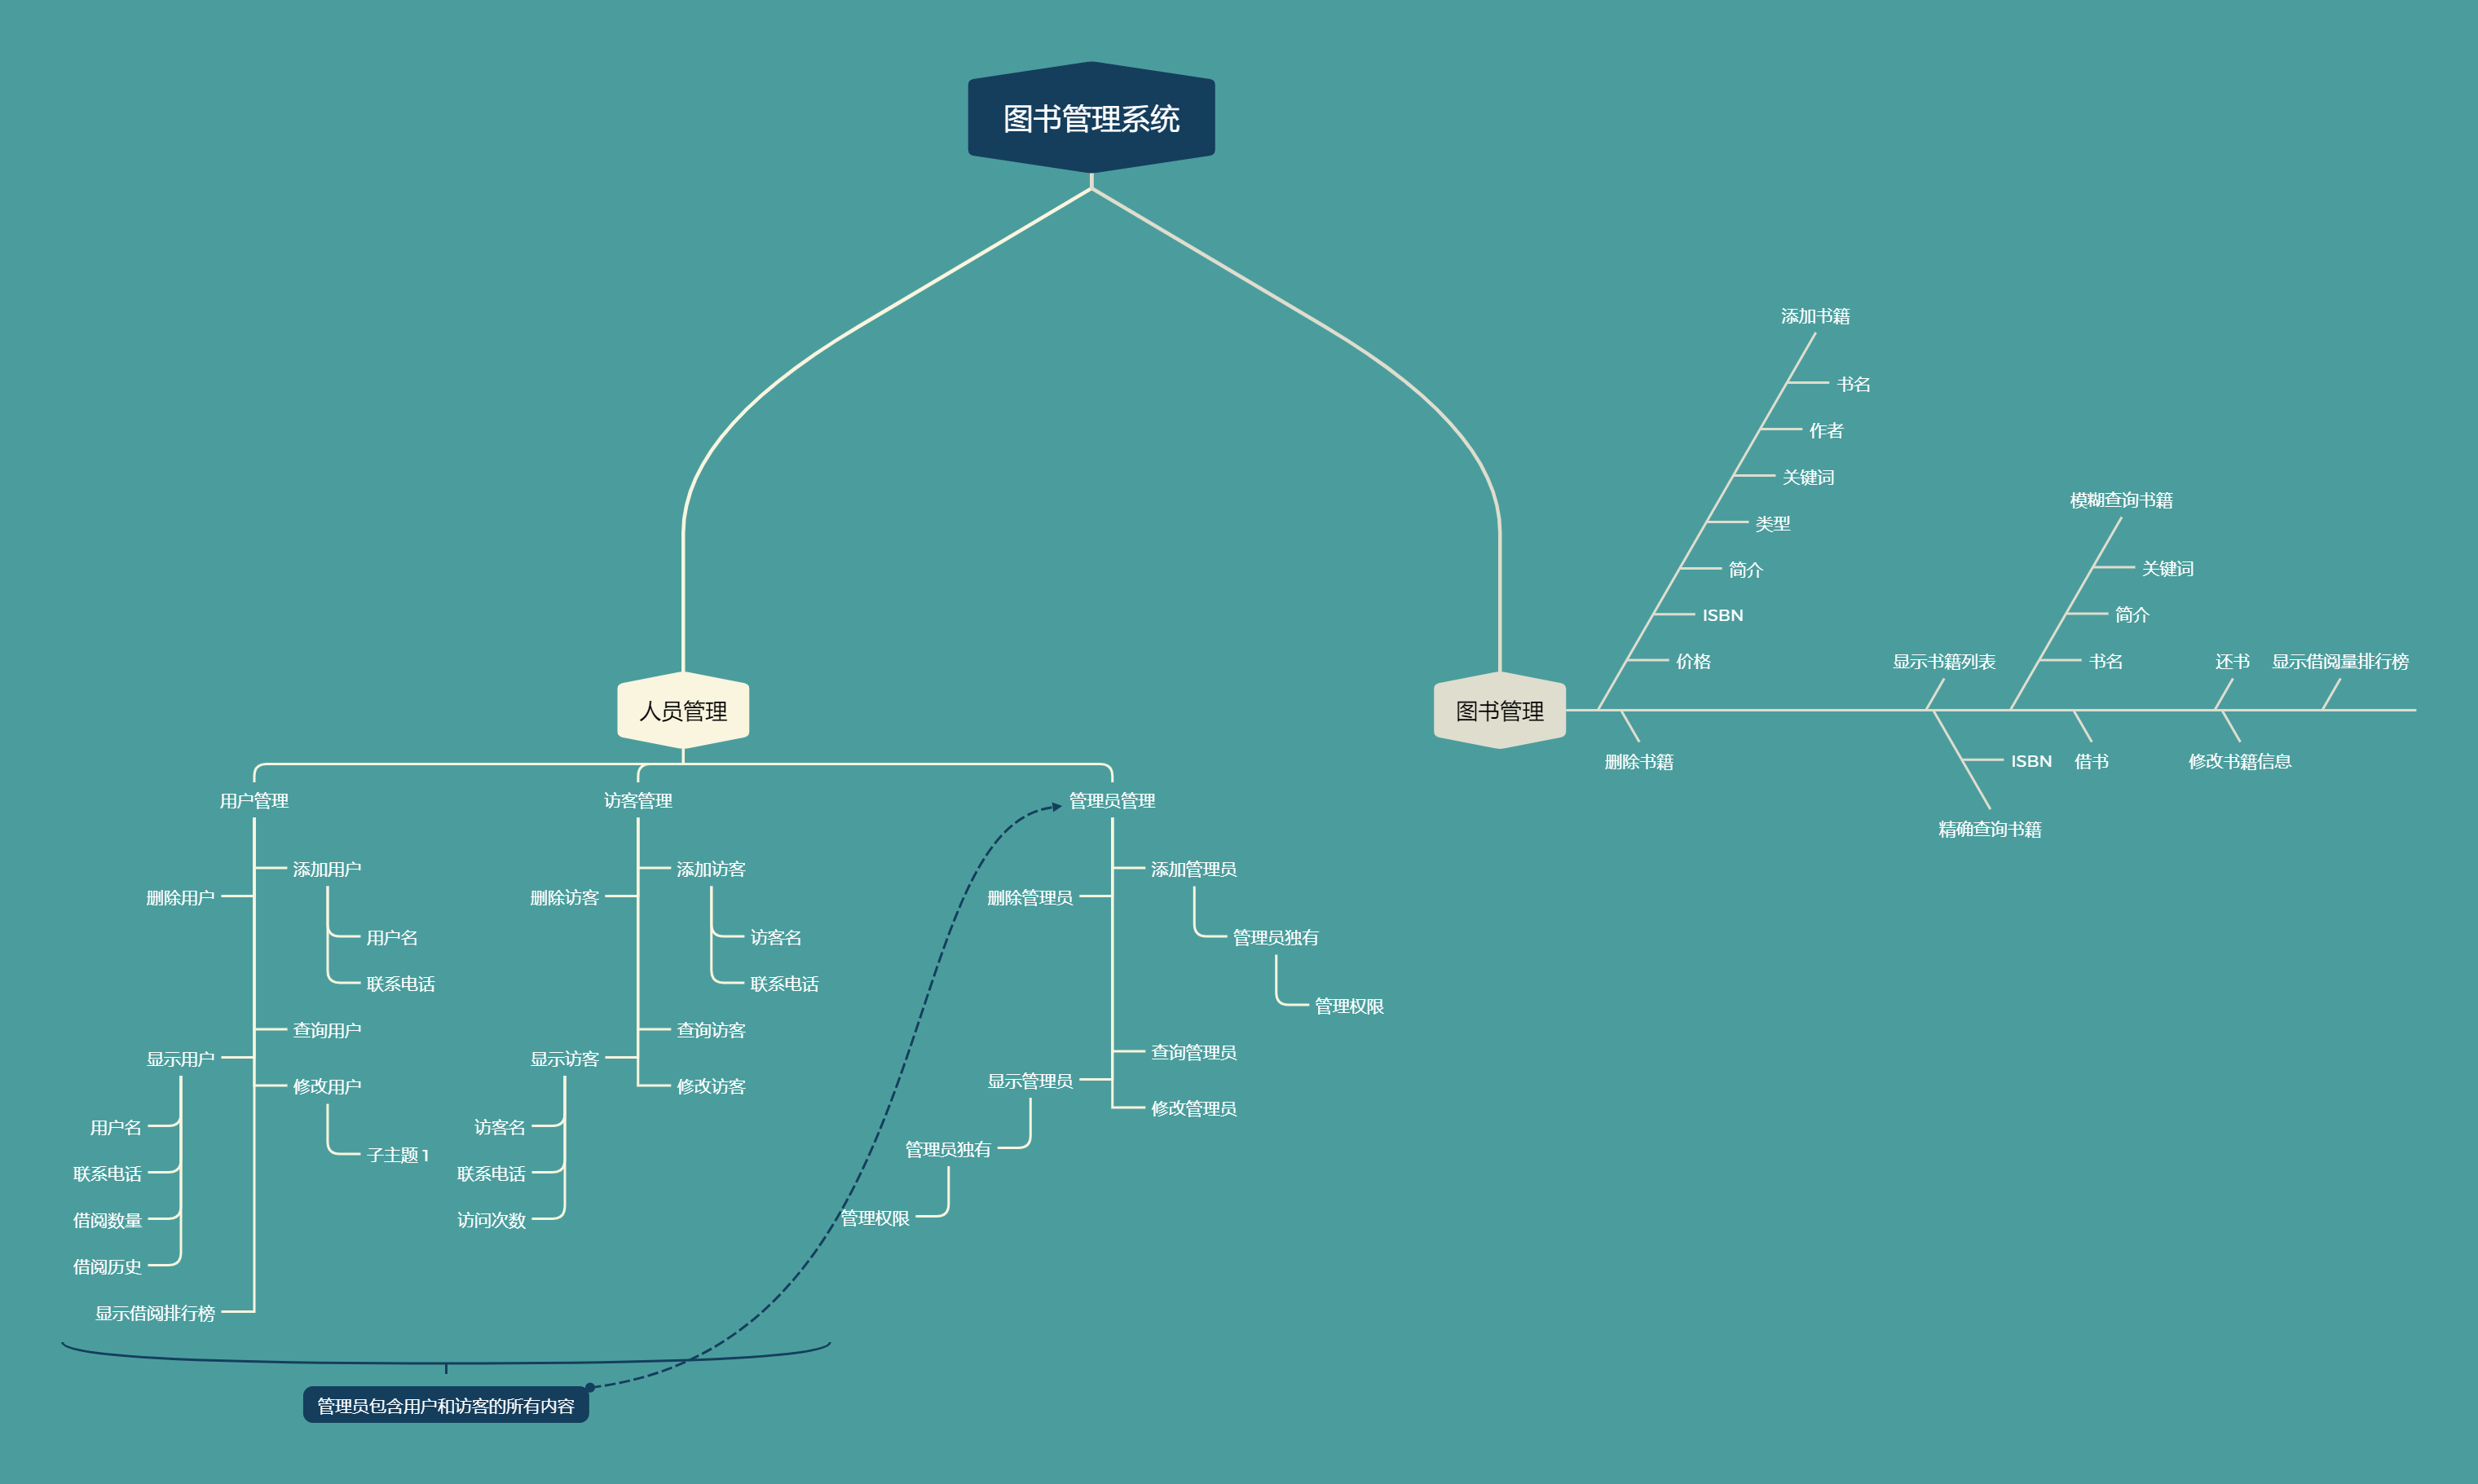
\includegraphics[width=0.6\textwidth]{total.png}
\end{figure}

\begin{figure}[H]
    \centering
    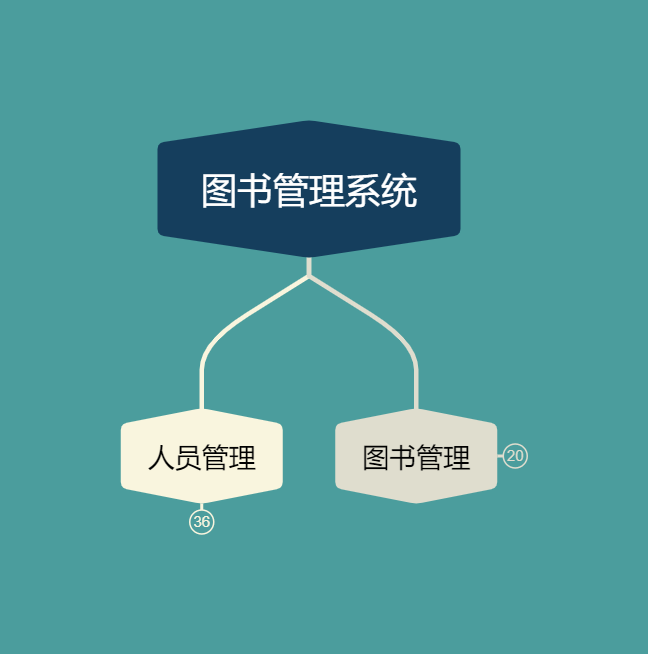
\includegraphics[width=0.5\textwidth]{part (3).png}
\end{figure}

\begin{figure}[H]
    \centering
    \begin{minipage}{0.49\textwidth}
        \centering
        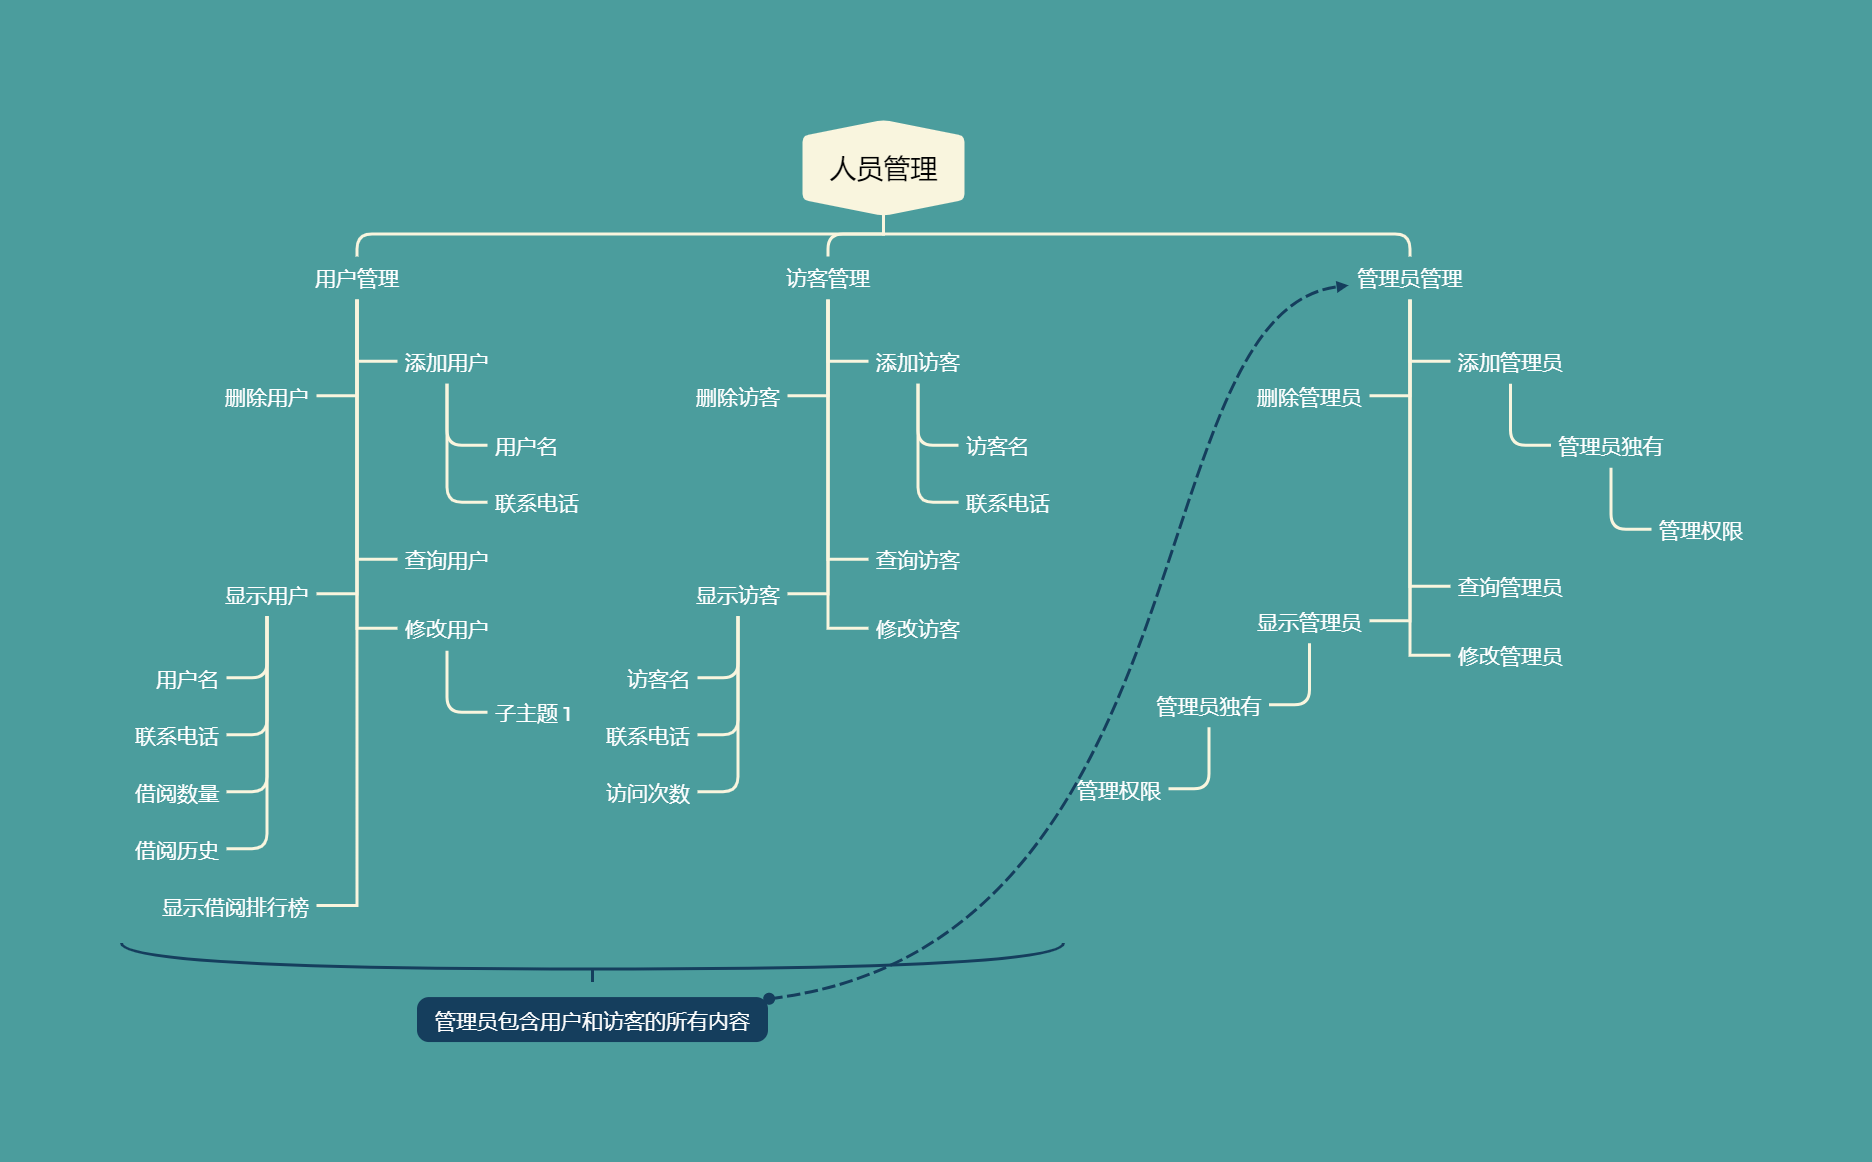
\includegraphics[width=\linewidth]{part (1).png}
    \end{minipage}
    \hfill
    \begin{minipage}{0.49\textwidth}
        \centering
        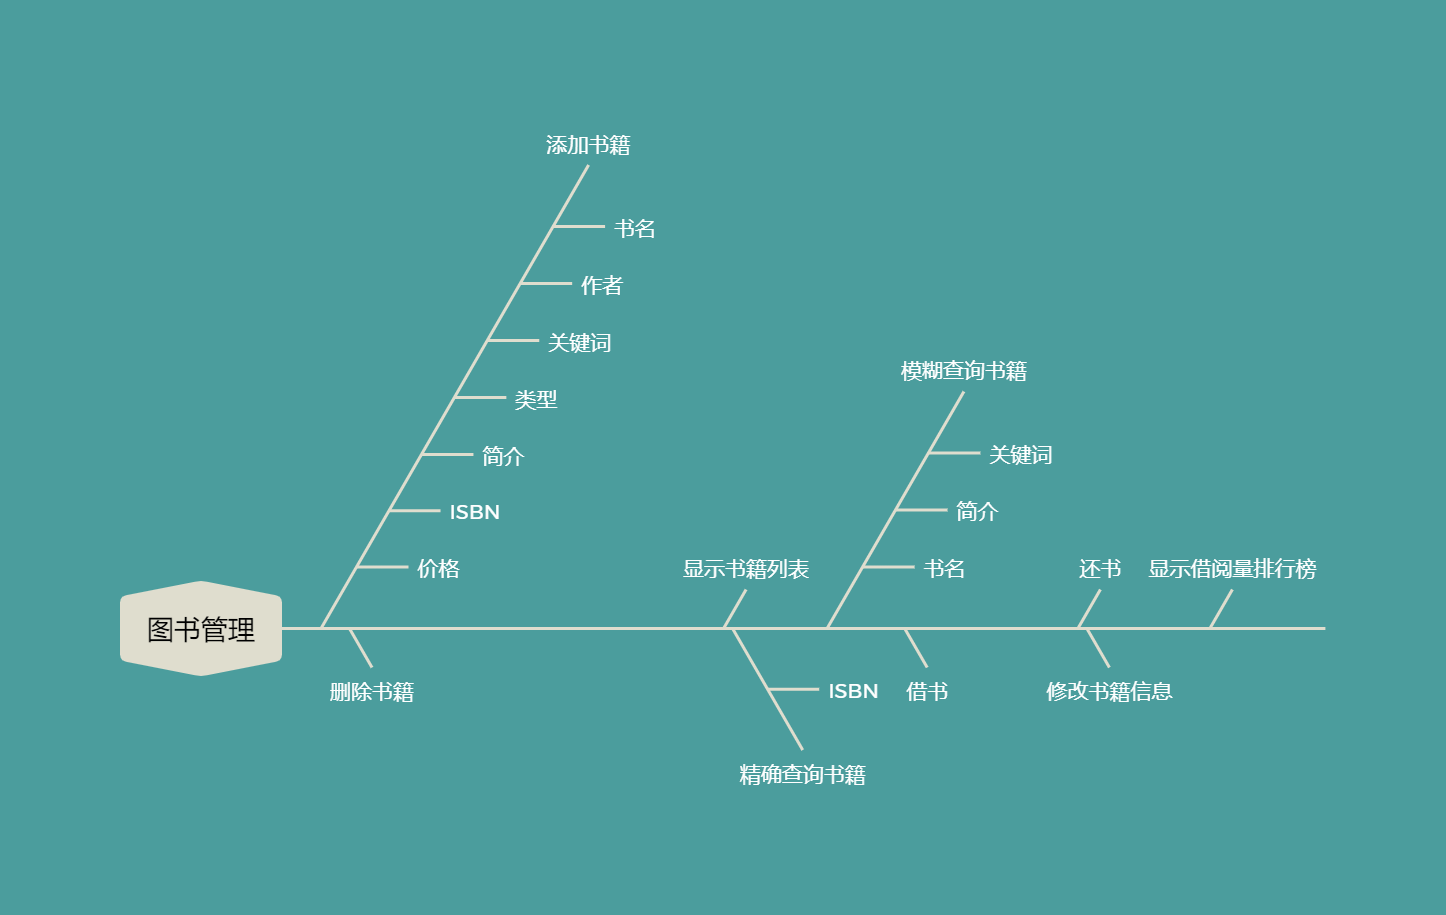
\includegraphics[width=\linewidth]{part (2).png}
    \end{minipage}
\end{figure}

\section{系统功能}

\subsection{进入系统}

\begin{figure}[H]
    \centering
    \begin{minipage}{0.48\textwidth}
        \centering
        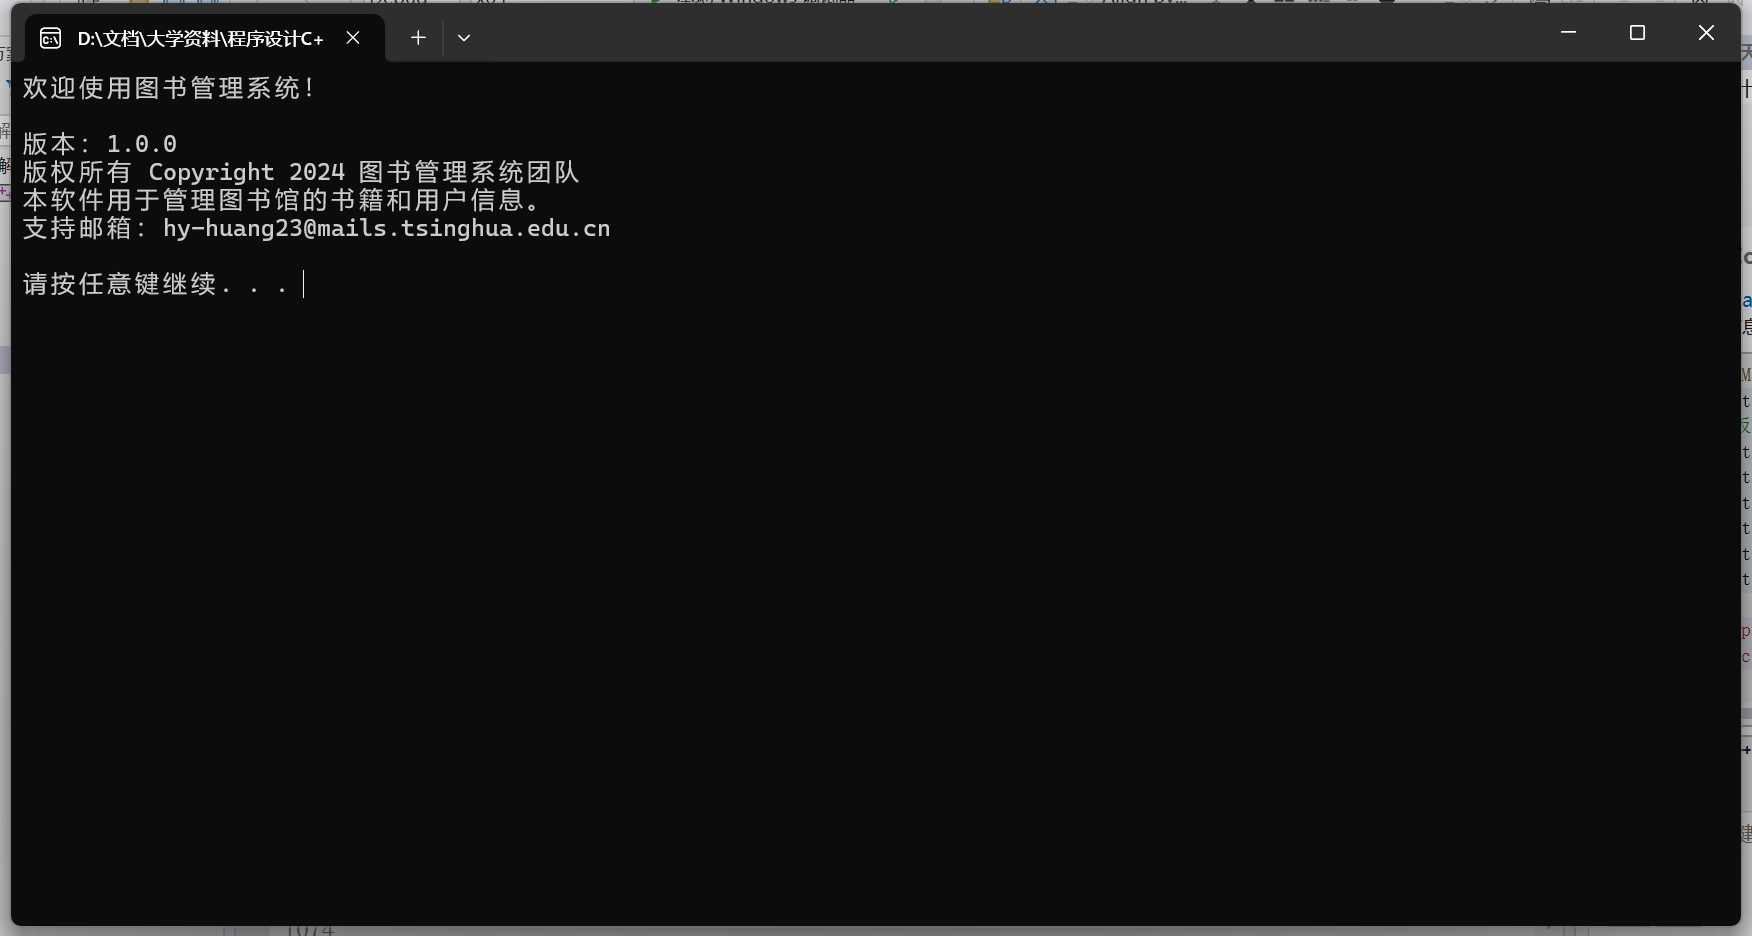
\includegraphics[width=\linewidth]{Begining.png}
        \caption{开始界面}
    \end{minipage}\hfill
    \begin{minipage}{0.48\textwidth}
        \centering
        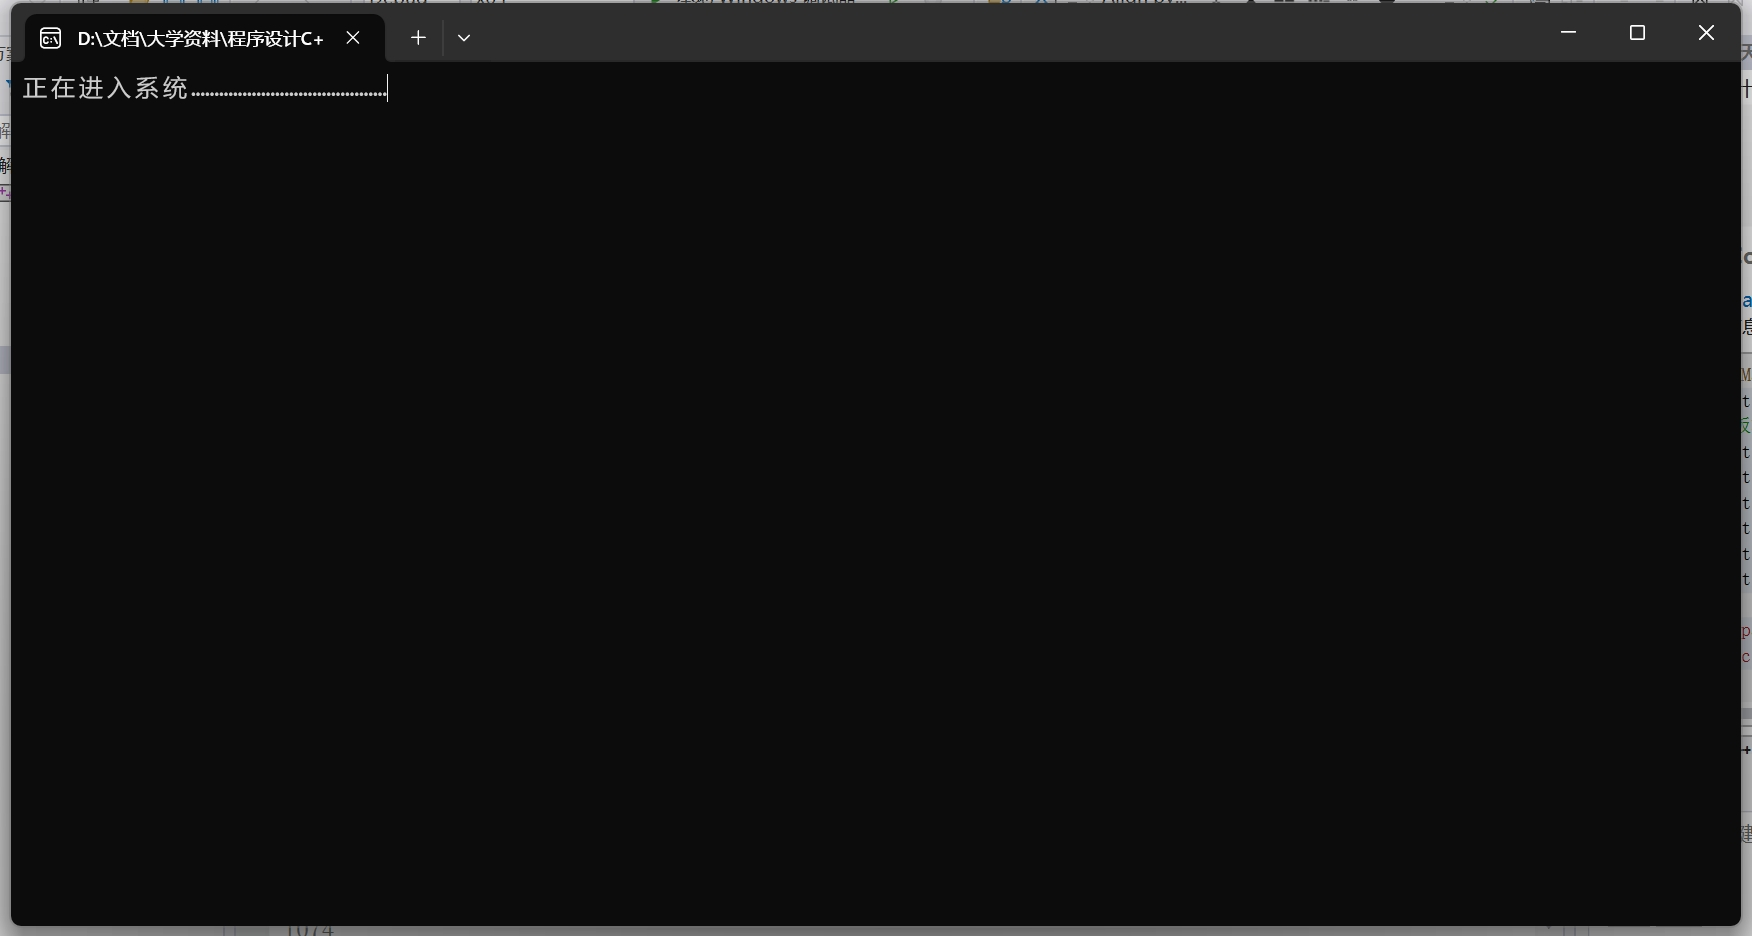
\includegraphics[width=\linewidth]{Starting.png}
        \caption{按任意键进入系统}
    \end{minipage}
\end{figure}

\begin{figure}[H]
    \centering
    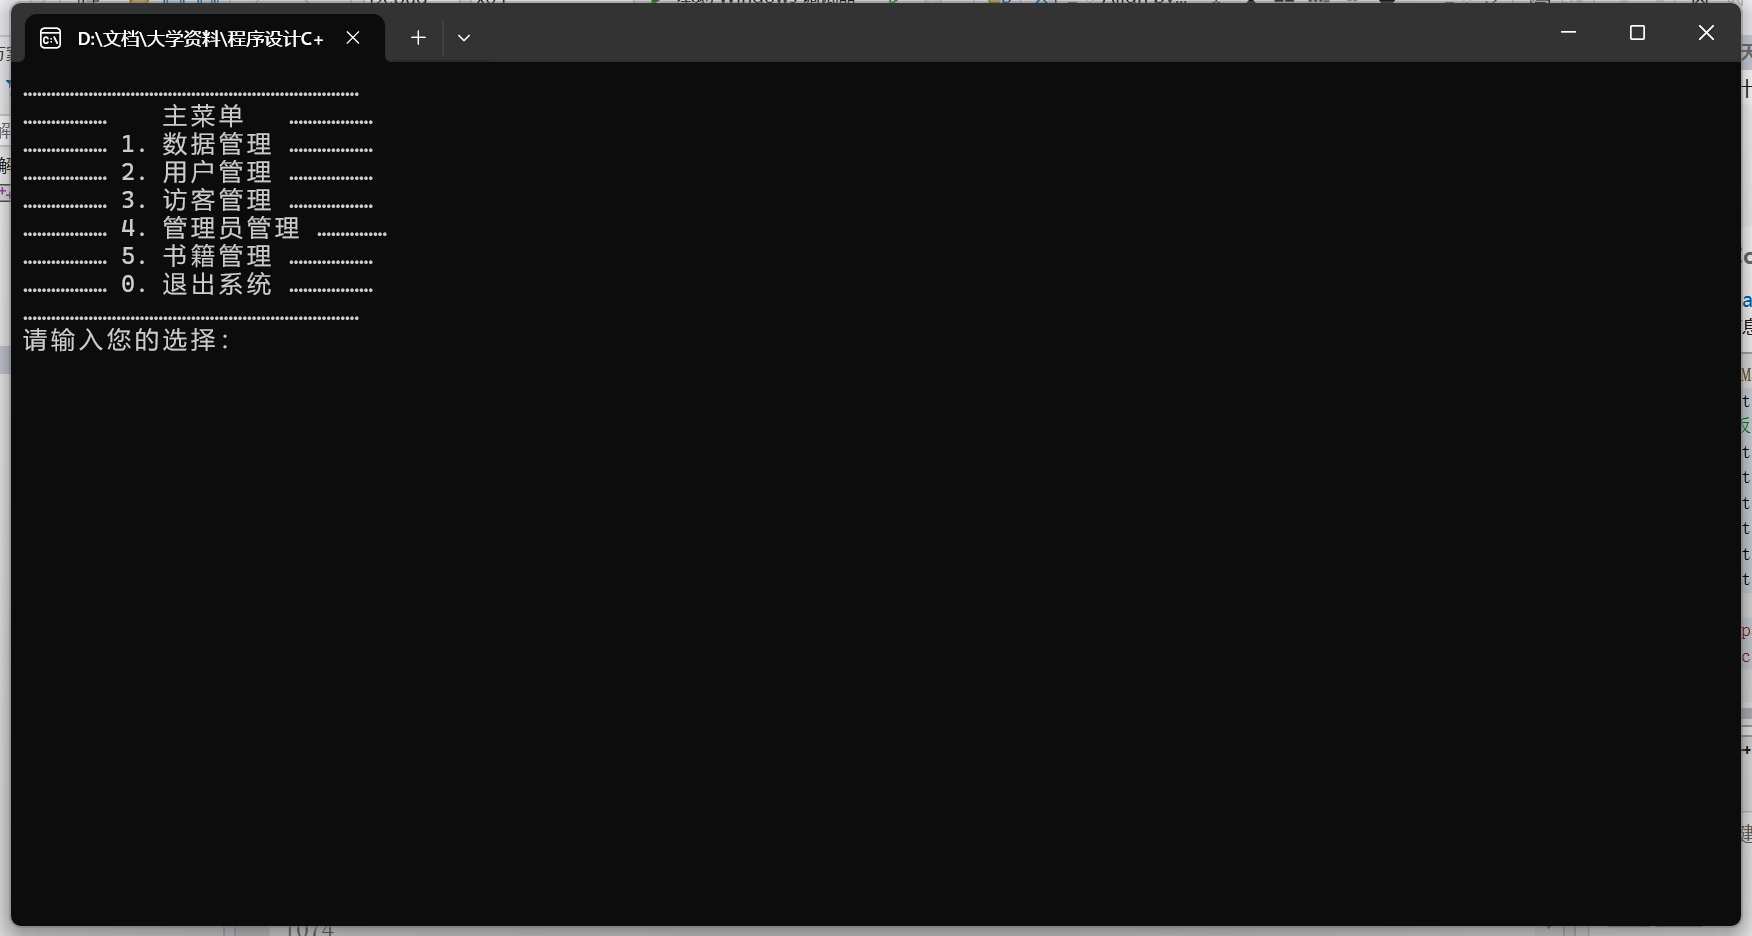
\includegraphics[width=0.8\textwidth]{Main.png}
    \caption{主菜单}
\end{figure}

\subsection{数据管理}

\begin{figure}[H]
    \centering
    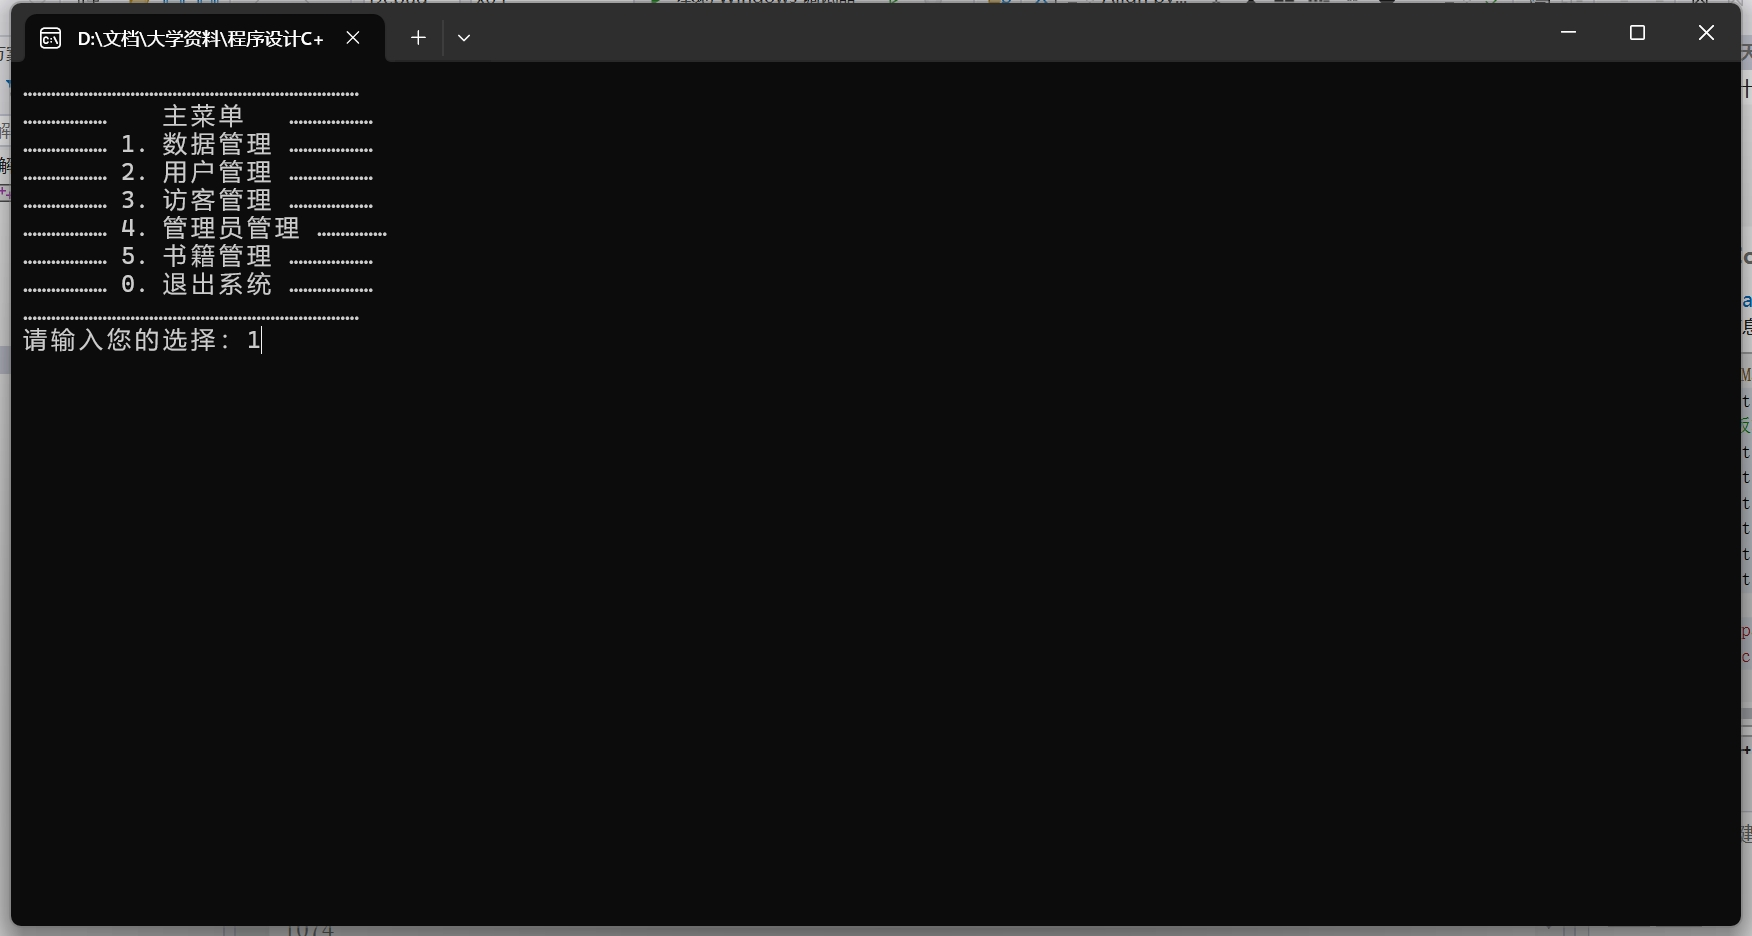
\includegraphics[width=0.8\textwidth]{SelectData.png}
    \caption{选择数据管理}
\end{figure}

\begin{figure}[H]
    \centering
    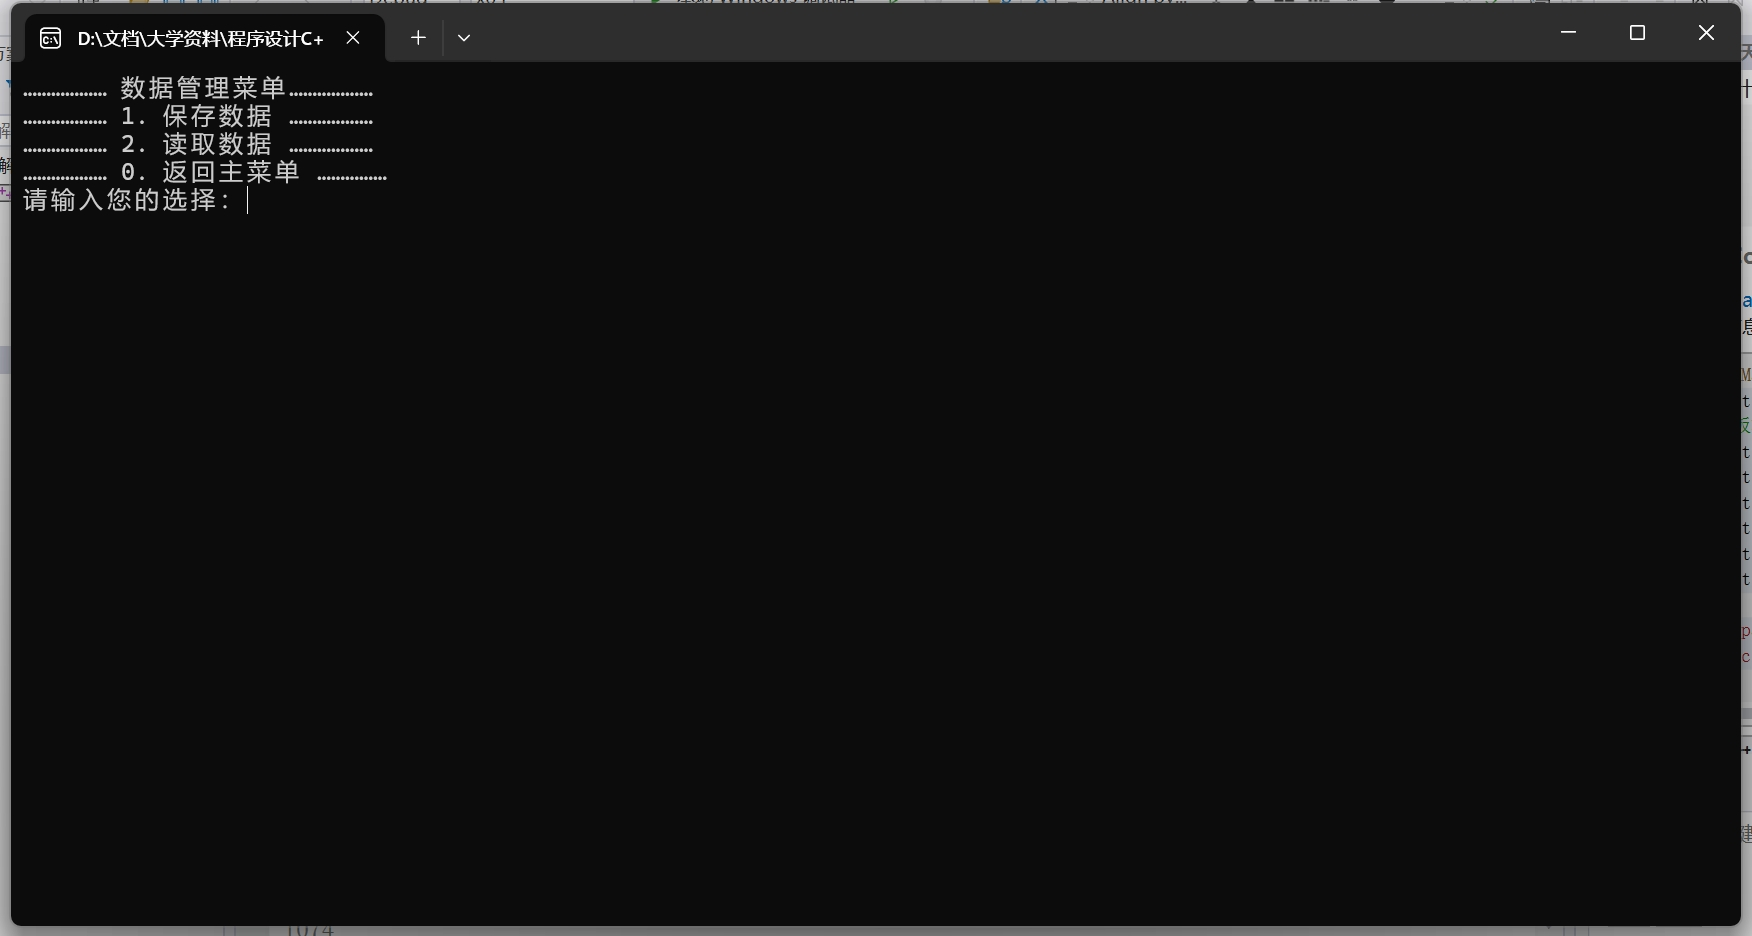
\includegraphics[width=0.8\textwidth]{DataM.png}
    \caption{进入数据管理界面}
\end{figure}

\subsubsection{读取数据}
\begin{figure}[H]
    \centering
    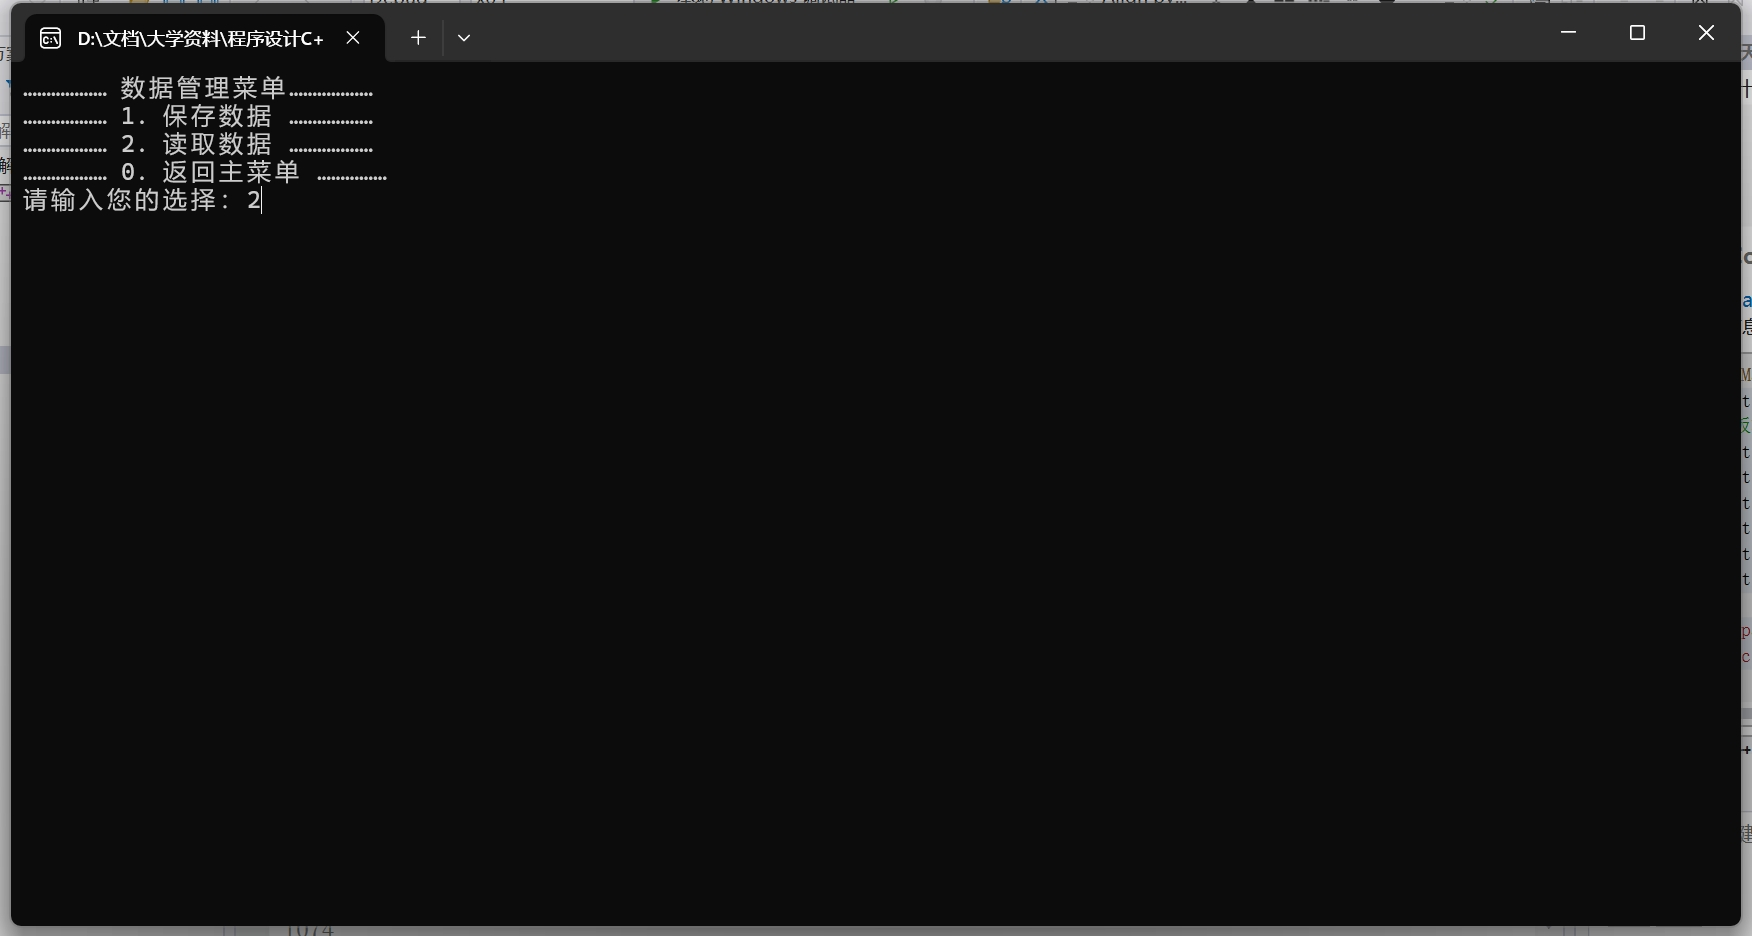
\includegraphics[width=0.8\textwidth]{ReadData.png}
    \caption{读取数据}
\end{figure}

如果读取数据成功,系统会提示读取数据成功。如图\ref{fig:ReadingData}、\ref{fig:ReadSuccessfully}所示。
\begin{figure}[H]
    \centering
    \begin{minipage}{0.48\textwidth}
        \centering
        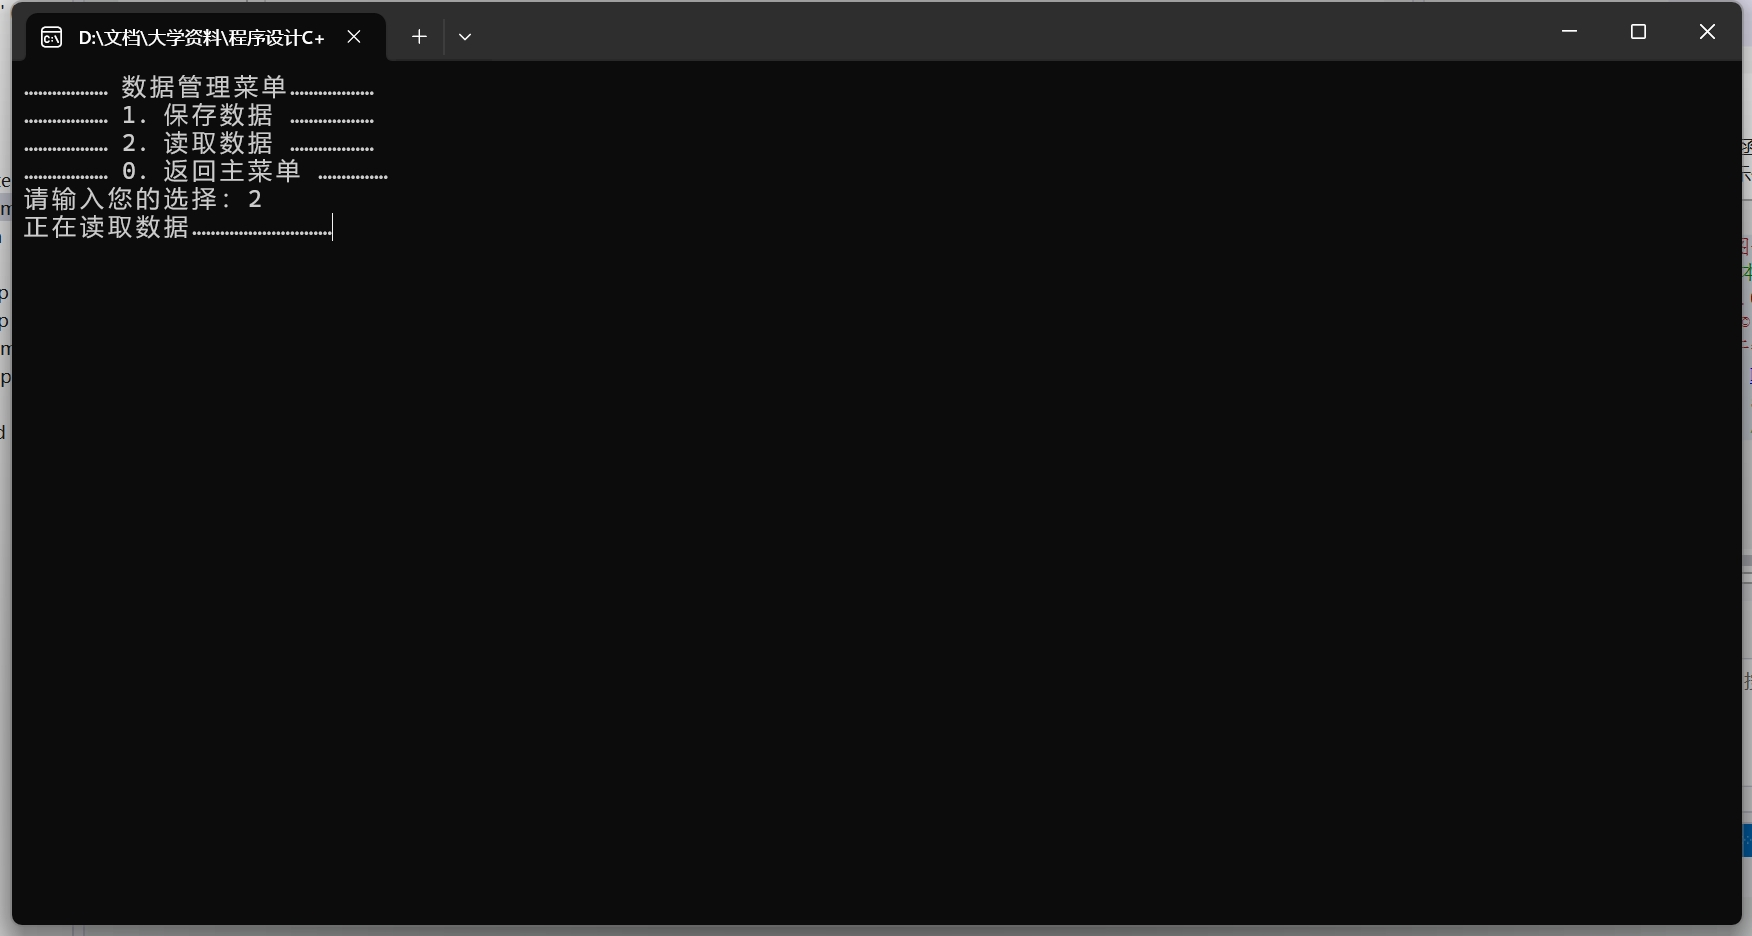
\includegraphics[width=\linewidth]{ReadingData.png}
        \caption{正在读取数据}
        \label{fig:ReadingData}
    \end{minipage}\hfill
    \begin{minipage}{0.48\textwidth}
        \centering
        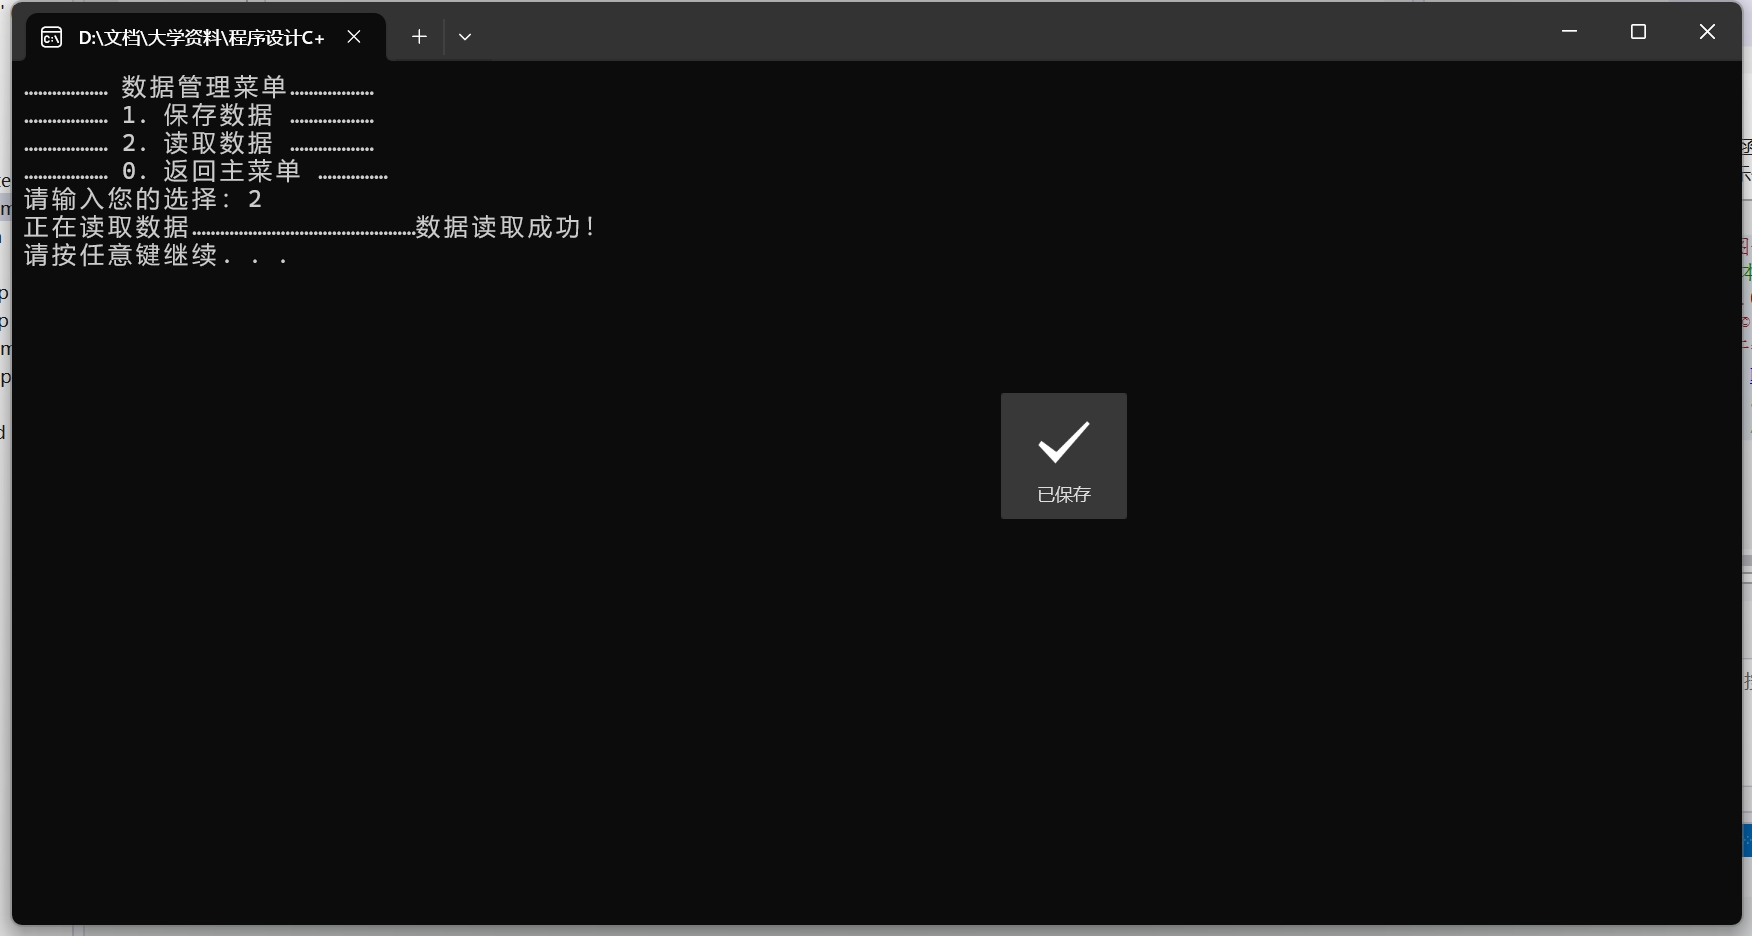
\includegraphics[width=\linewidth]{ReadSuccessfully.png}
        \caption{读取数据成功}
        \label{fig:ReadSuccessfully}
    \end{minipage}
\end{figure}

\begin{figure}[H]
    \begin{minipage}[c]{0.5\textwidth}
        $\star$ 如果读取数据失败,系统会提示读取数据失败。如图\ref{fig:ReadFailed}所示。出现这种情况可能是因为数据文件不存在或者数据文件损坏,用户可以检查数据文件是否存在或者尝试重新读取数据。
    \end{minipage}%
    \hfill
    \begin{minipage}[c]{0.45\textwidth}
        \centering
        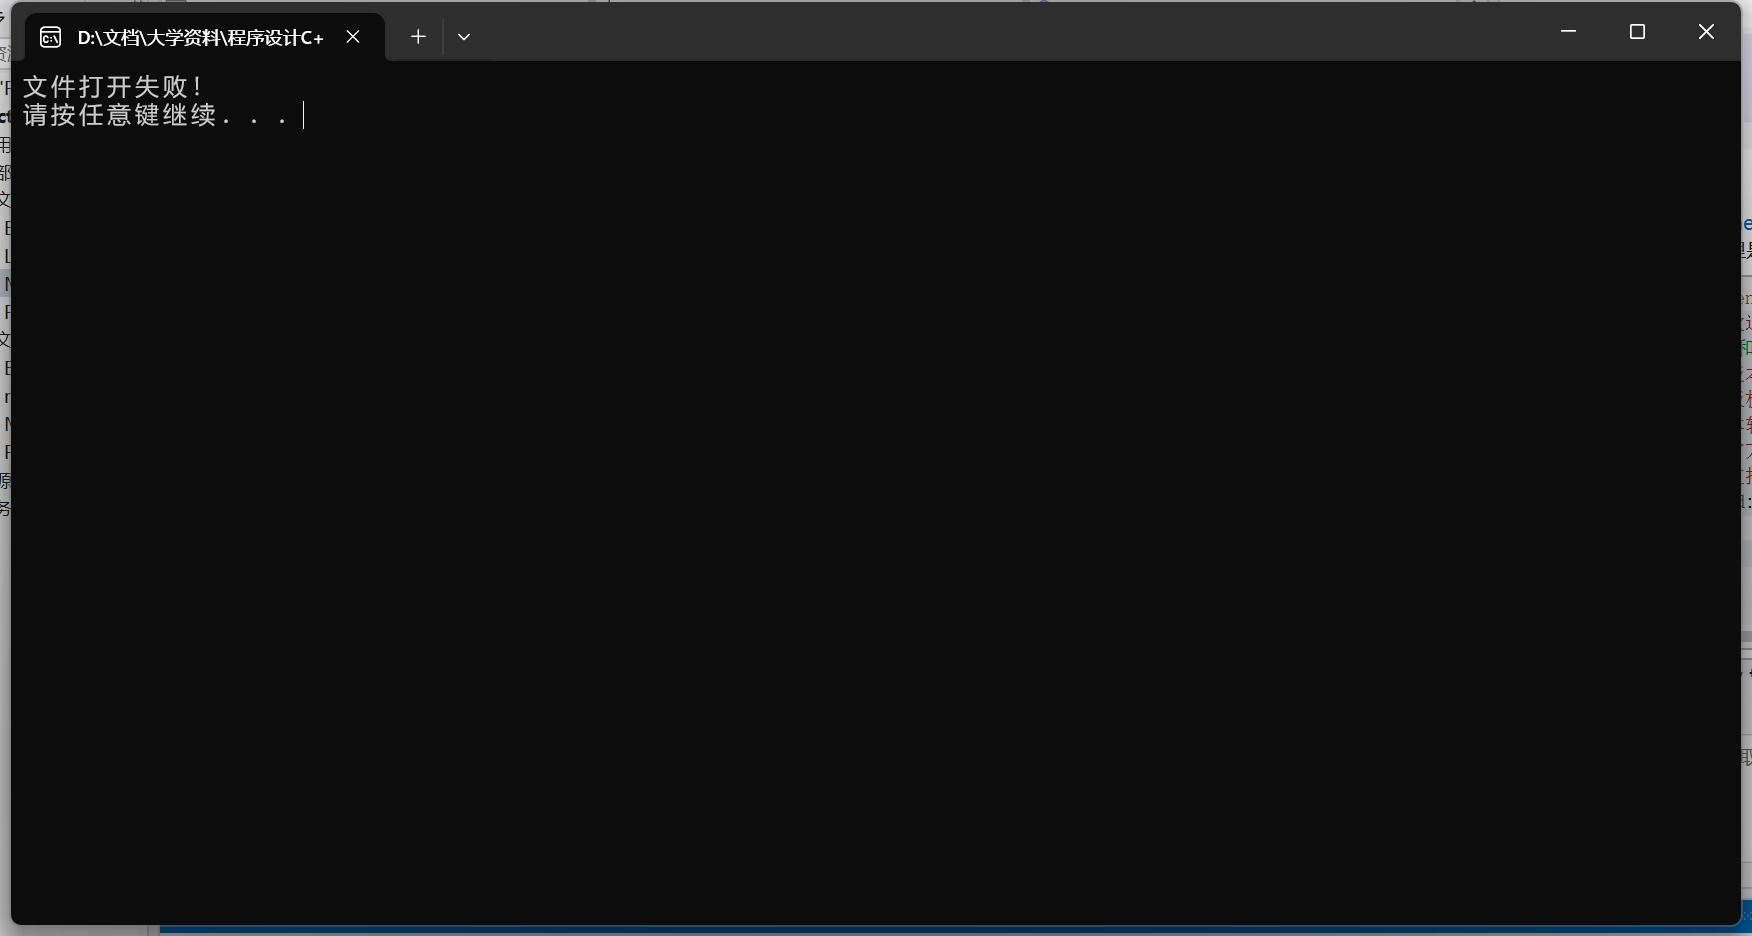
\includegraphics[width=\textwidth]{ReadFailed.png}
        \caption{读取数据失败}
        \label{fig:ReadFailed}
    \end{minipage}
\end{figure}

\begin{figure}[H]
    \centering
    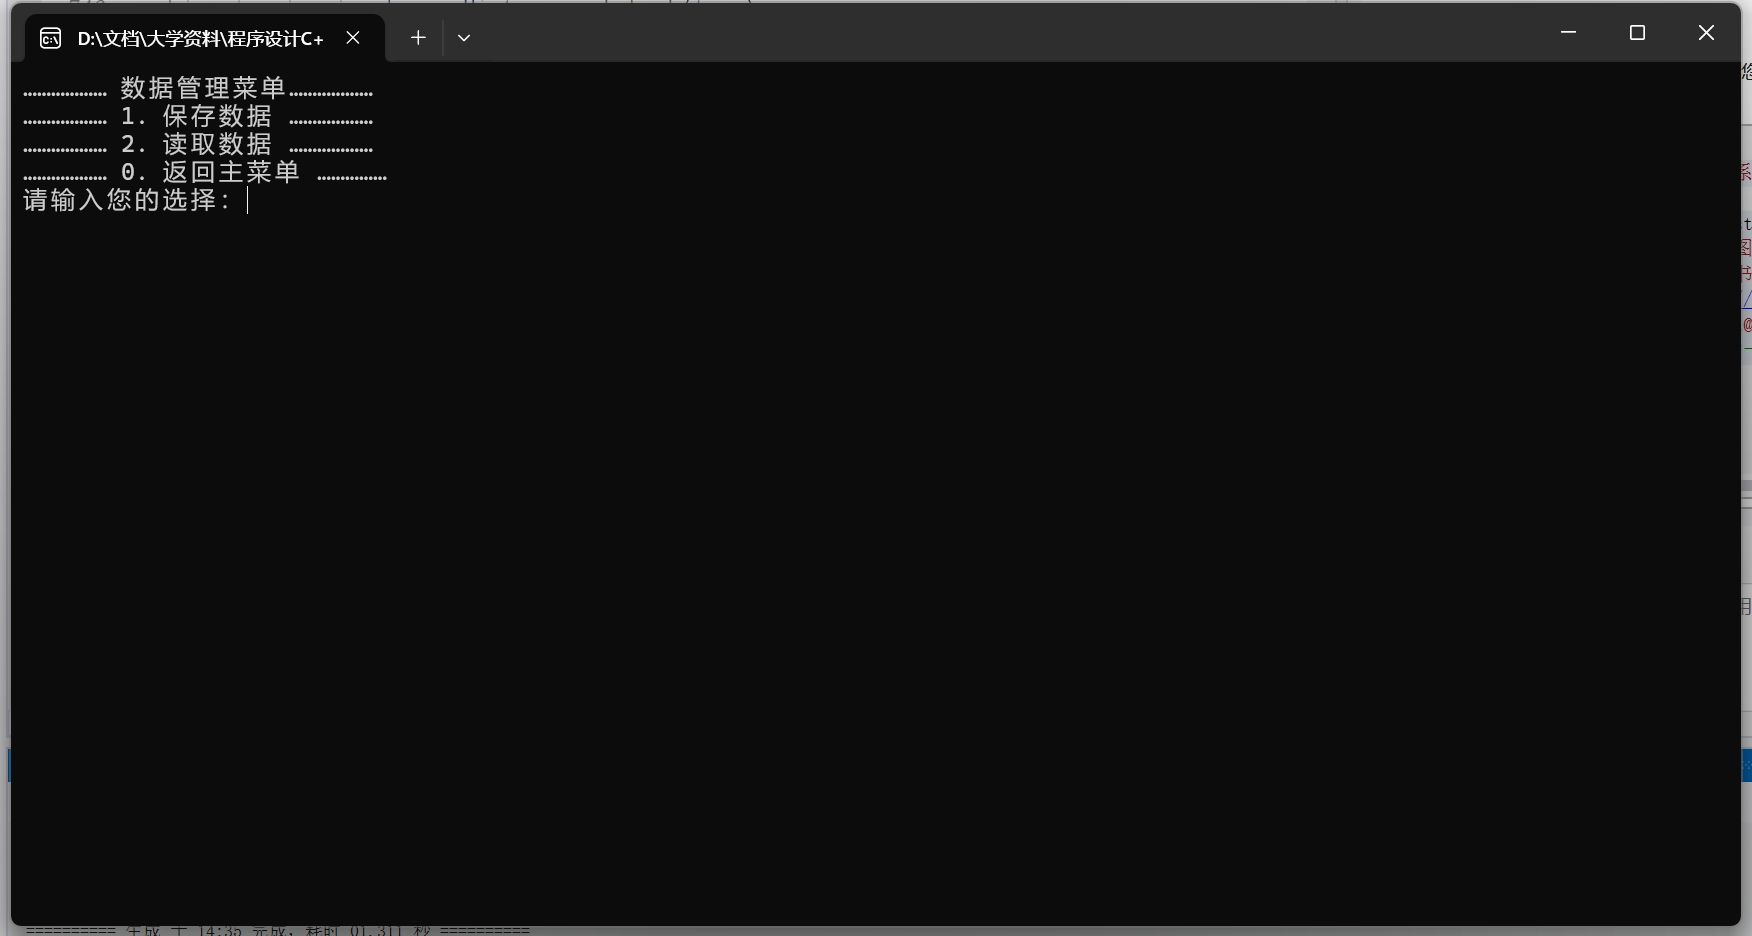
\includegraphics[width=0.8\textwidth]{ReadReturn.png}
    \caption{返回数据管理界面}
\end{figure}

\subsubsection{保存数据}
\begin{figure}[H]
    \centering
    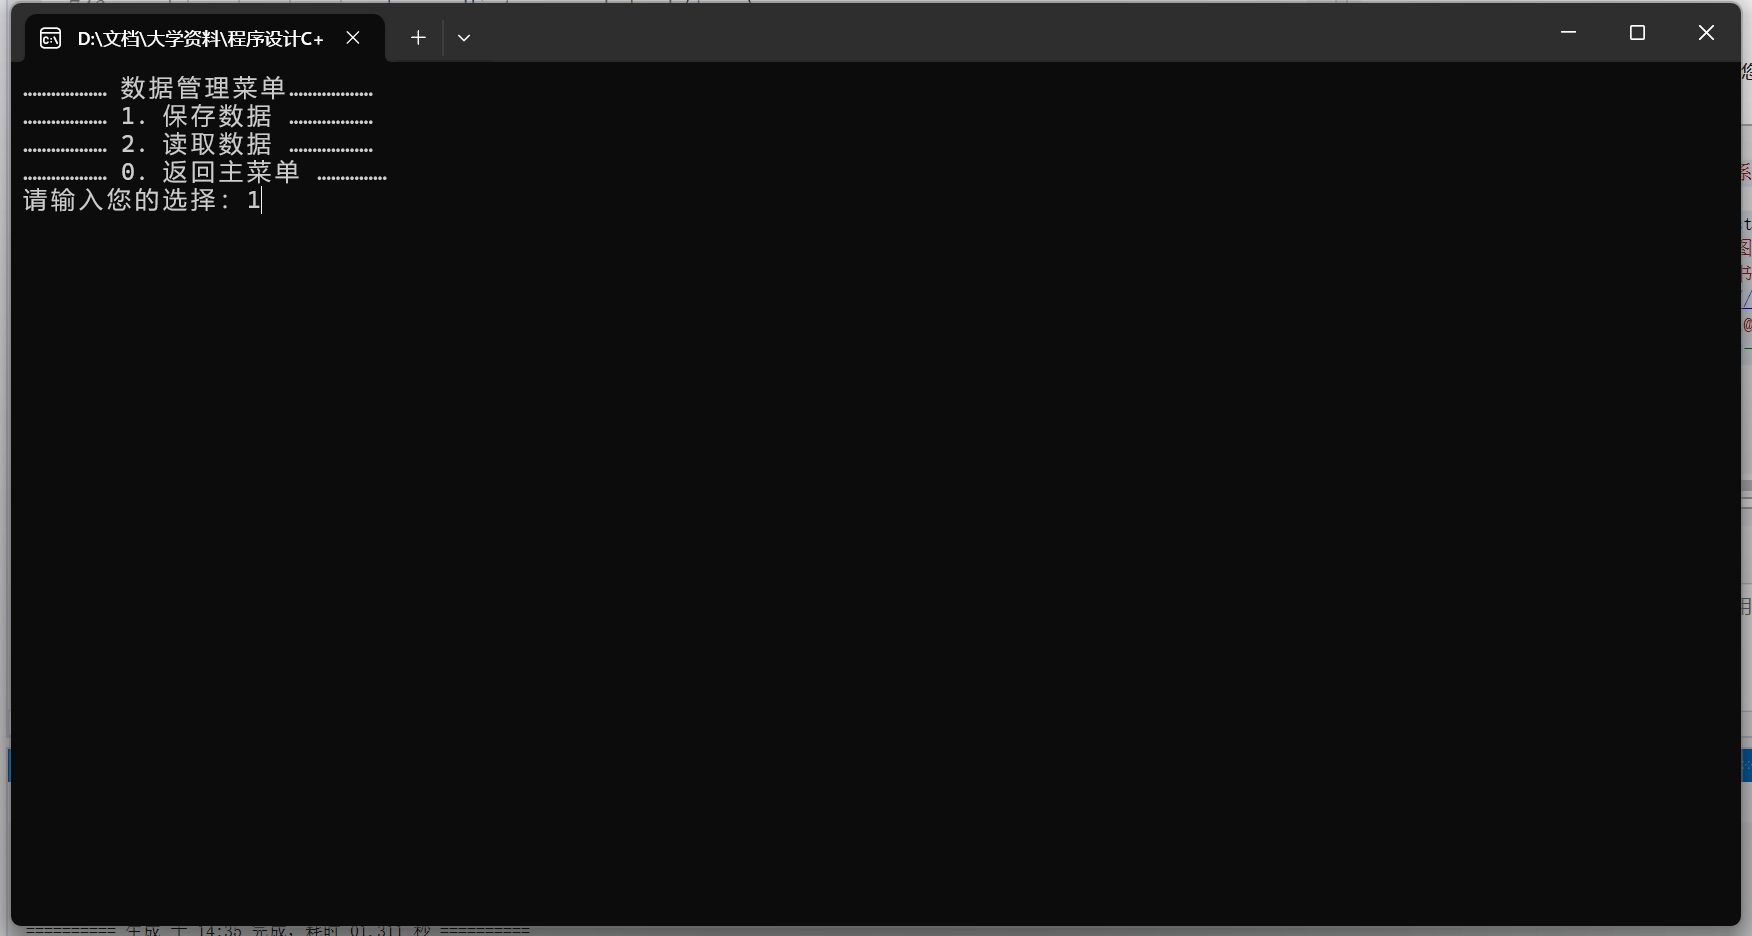
\includegraphics[width=0.8\textwidth]{SaveData.png}
    \caption{保存数据}
\end{figure}

如果保存数据成功,系统会提示保存数据成功。如图\ref{fig:SavingData}、\ref{fig:SaveSuccessfully}所示。
\begin{figure}[H]
    \centering
    \begin{minipage}{0.48\textwidth}
        \centering
        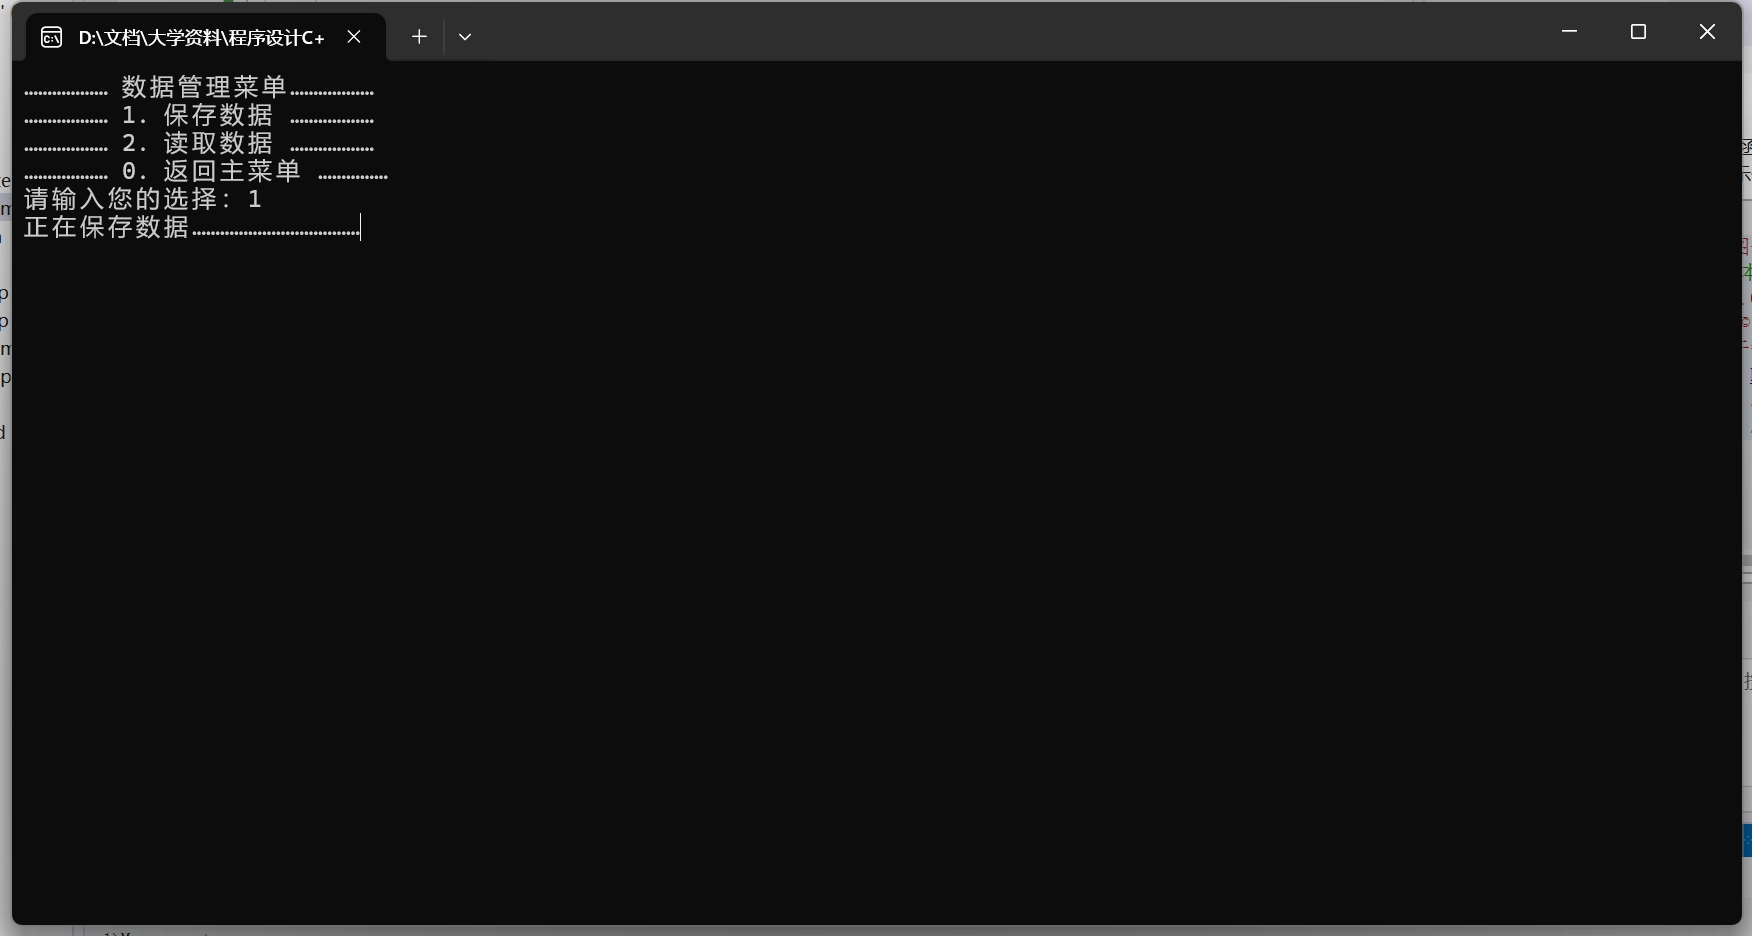
\includegraphics[width=\linewidth]{SavingData.png}
        \caption{正在保存数据}
        \label{fig:SavingData}
    \end{minipage}\hfill
    \begin{minipage}{0.48\textwidth}
        \centering
        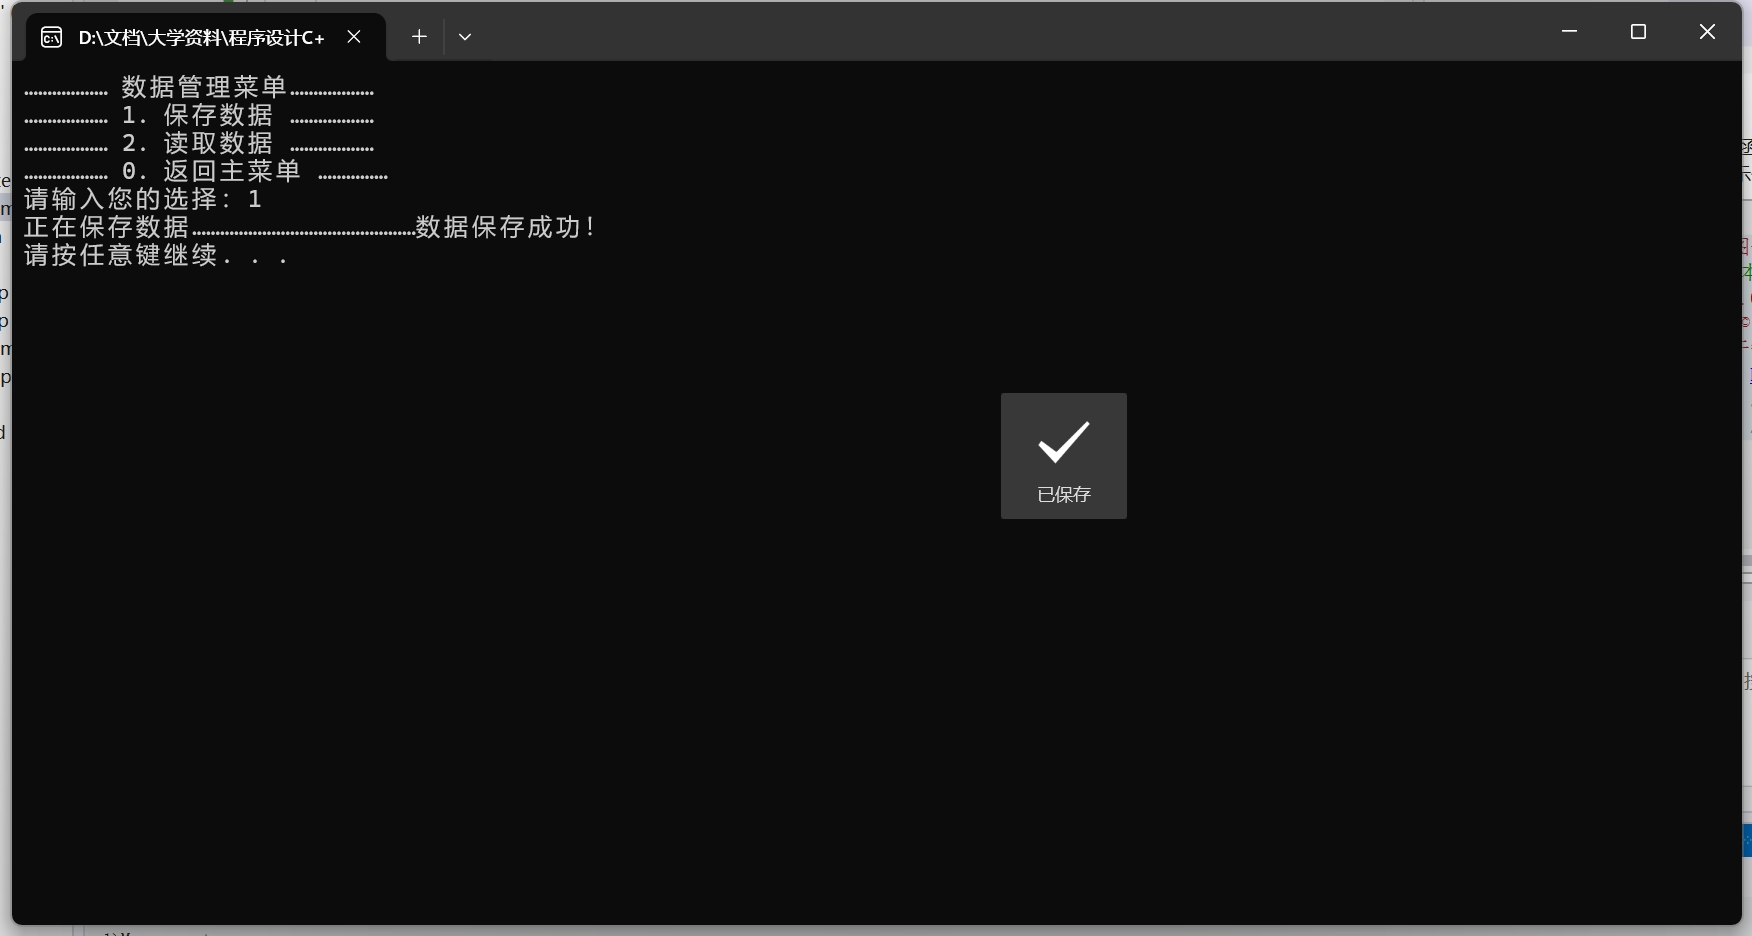
\includegraphics[width=\linewidth]{SaveDataSuccfully.png}
        \caption{保存数据成功}
        \label{fig:SaveSuccessfully}
    \end{minipage}
\end{figure}

\begin{figure}[H]
    \begin{minipage}[c]{0.5\textwidth}
        $\star$ 保存数据一般不会出现失败的情况,如果保存失败,可能是因为磁盘空间不足或者磁盘损坏等原因,
        用户可以检查磁盘空间是否足够或者尝试重新保存数据,如图\ref{fig:CheckAvailable}所示。
    \end{minipage}%
    \hfill
    \begin{minipage}[c]{0.45\textwidth}
        \centering
        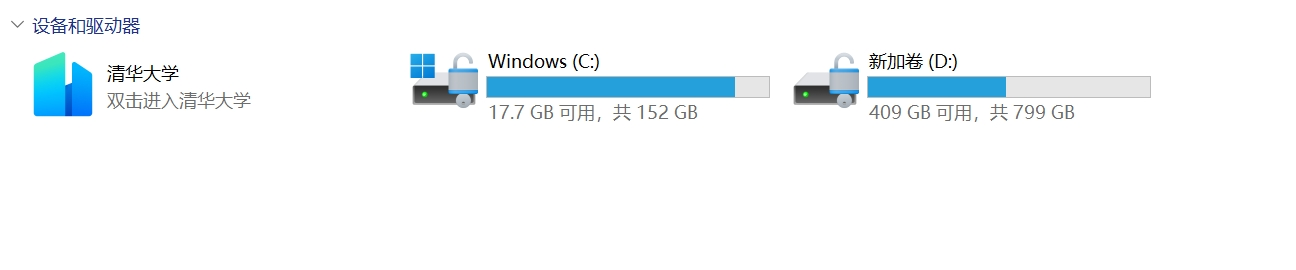
\includegraphics[width=\textwidth]{CheckAvailable.png}
        \caption{检查磁盘空间}
        \label{fig:CheckAvailable}
    \end{minipage}
\end{figure}

\begin{figure}[H]
    \centering
    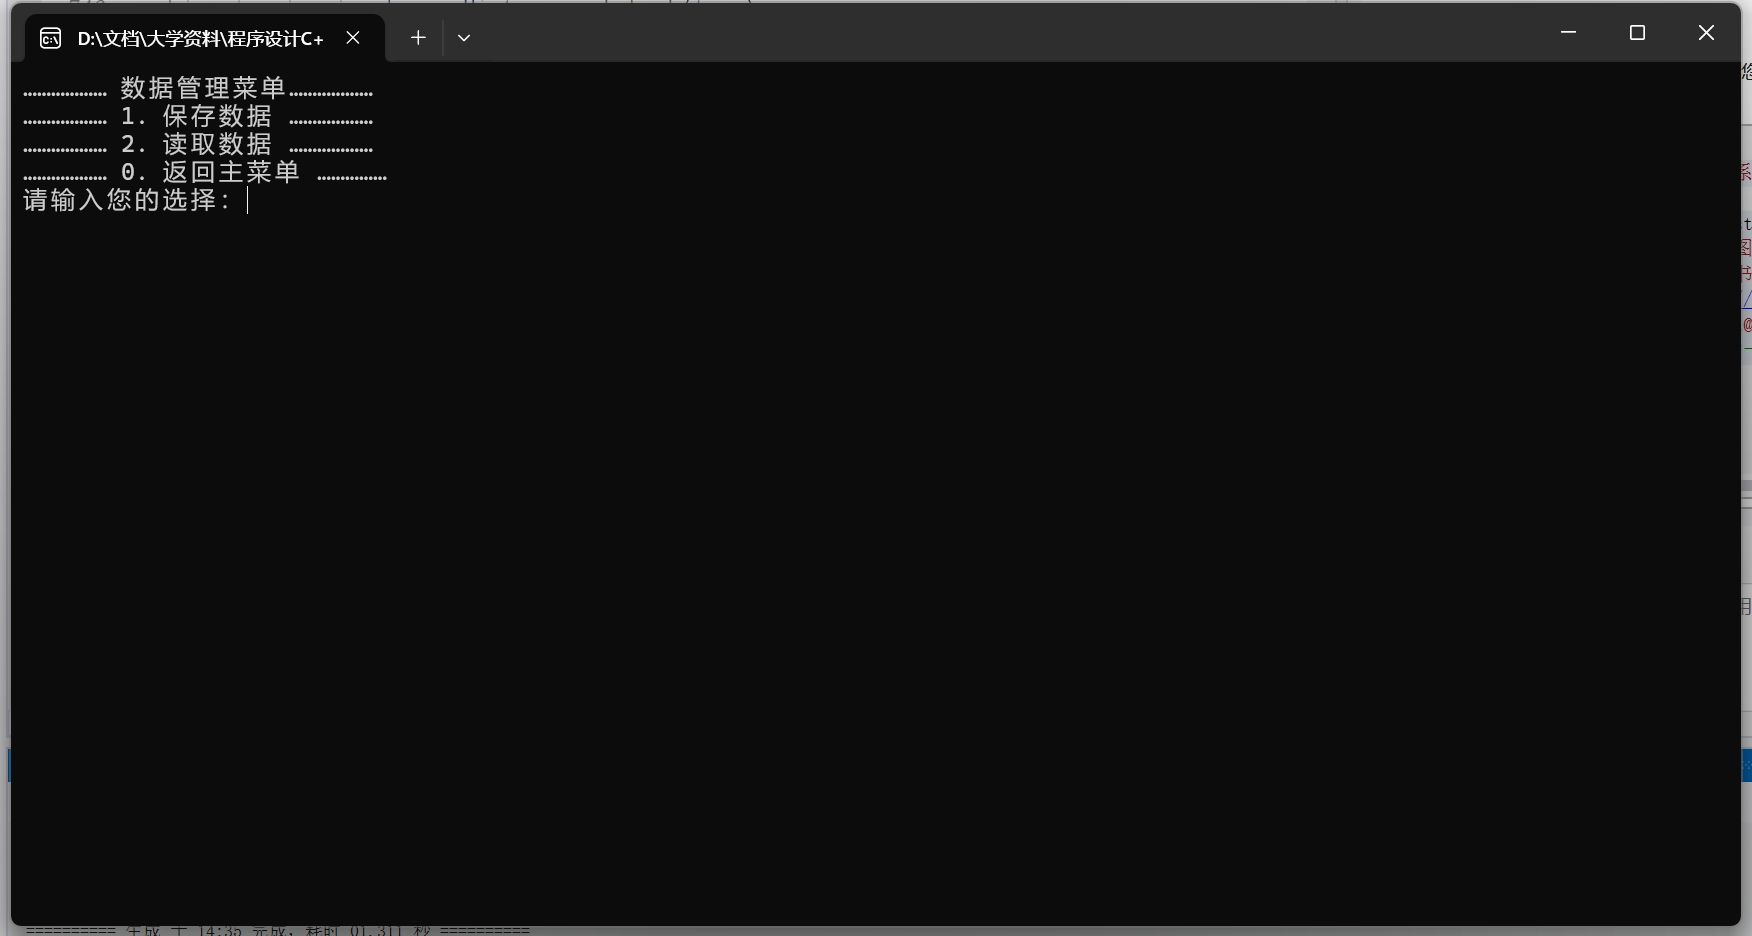
\includegraphics[width=0.8\textwidth]{ReadReturn.png}
    \caption{返回数据管理界面}
\end{figure}

\newpage
\subsection{用户管理}

\begin{figure}[H]
    \centering
    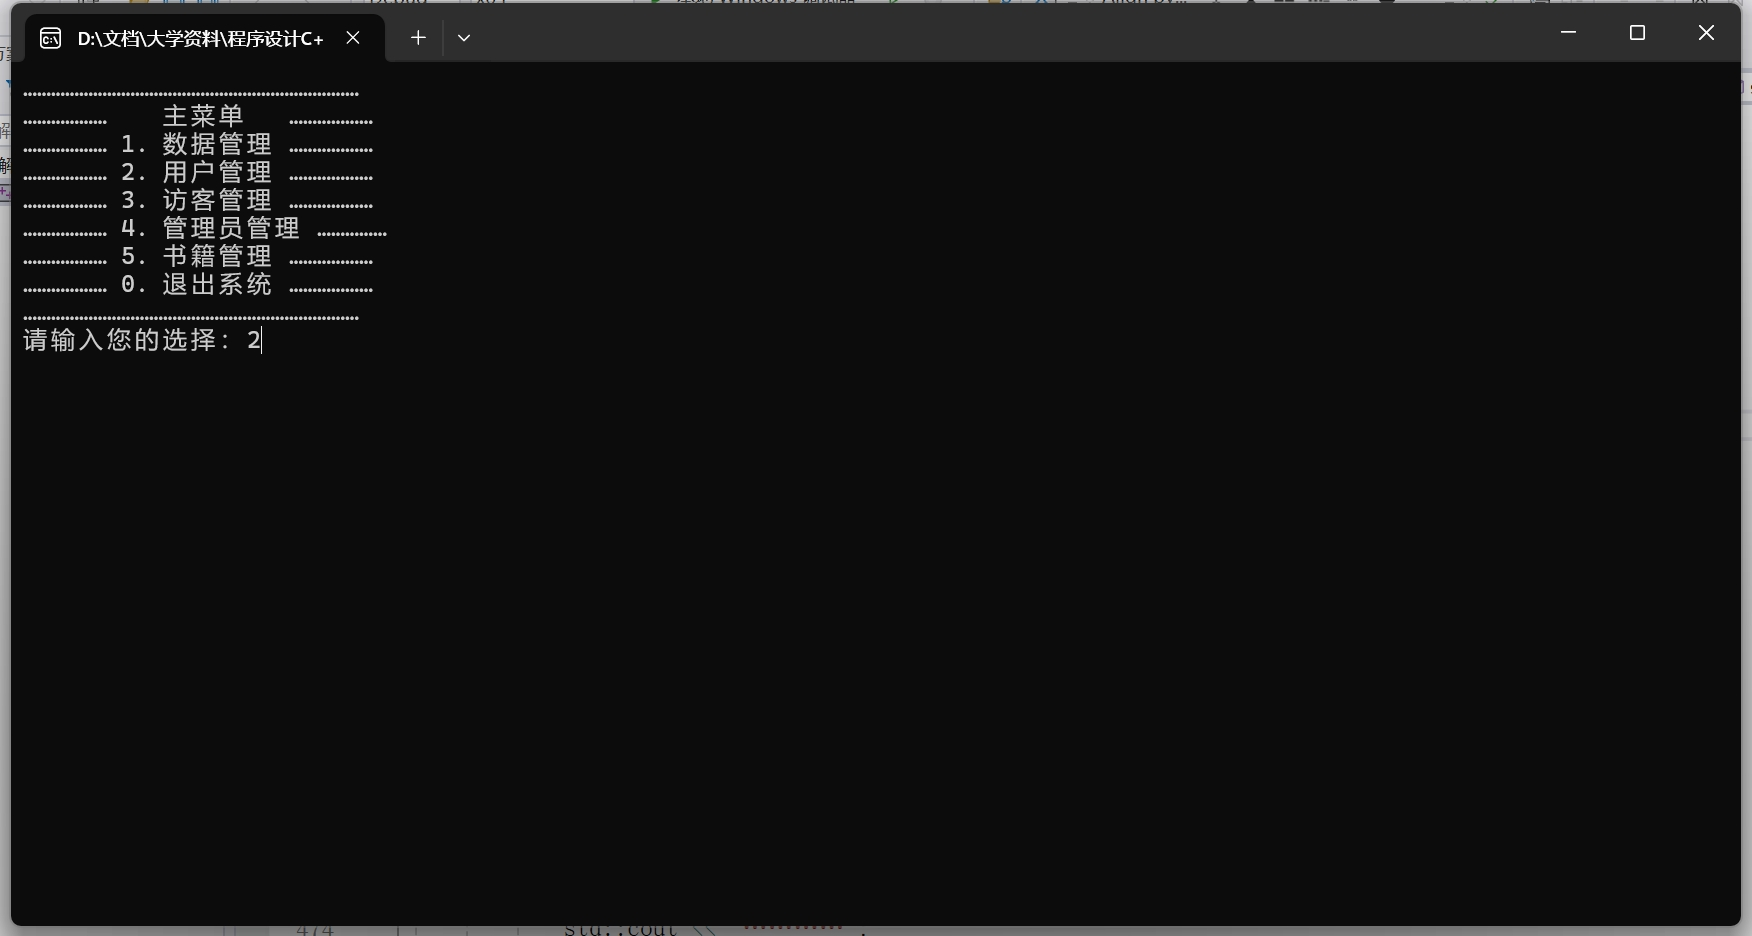
\includegraphics[width=0.8\textwidth]{SelectUser.png}
    \caption{选择用户管理}
\end{figure}

\begin{figure}[H]
    \centering
    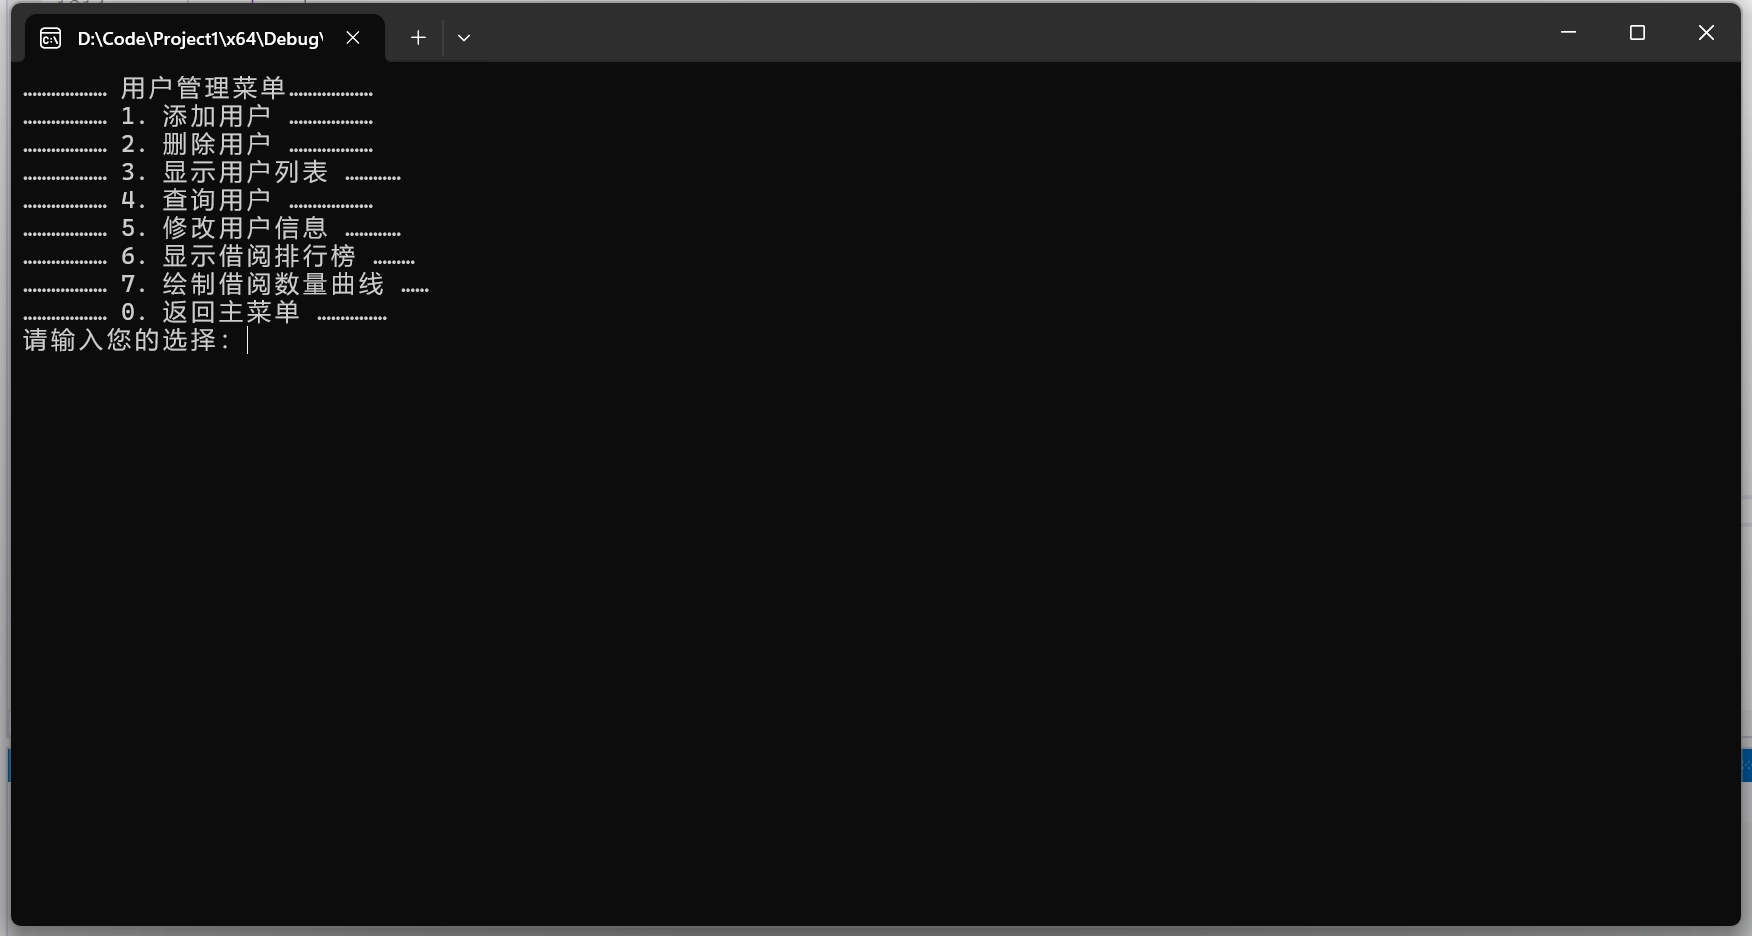
\includegraphics[width=0.8\textwidth]{User.png}
    \caption{进入用户管理界面}
\end{figure}

\subsubsection{添加用户}
\begin{figure}[H]
    \centering
    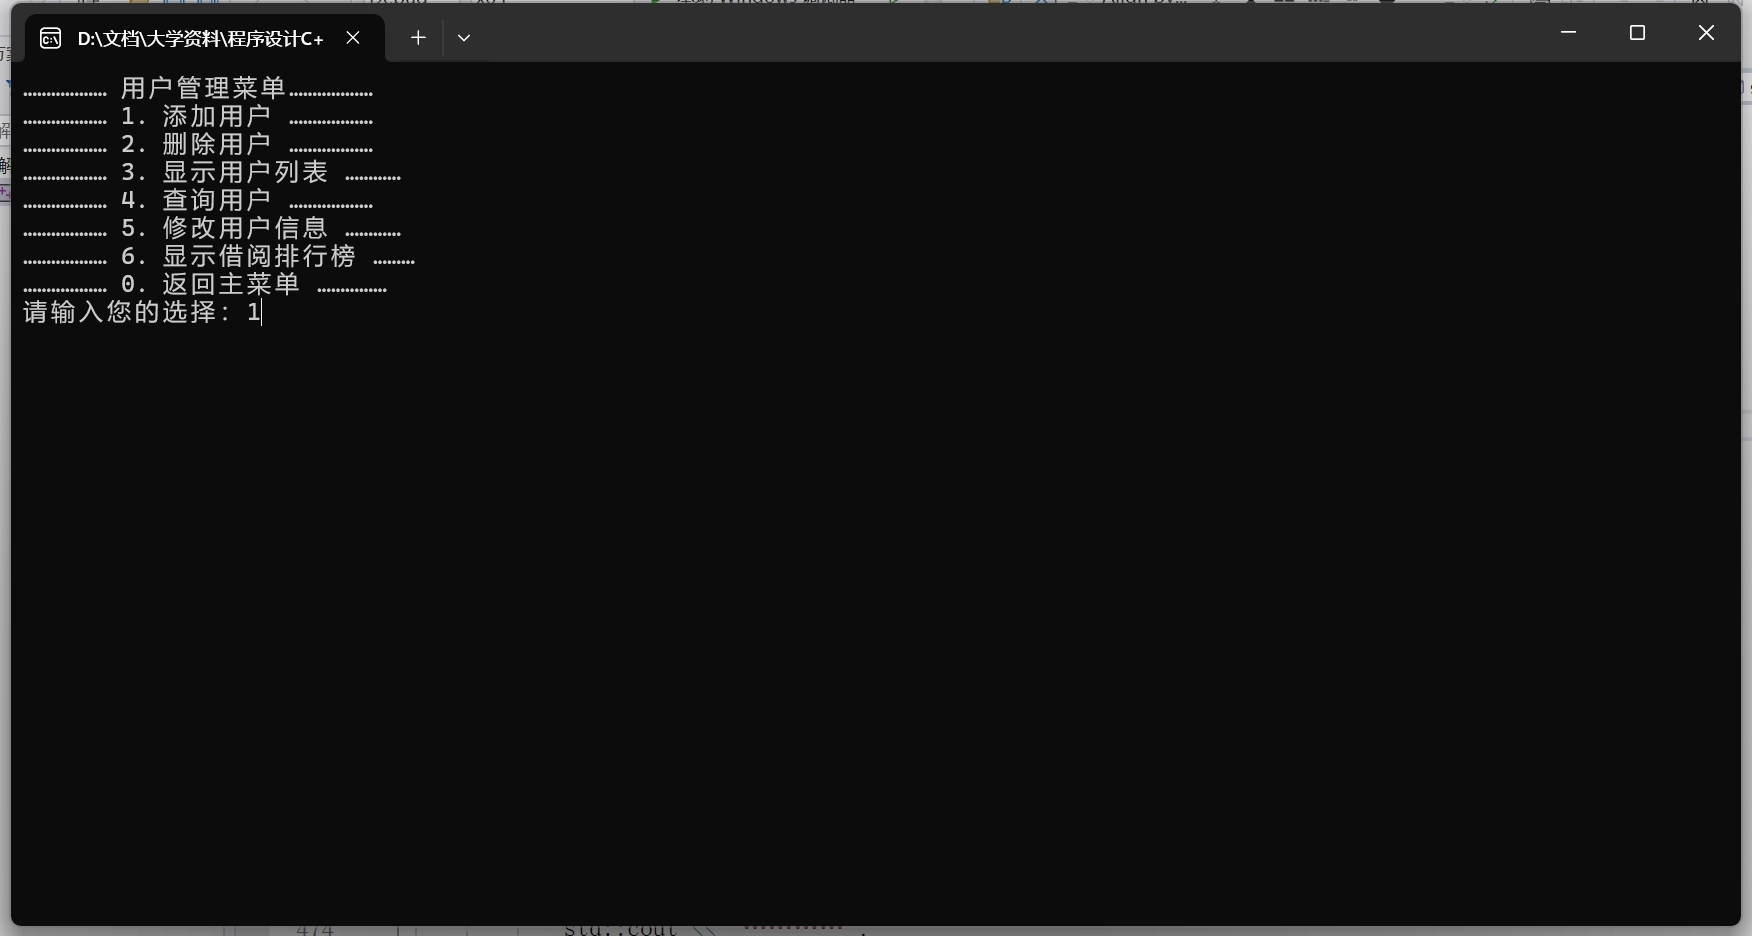
\includegraphics[width=0.8\textwidth]{User1.png}
    \caption{添加用户}
\end{figure}

如果用户添加成功,系统会提示添加成功,如图\ref{fig:AddSucc}、\ref{fig:Addreturn}所示。

\begin{figure}[H]
    \centering
    \begin{minipage}{0.48\textwidth}
        \centering
        \includegraphics[width=\linewidth]{AddUser.png}
        \caption{添加用户成功}
        \label{fig:AddSucc}
    \end{minipage}\hfill
    \begin{minipage}{0.48\textwidth}
        \centering
        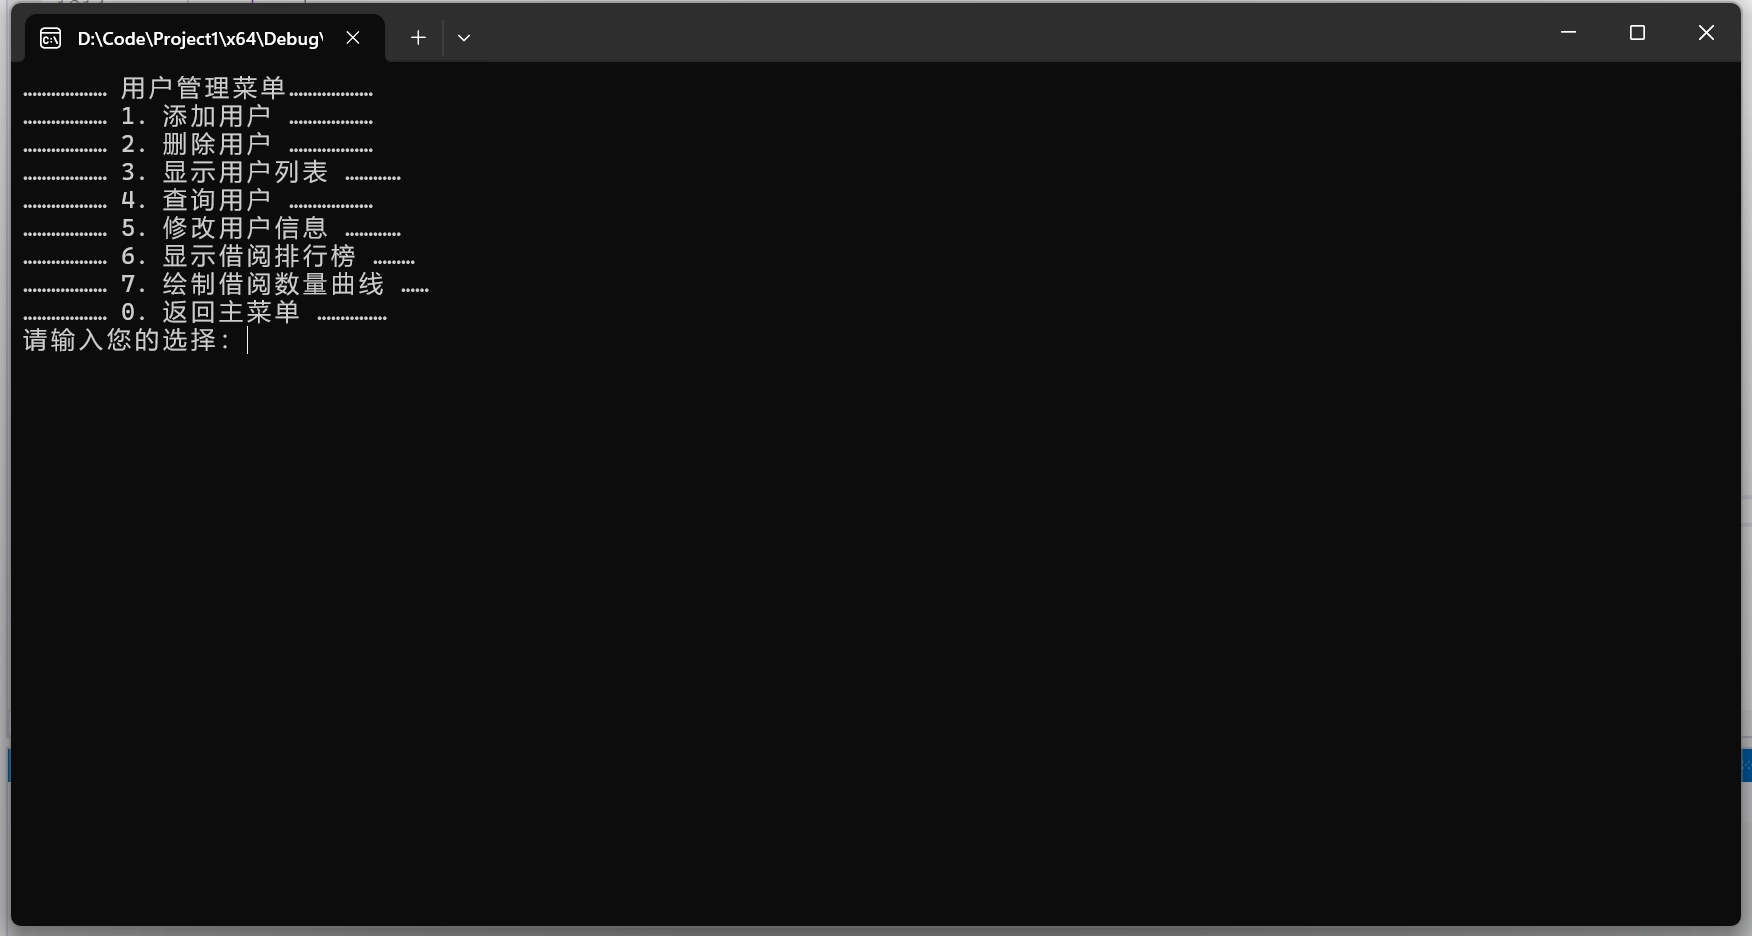
\includegraphics[width=\linewidth]{User.png}
        \caption{返回用户管理界面}
        \label{fig:Addreturn}
    \end{minipage}
\end{figure}

\begin{figure}[H]
    \begin{minipage}[c]{0.5\textwidth}
        $\star$特别地,如果用户名中包含空格,系统依旧可以正常识别,如图\ref{fig:Spaceuser}所
        示,\underline{不必}进行特殊处理。
    \end{minipage}%
    \hfill
    \begin{minipage}[c]{0.45\textwidth}
        \centering
        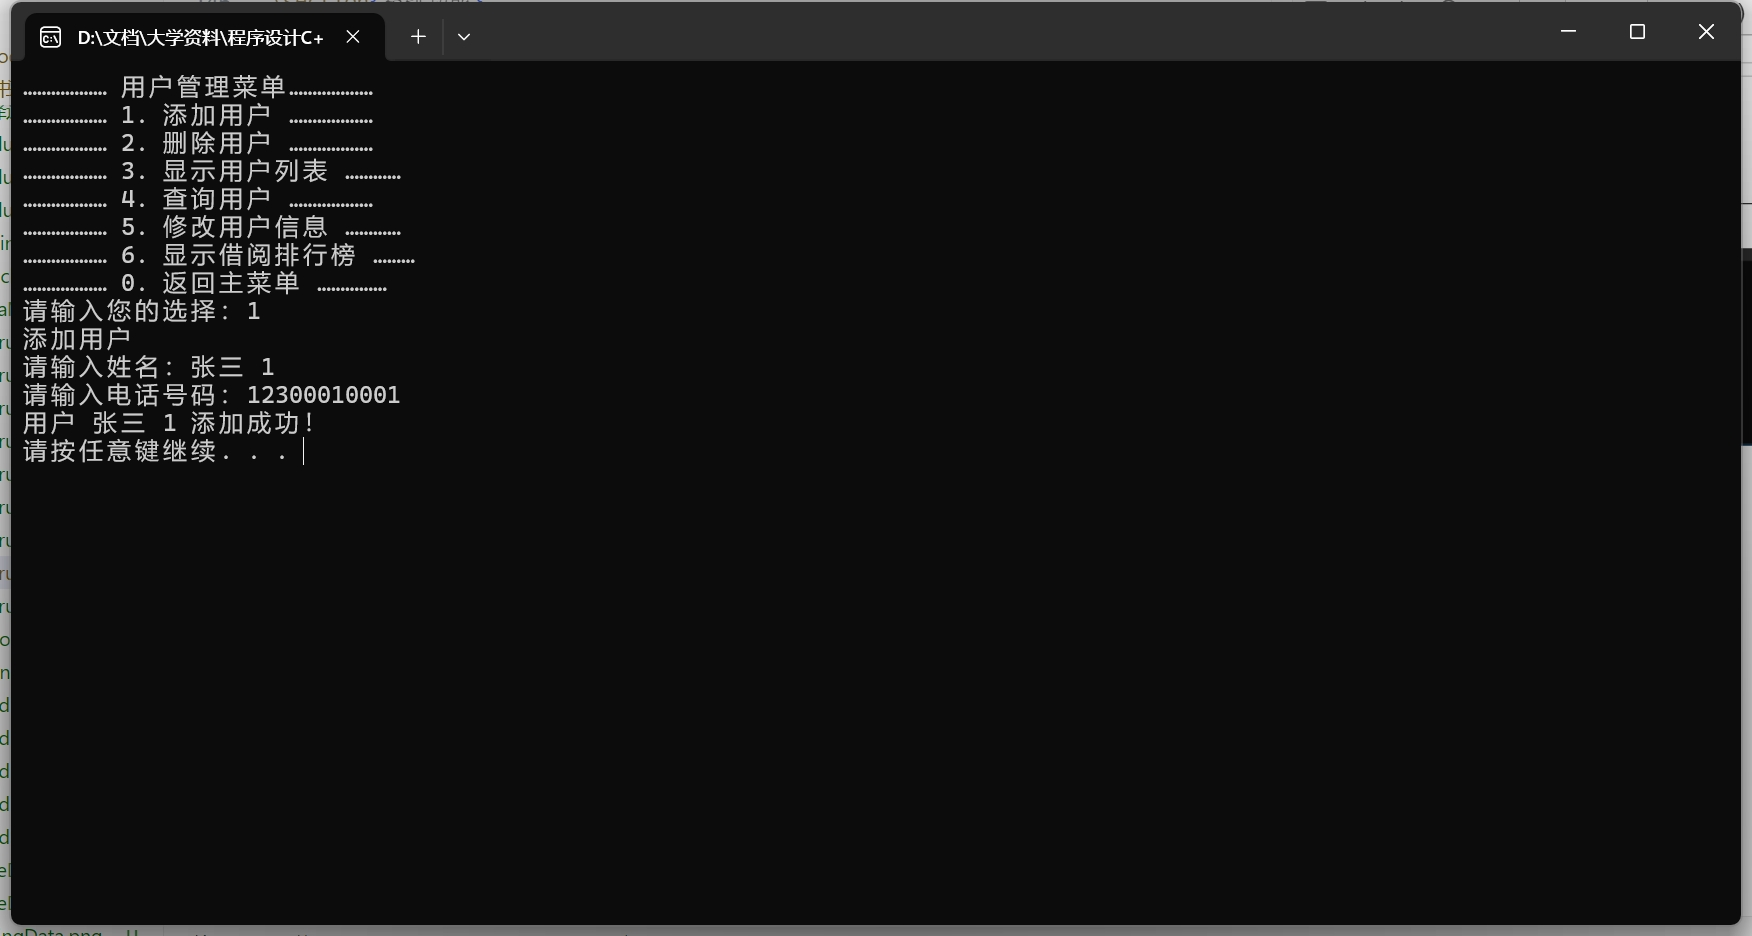
\includegraphics[width=\textwidth]{spaceuser.png}
        \caption{有空格用户名}
        \label{fig:Spaceuser}
    \end{minipage}
\end{figure}

如果用户添加失败,系统会提示添加失败,如图\ref{fig:Addusererror}所示,
可能是因为手机号输入有误,用户可以重新输入,如图\ref{fig:Adduseragain}所示。
\begin{figure}[H]
    \begin{minipage}[c]{0.48\textwidth}
        \centering
        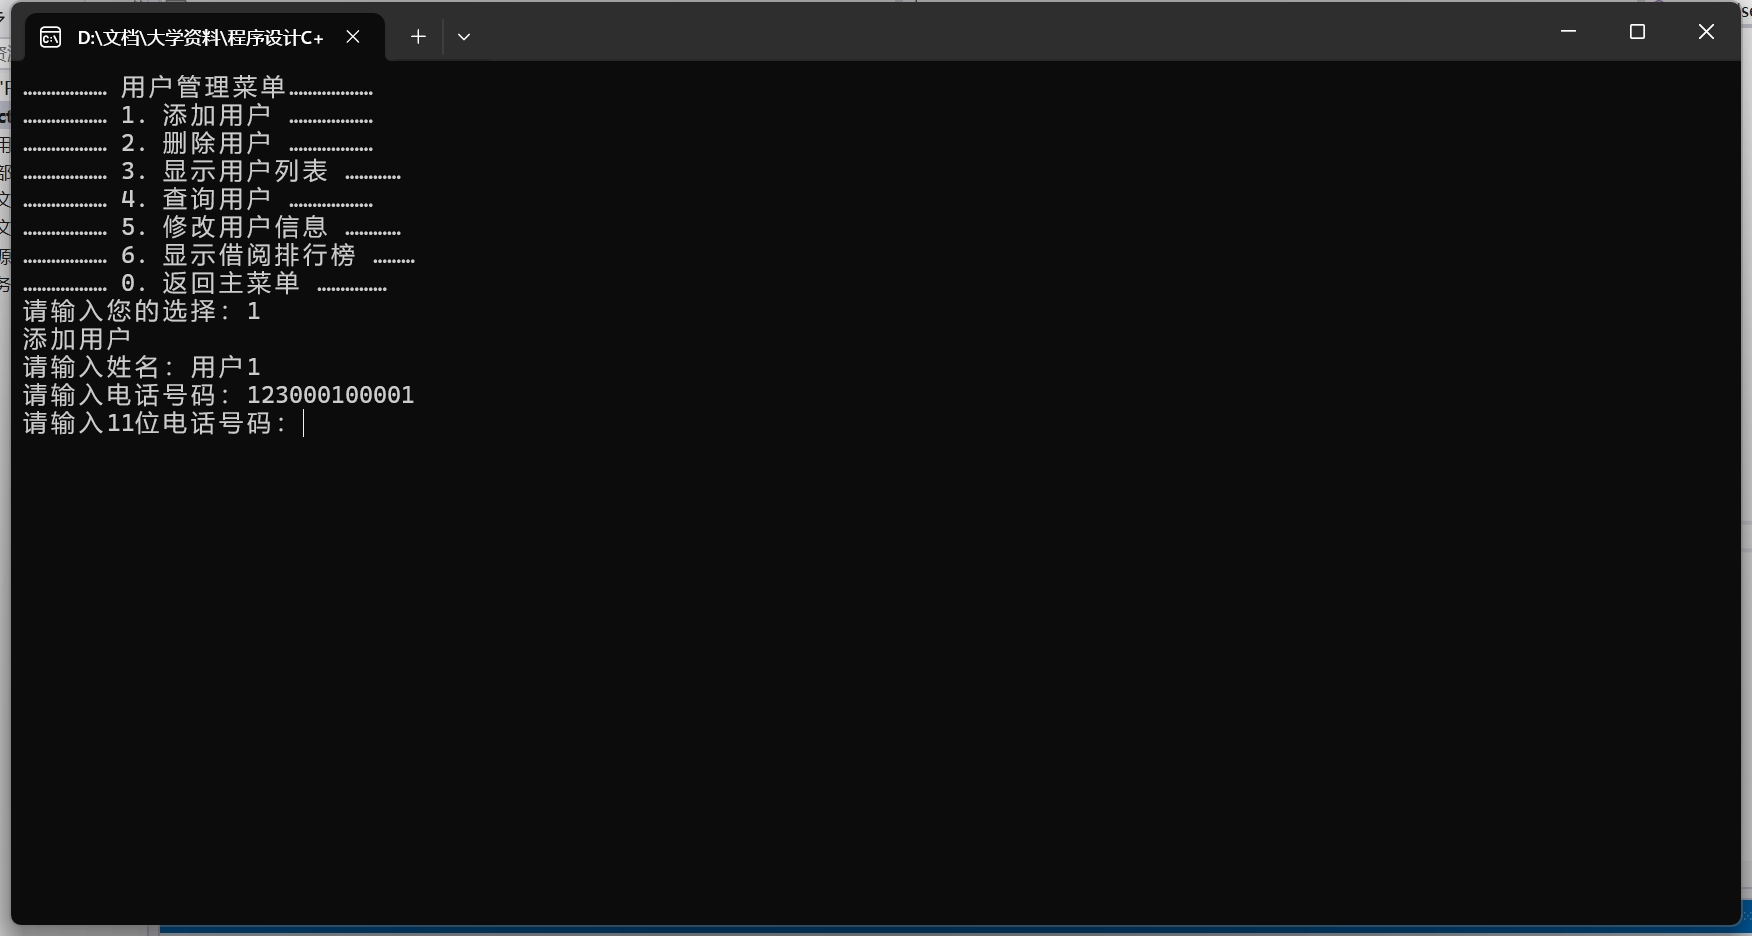
\includegraphics[width=\textwidth]{Addusererror.png}
        \caption{手机号输入有误}
        \label{fig:Addusererror}
    \end{minipage}
    \hfill
    \begin{minipage}[c]{0.48\textwidth}
        \centering
        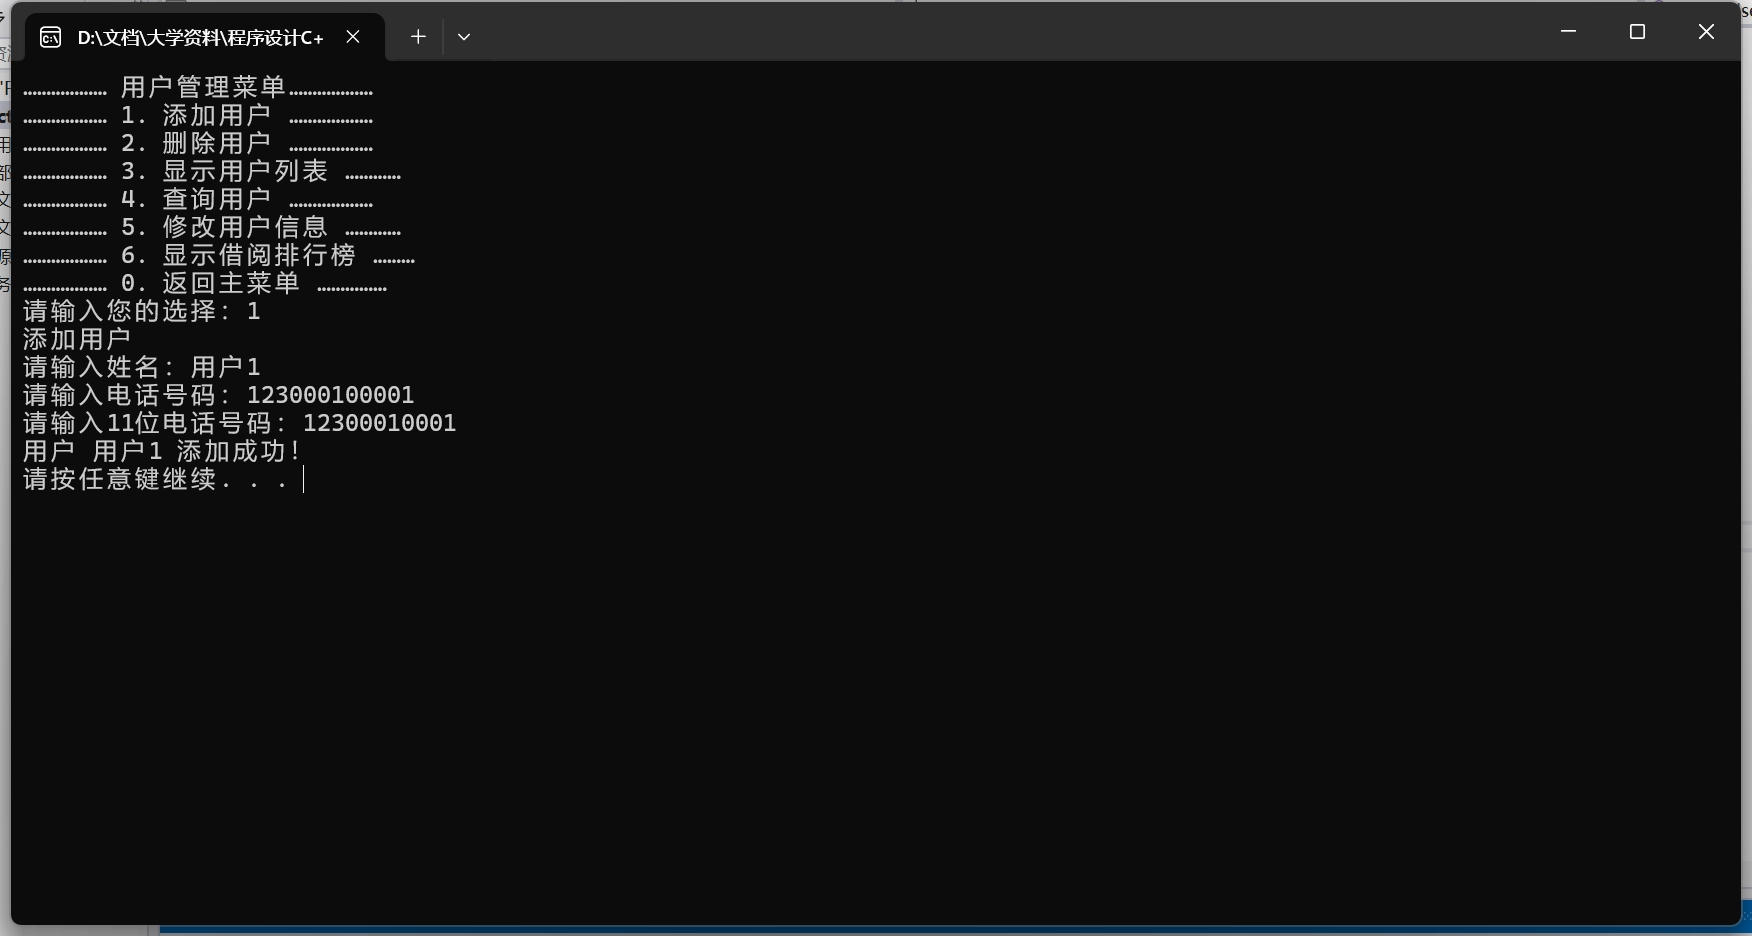
\includegraphics[width=\textwidth]{Adduseragain.png}
        \caption{重新输入}
        \label{fig:Adduseragain}
    \end{minipage}
\end{figure}

\subsubsection{删除用户}
\begin{figure}[H]
    \centering
    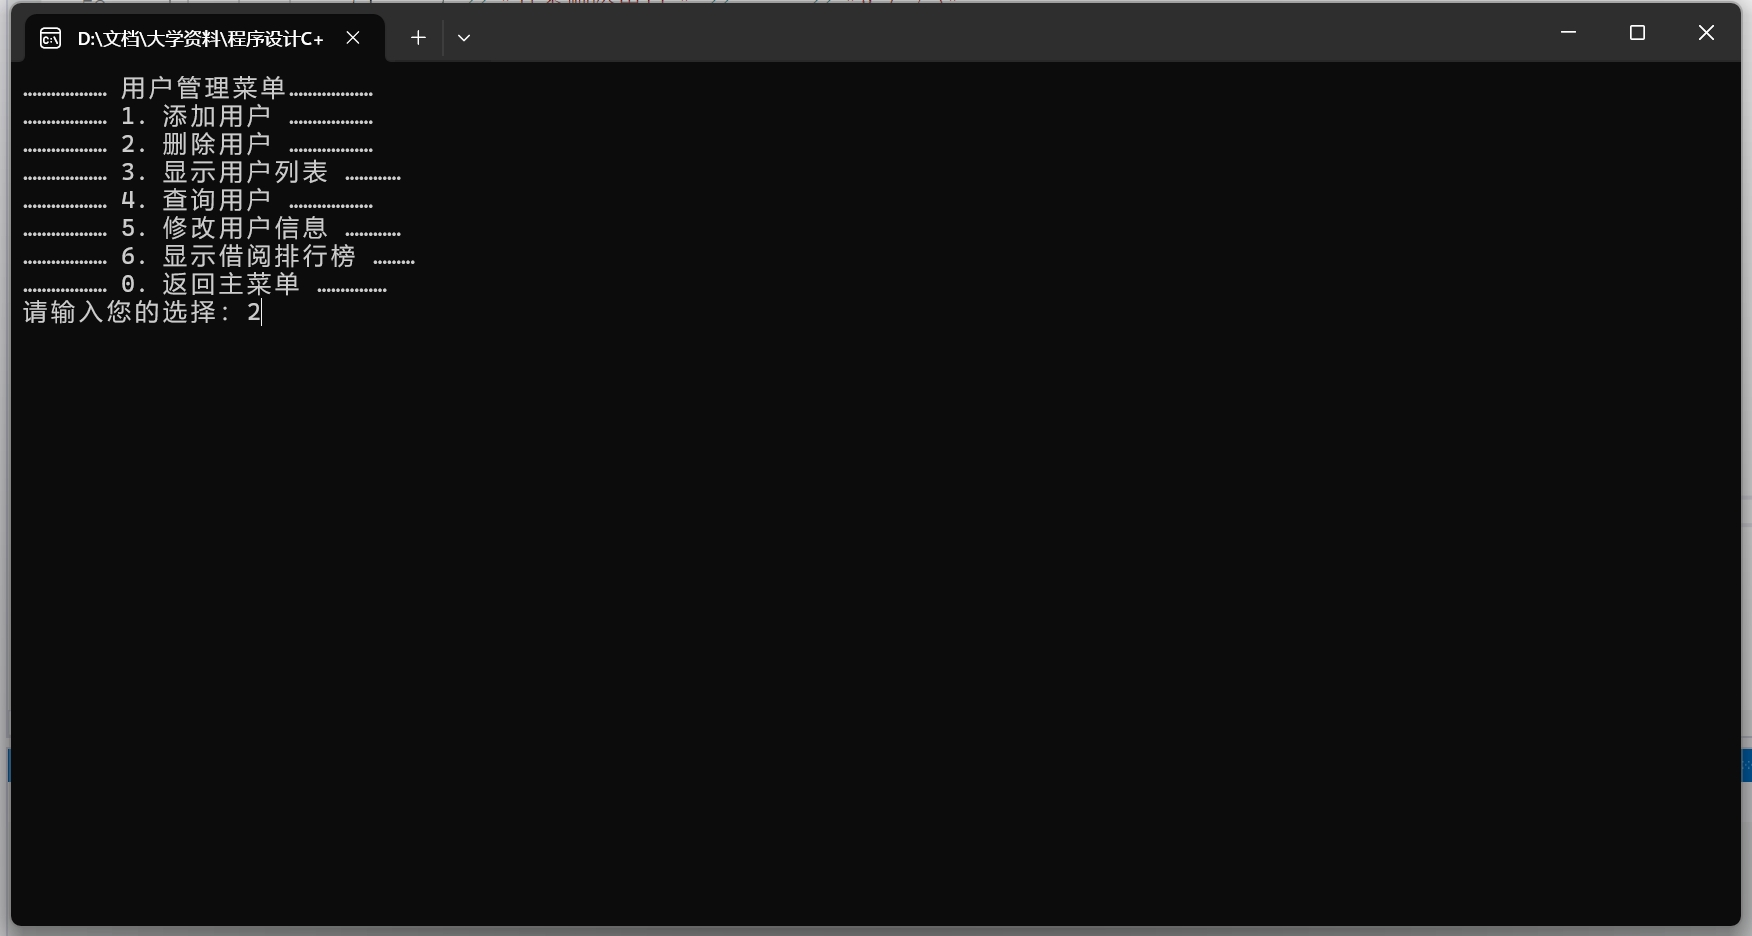
\includegraphics[width=0.8\textwidth]{Delete.png}
    \caption{删除用户}
\end{figure}

\begin{figure}[H]
    \centering
    \includegraphics[width=0.8\textwidth]{DeleteUser.png}
    \caption{删除用户界面}
\end{figure}

删除用户时,用户输入要删除的用户名称,系统会提示是否确认删除,
如图\ref{fig:confirmdeleteuser},如果确认删除,按提示输入后,
如图\ref{fig:Deleteuserconfirm}
系统会提示删除成功,如图\ref{fig:DeleteSucc}、\ref{fig:DeleteReturn}所示。
\begin{figure}[H]
    \centering
    \begin{minipage}{0.48\textwidth}
        \centering
        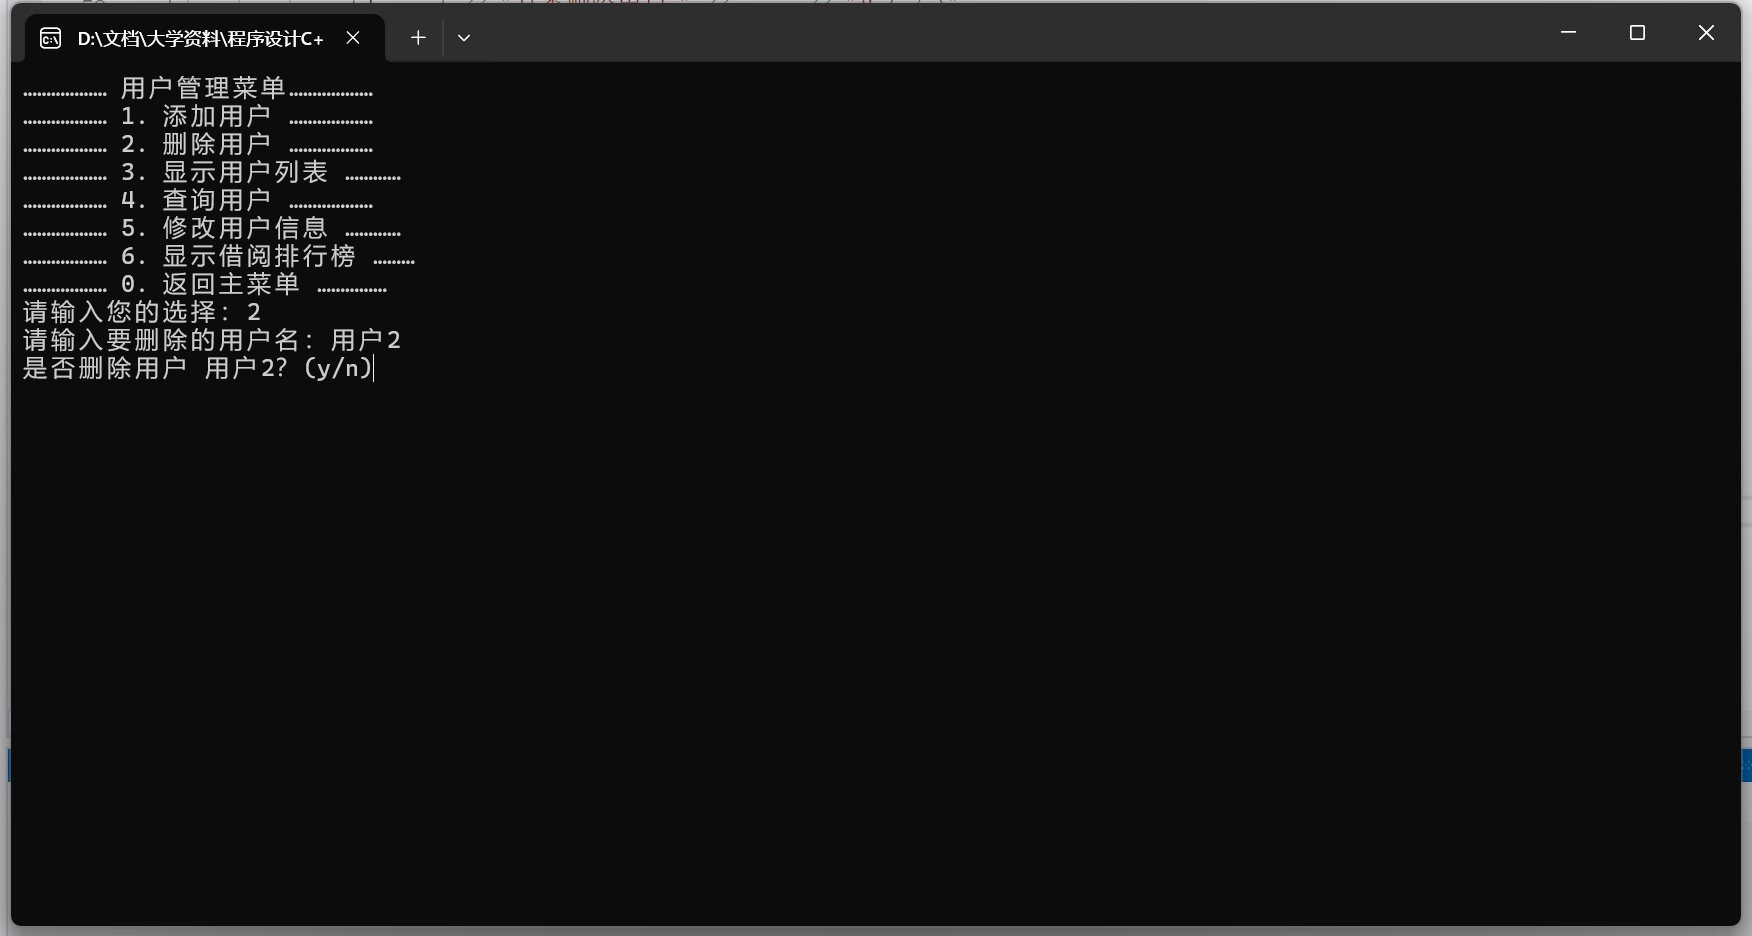
\includegraphics[width=\linewidth]{confirmdeleteuser.png}
        \caption{确认是否删除}
        \label{fig:confirmdeleteuser}
    \end{minipage}\hfill
    \begin{minipage}{0.48\textwidth}
        \centering
        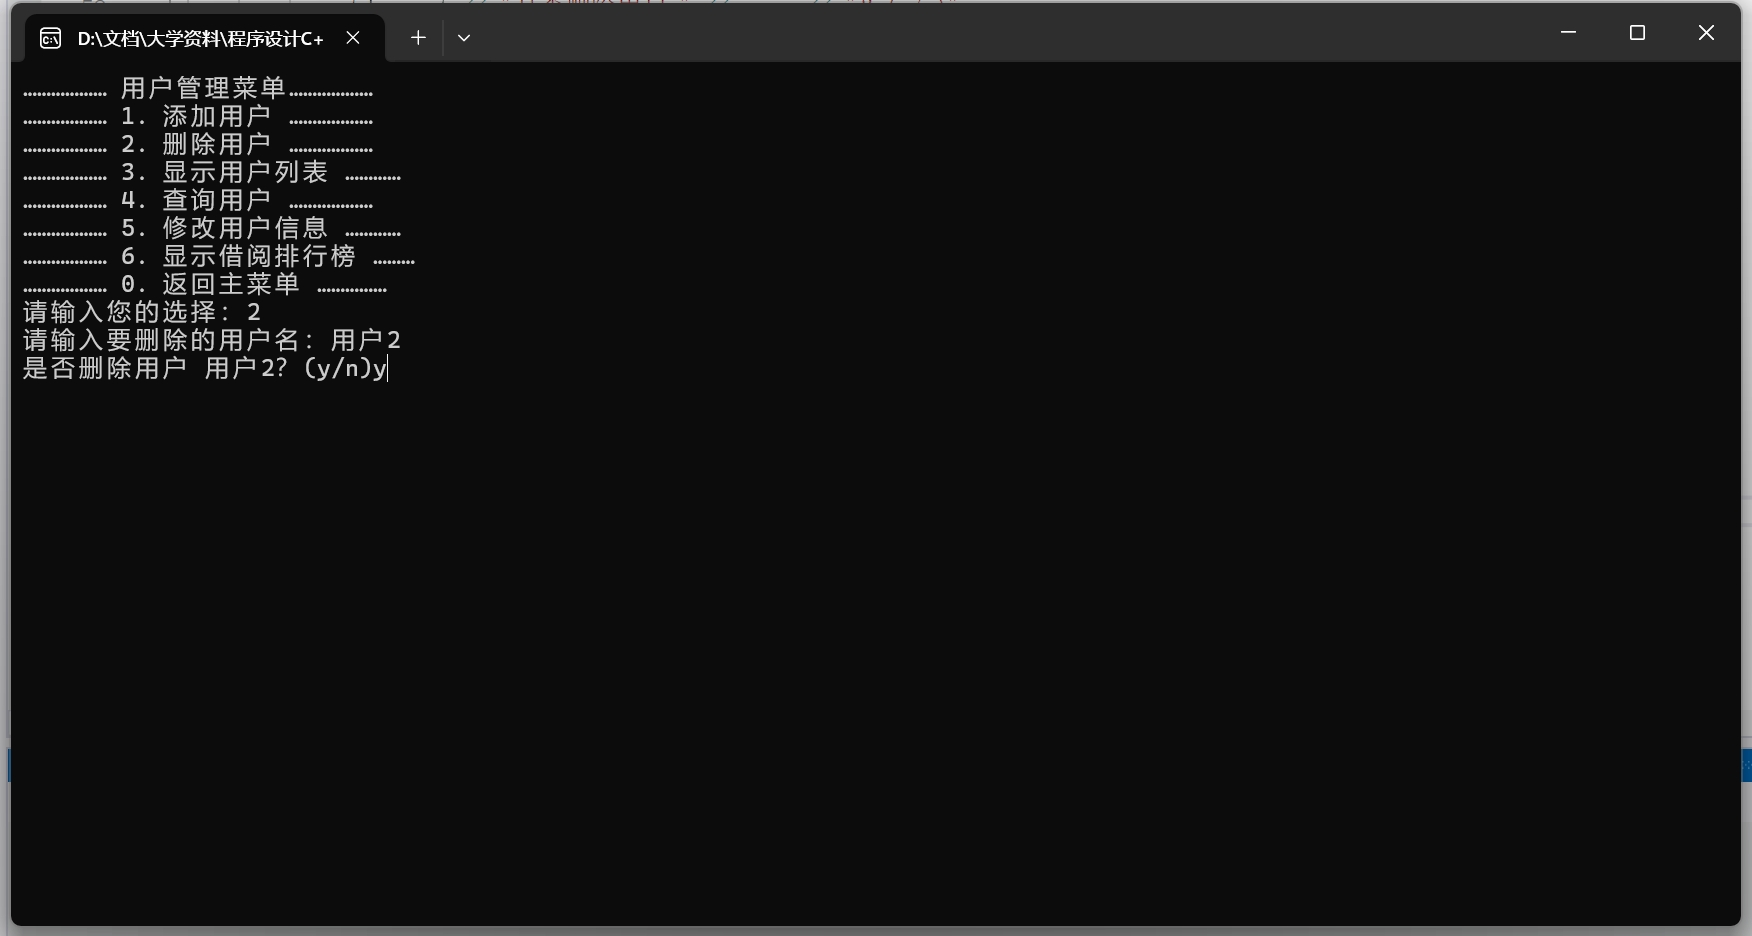
\includegraphics[width=\linewidth]{Deleteuserconfirm.png}
        \caption{用户确认删除}
        \label{fig:Deleteuserconfirm}
    \end{minipage}
\end{figure}
\begin{figure}[H]
    \centering
    \begin{minipage}{0.48\textwidth}
        \centering
        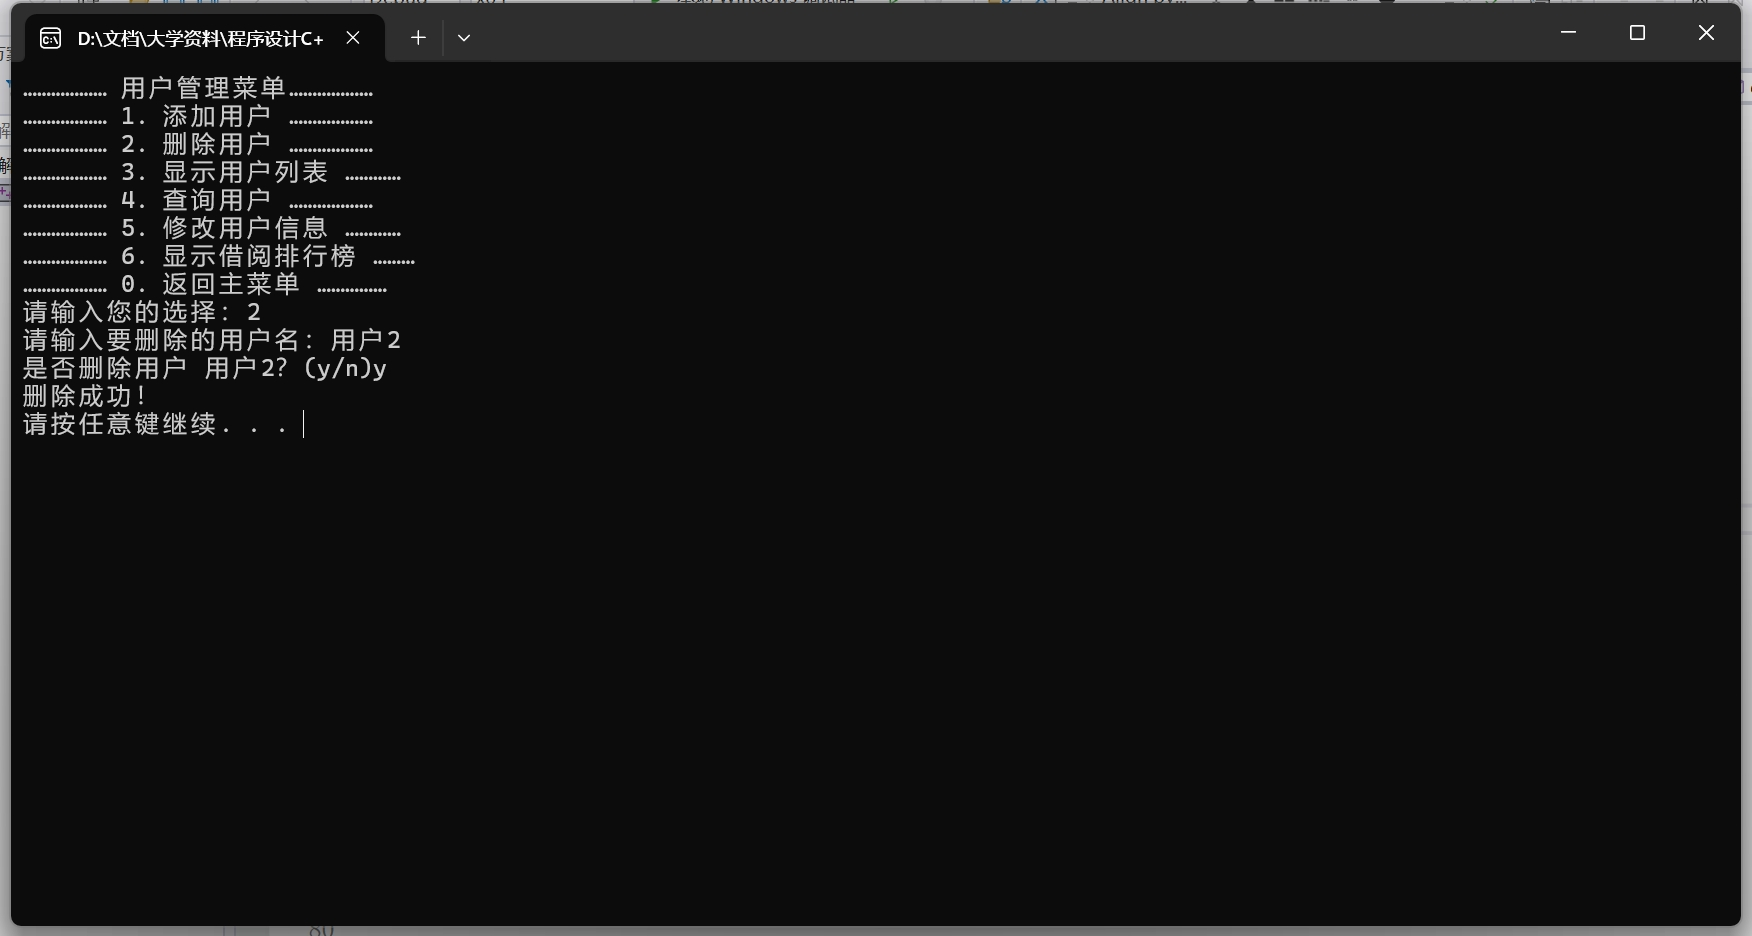
\includegraphics[width=\linewidth]{deleteusersucc.png}
        \caption{删除成功}
        \label{fig:DeleteSucc}
    \end{minipage}\hfill
    \begin{minipage}{0.48\textwidth}
        \centering
        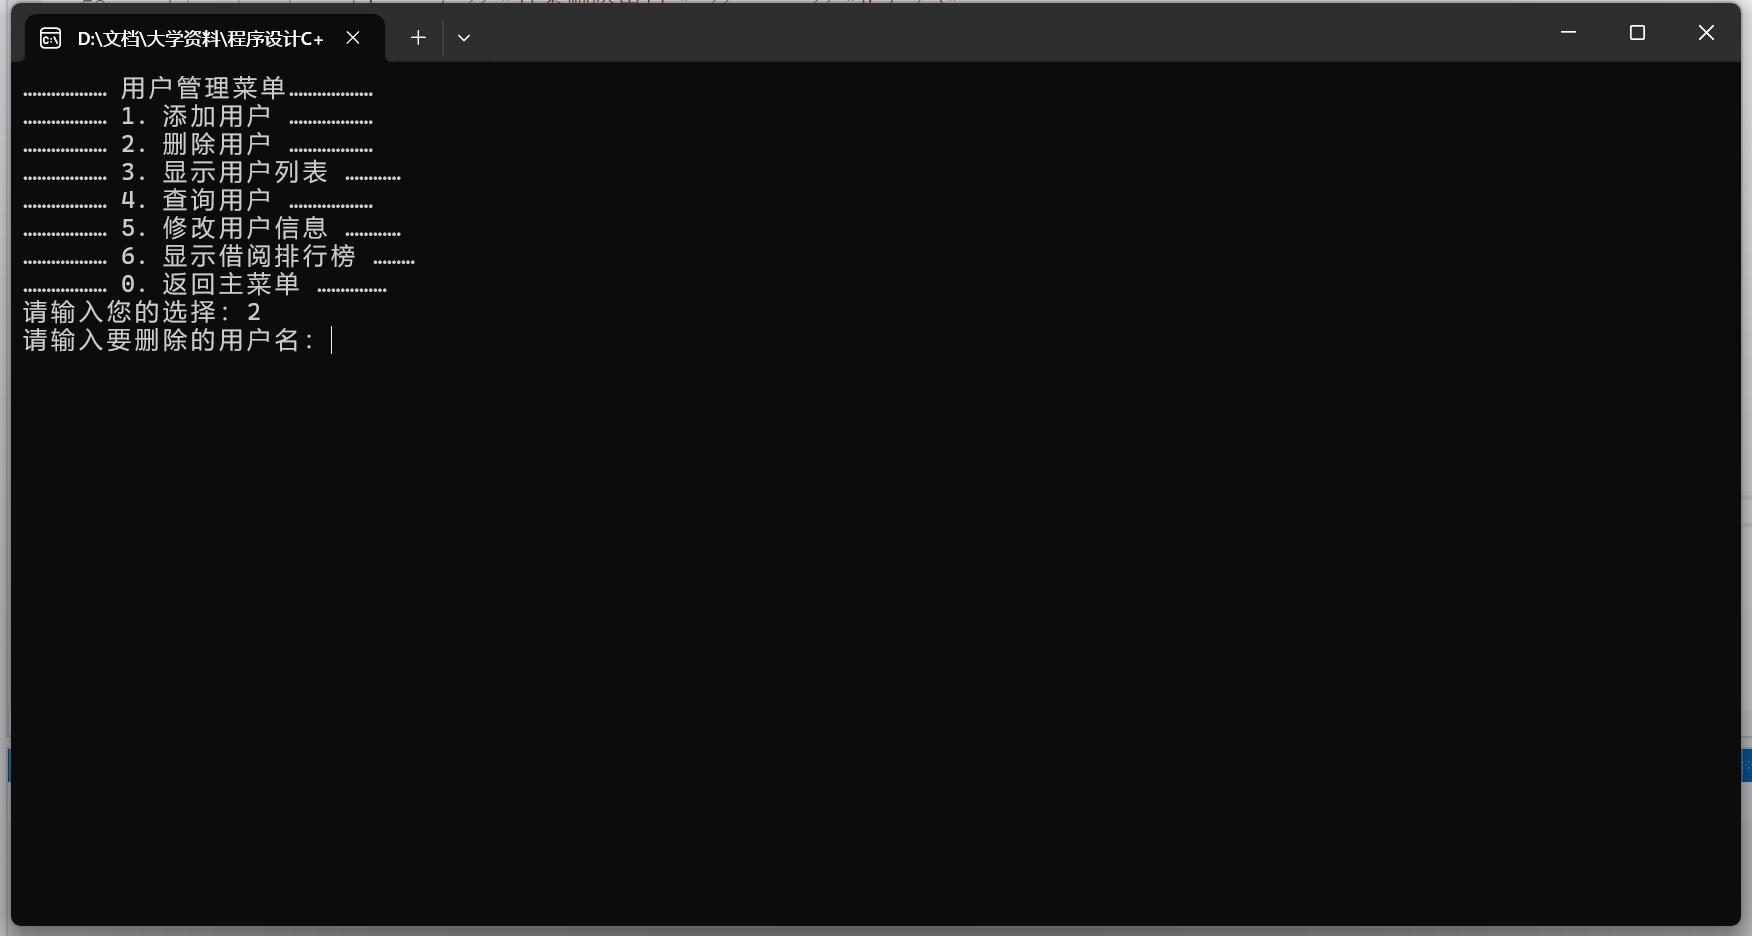
\includegraphics[width=\linewidth]{Deleteuser.png}
        \caption{返回用户管理界面}
        \label{fig:DeleteReturn}
    \end{minipage}
\end{figure}

如果用户取消删除,在系统提示是否确认删除时,如图\ref{fig:nodeleteuser}按要求输入后
会提示取消删除成功,如图\ref{fig:nodeleteusers}所示。

\begin{figure}[H]
    \centering
    \begin{minipage}{0.48\textwidth}
        \centering
        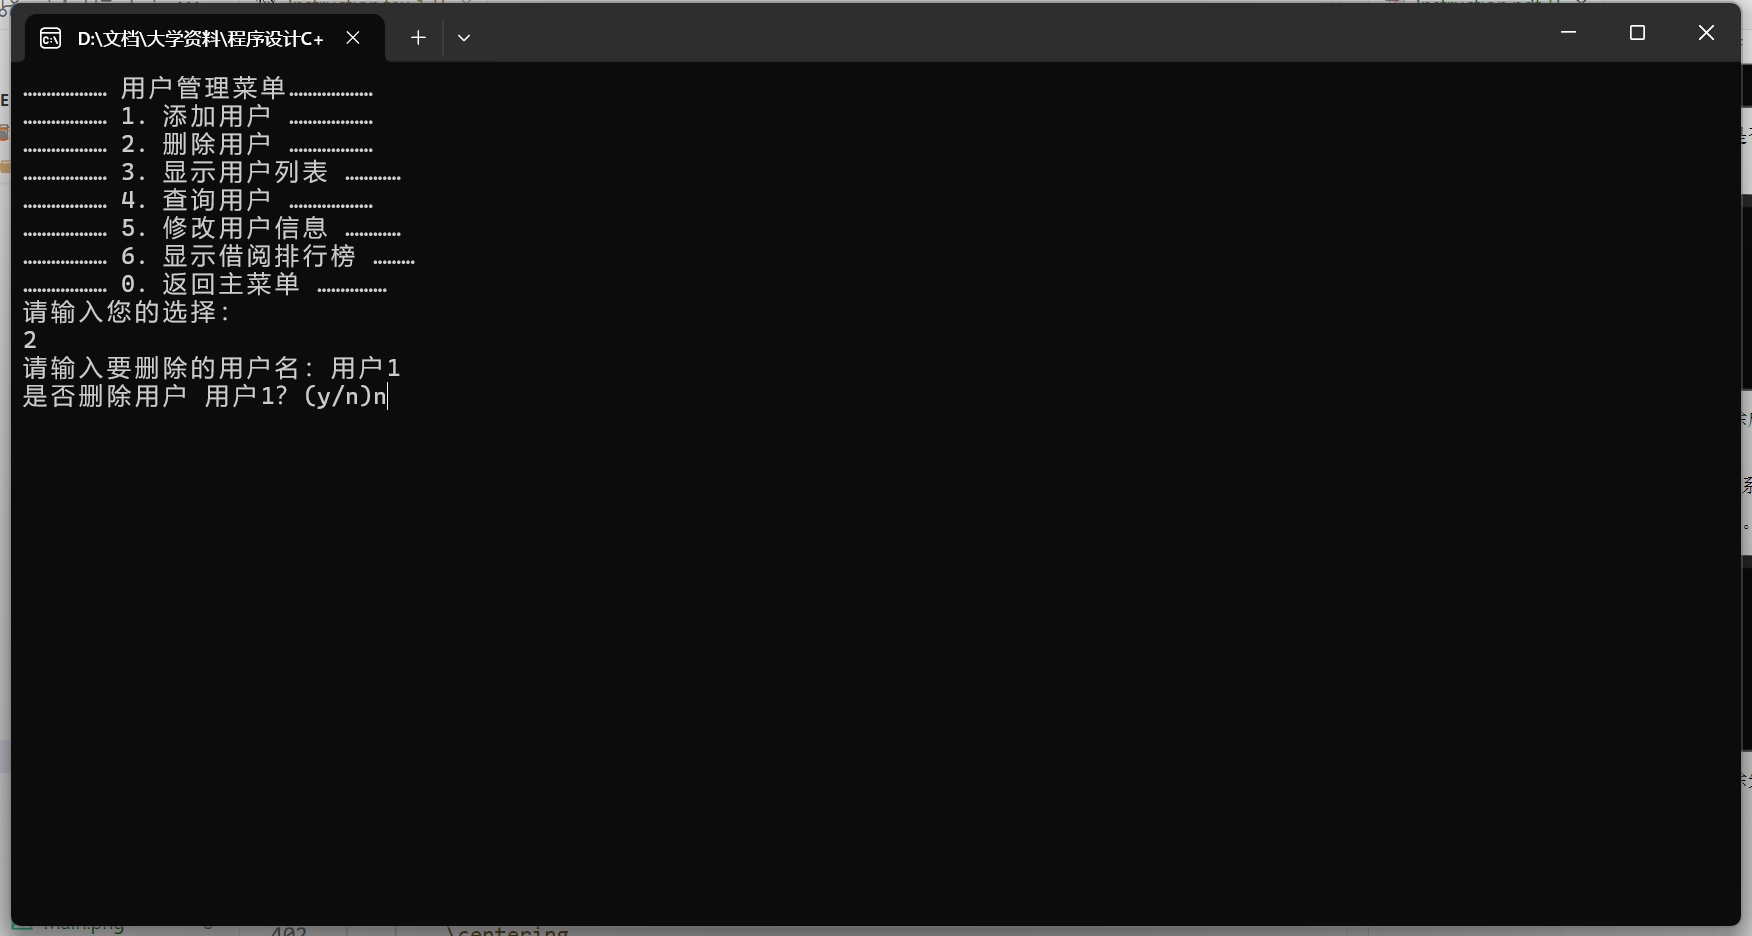
\includegraphics[width=\linewidth]{nodeleteuser.png}
        \caption{取消删除}
        \label{fig:nodeleteuser}
    \end{minipage}\hfill
    \begin{minipage}{0.48\textwidth}
        \centering
        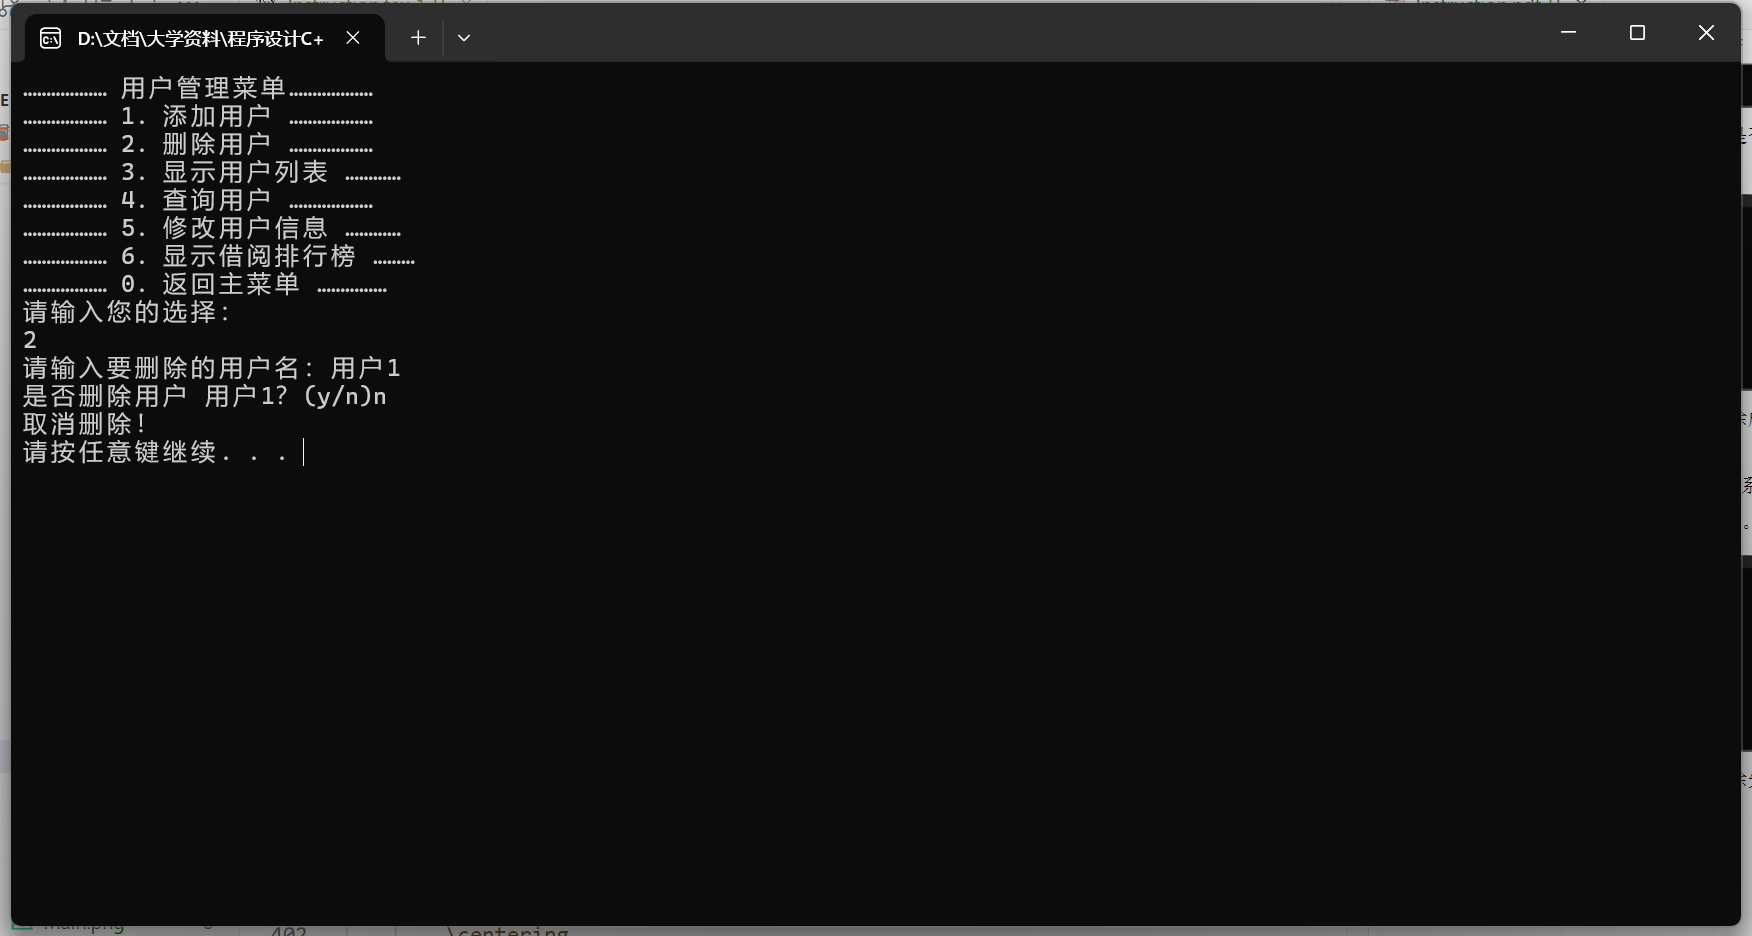
\includegraphics[width=\linewidth]{nodeleteusers.png}
        \caption{取消删除成功}
        \label{fig:nodeleteusers}
    \end{minipage}
\end{figure}

如果用户删除失败,系统会提示删除失败,如图\ref{fig:DeleteFailed}所示,
可能是因为用户不存在,用户可以重新输入,如图\ref{fig:DeleteAgain}所示。

\begin{figure}[H]
    \begin{minipage}[c]{0.48\textwidth}
        \centering
        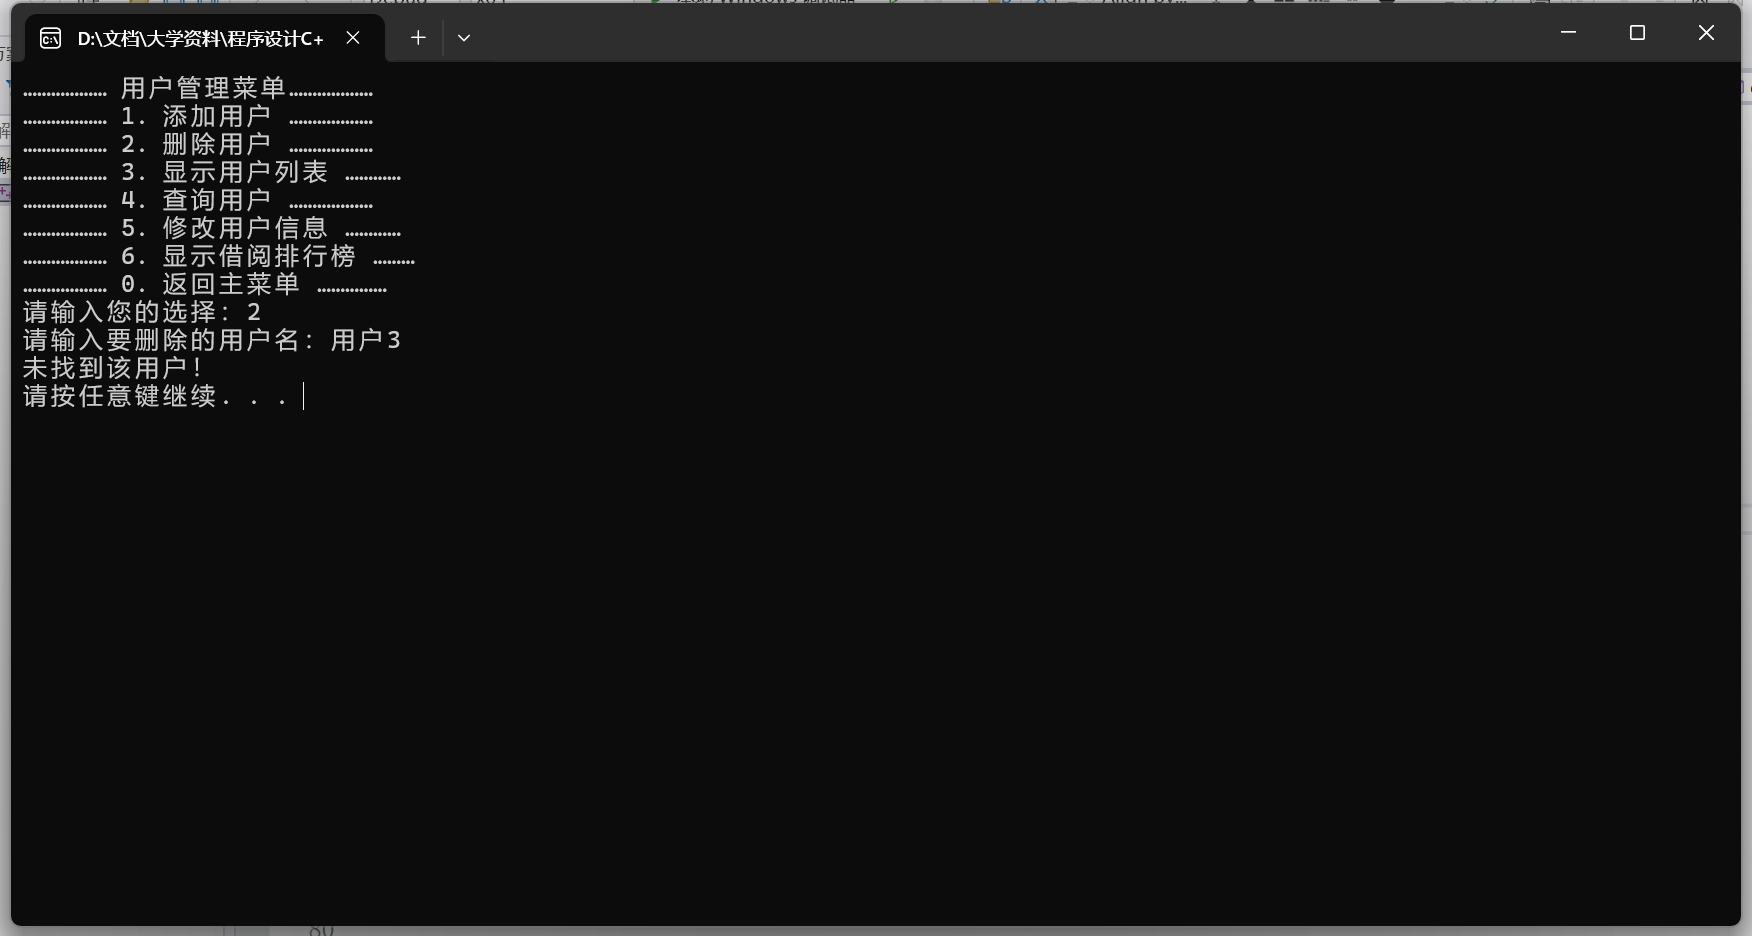
\includegraphics[width=\textwidth]{deleteuserfail.png}
        \caption{删除失败}
        \label{fig:DeleteFailed}
    \end{minipage}
    \hfill
    \begin{minipage}[c]{0.48\textwidth}
        \centering
        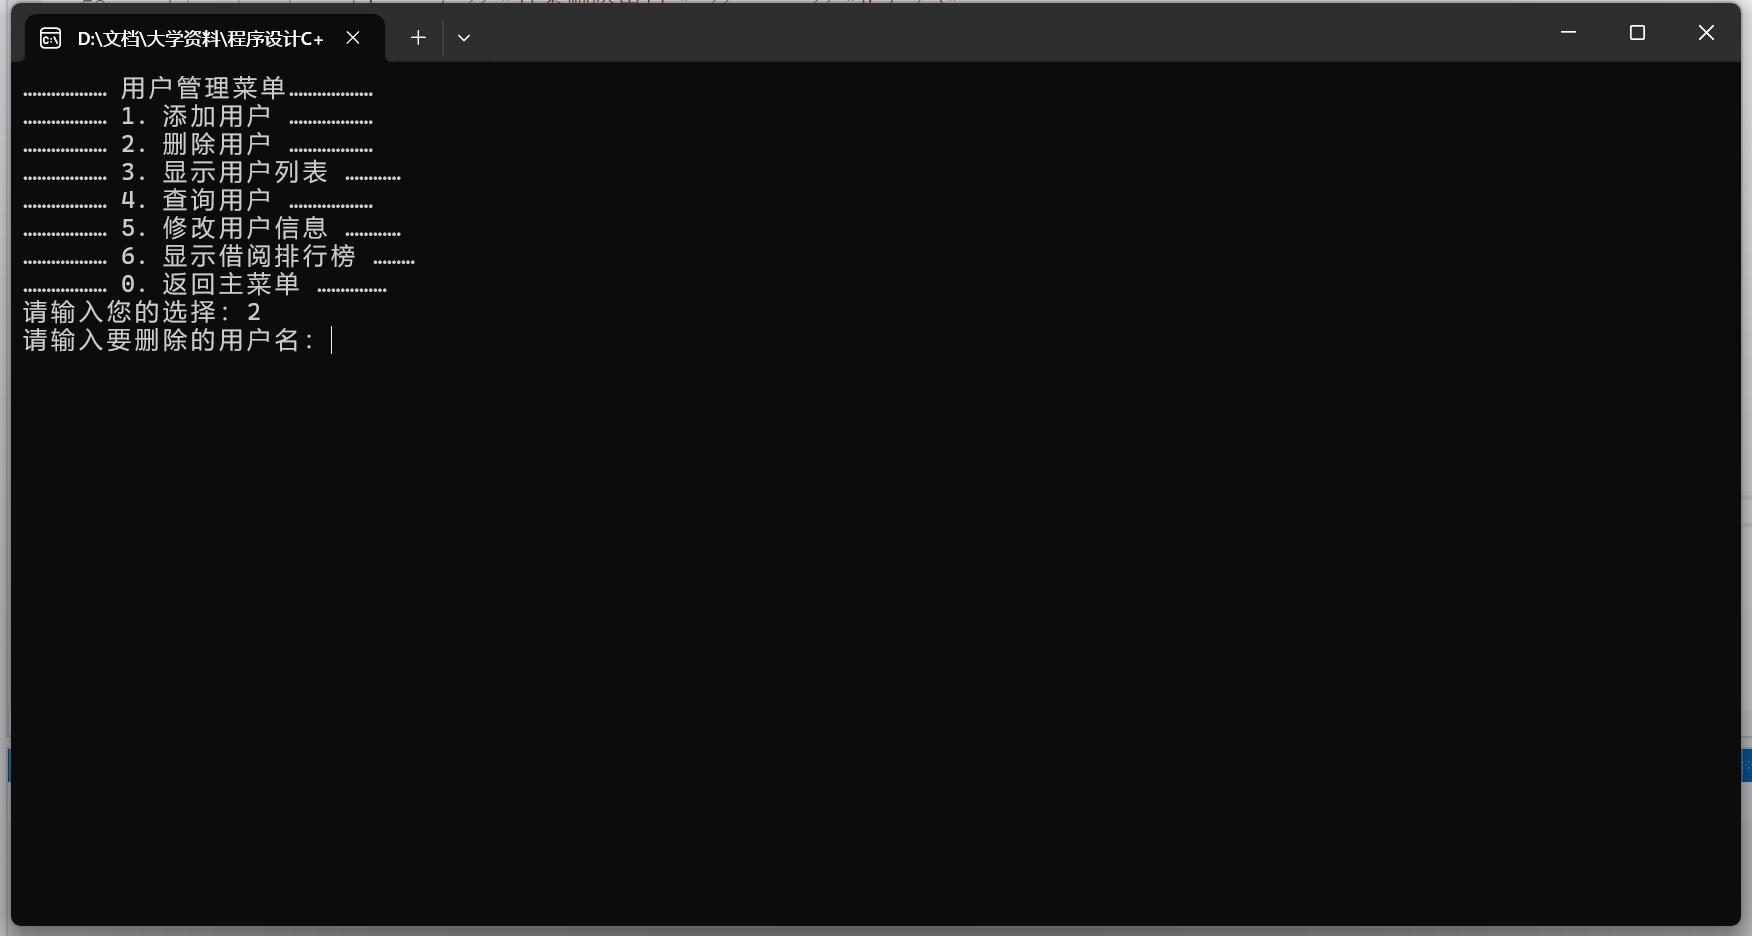
\includegraphics[width=\textwidth]{Deleteuser.png}
        \caption{重新输入}
        \label{fig:DeleteAgain}
    \end{minipage}
\end{figure}

\subsubsection{显示用户列表}

\begin{figure}[H]
    \centering
    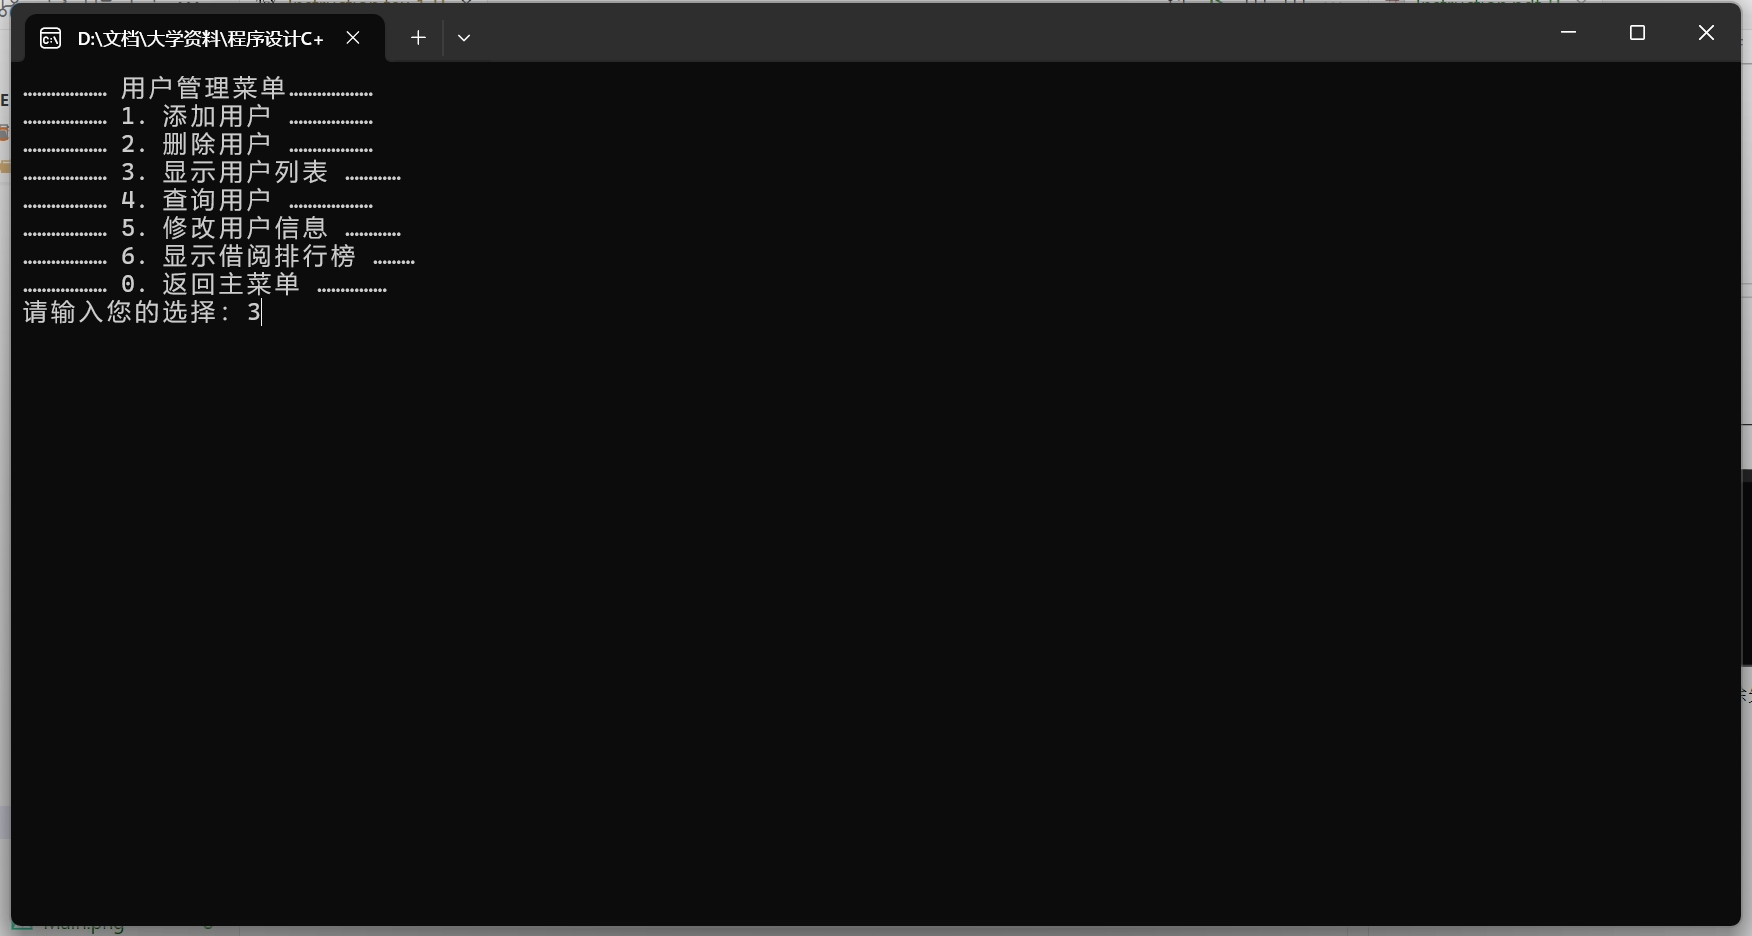
\includegraphics[width=0.8\textwidth]{selectuserlist.png}
    \caption{选择显示用户列表}
\end{figure}

\begin{figure}[H]
    \centering
    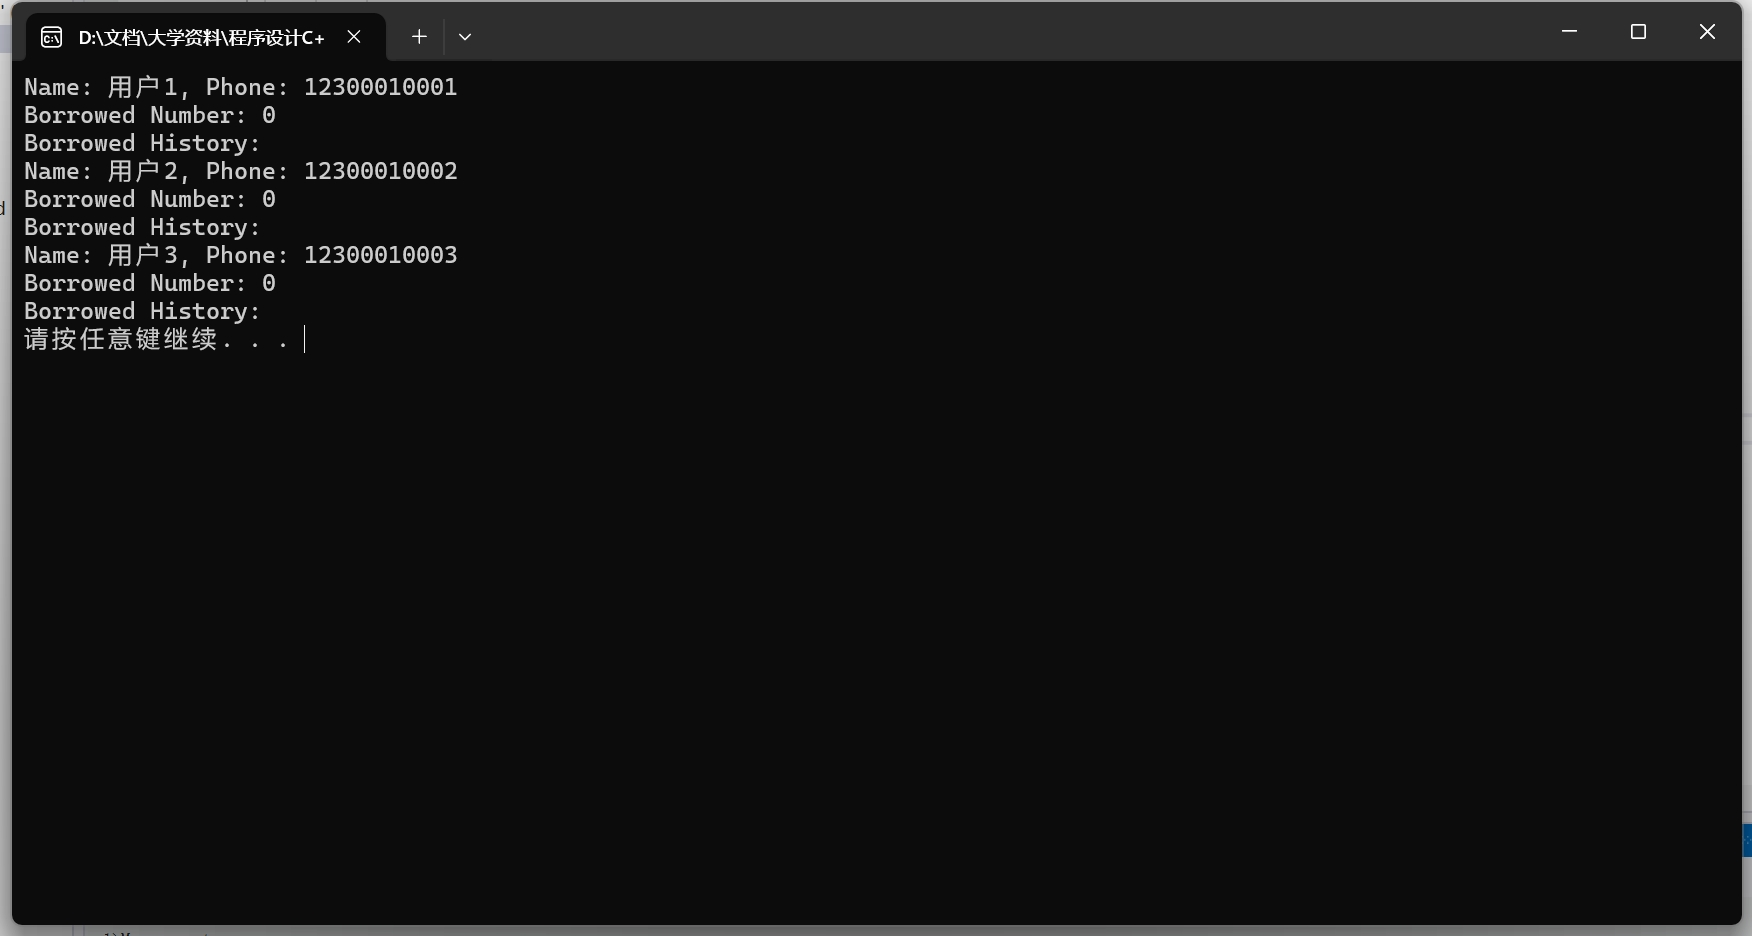
\includegraphics[width=0.8\textwidth]{showusers.png}
    \caption{显示用户列表}
\end{figure}

\subsubsection{查找用户}

\begin{figure}[H]
    \centering
    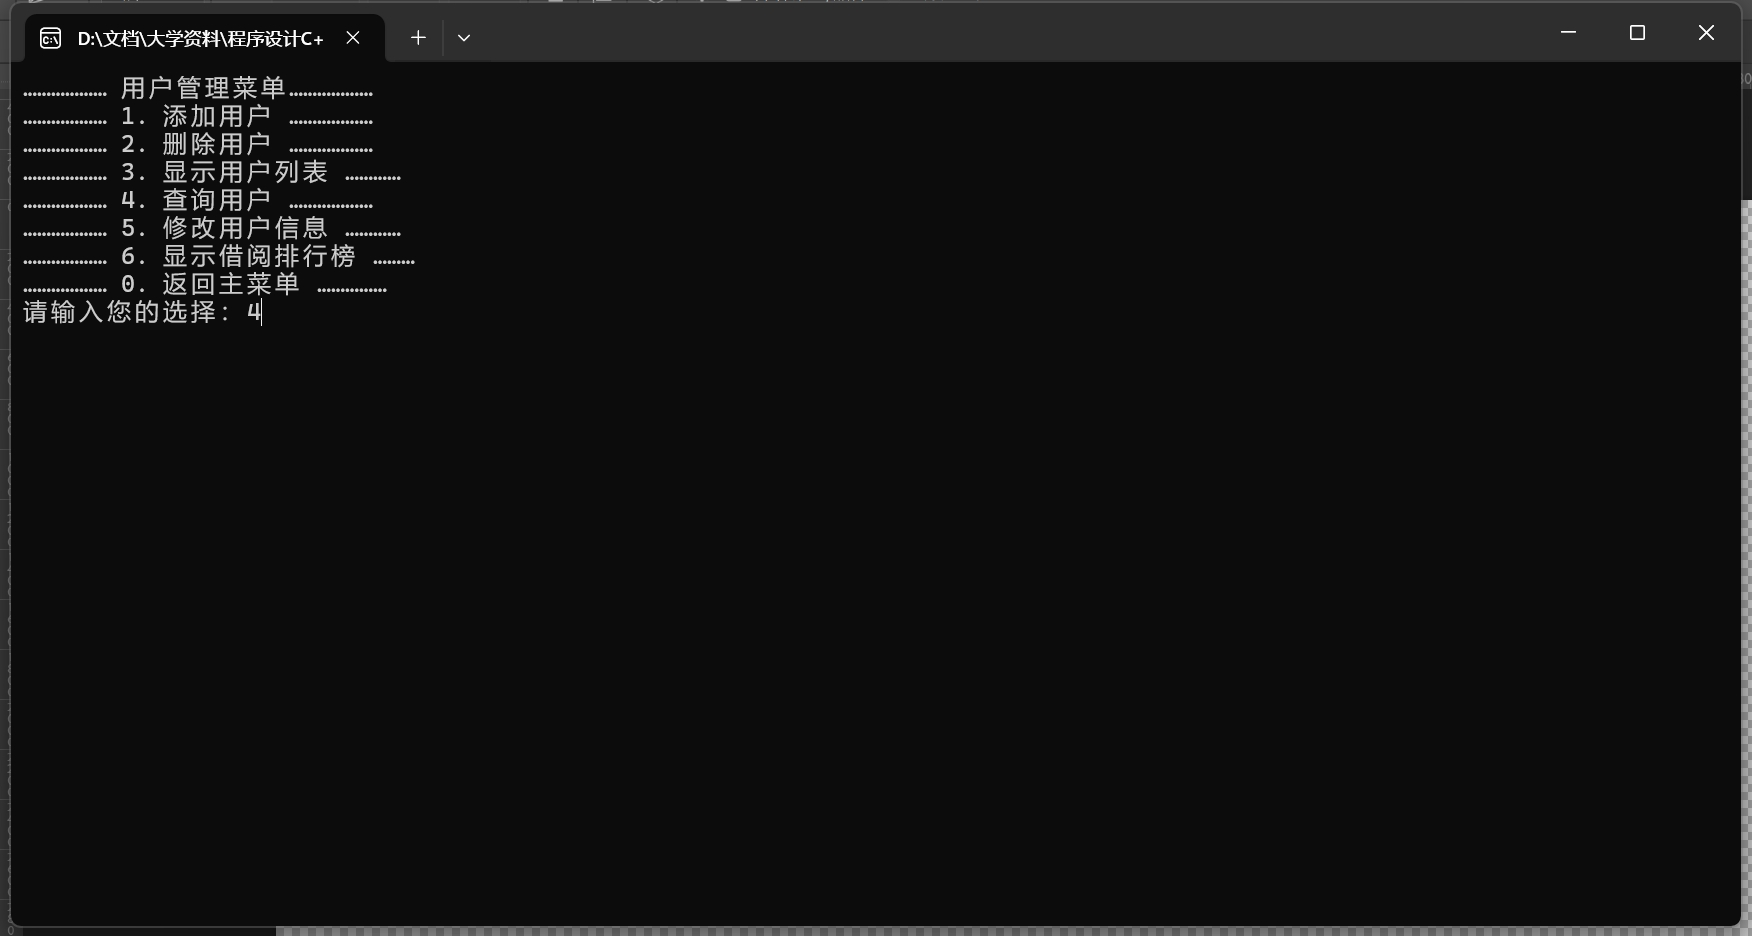
\includegraphics[width=0.8\textwidth]{selectsearchuser.png}
    \caption{选择查找用户}
\end{figure}

按照如图\ref{fig:searchuser}提示输入需要查找的用户名称,系统会显示查找到的用户信息,
如图\ref{fig:searchresult}所示。
\begin{figure}[H]
    \centering
    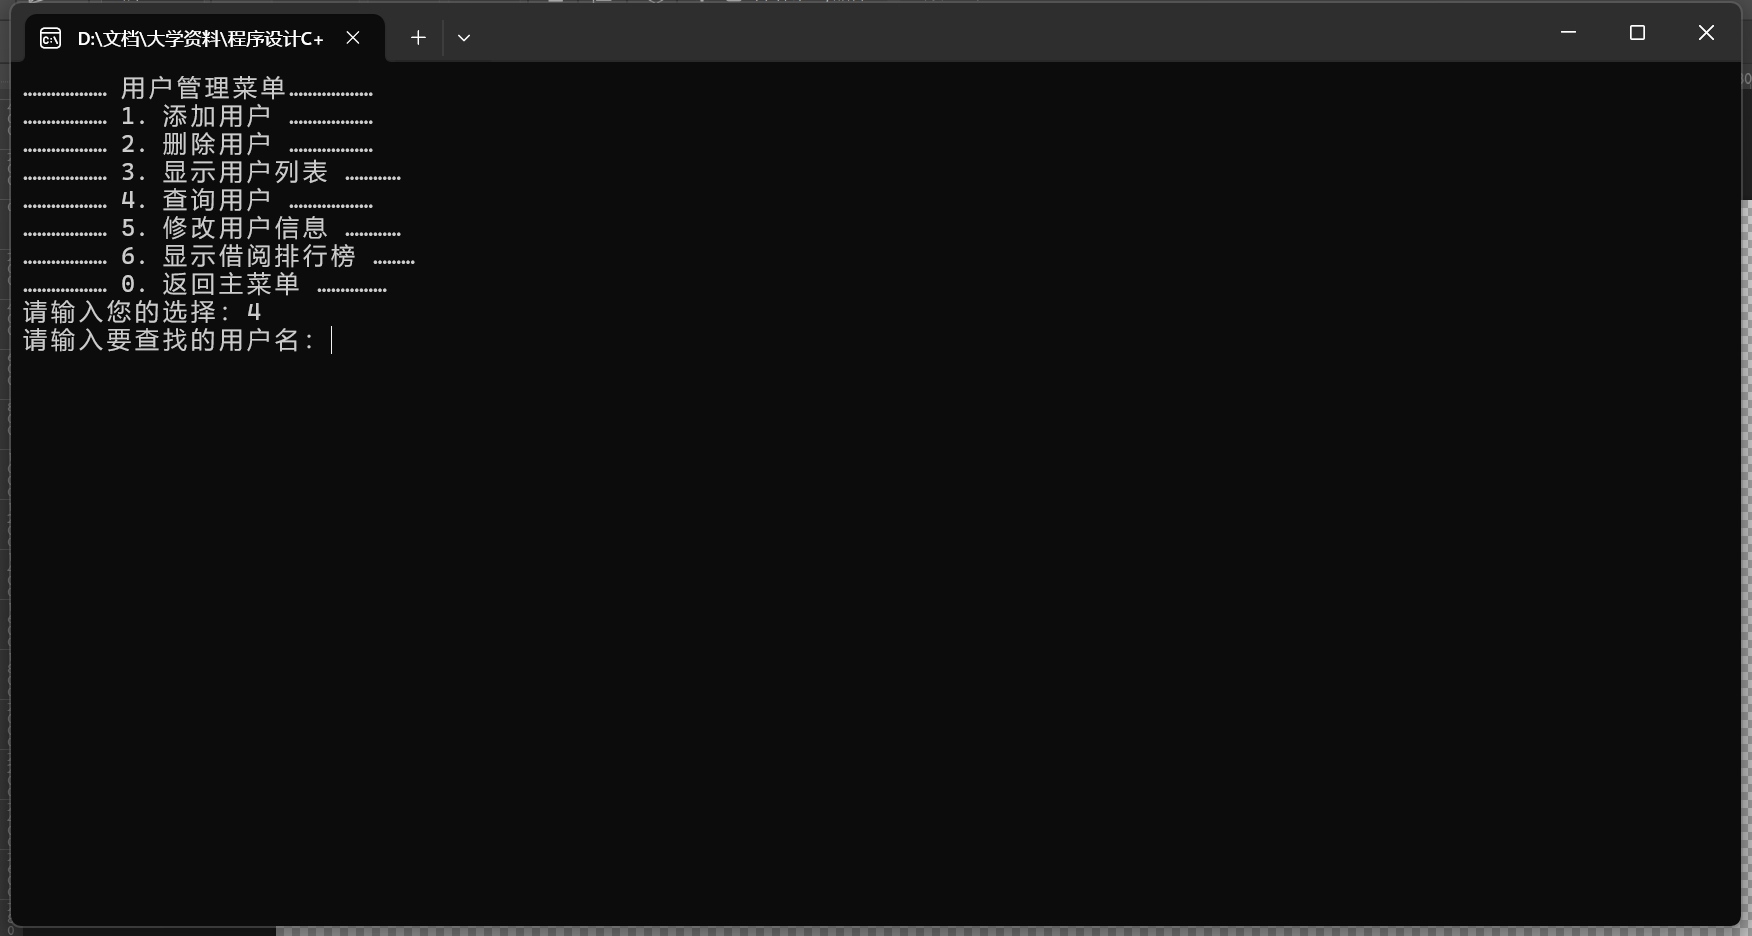
\includegraphics[width=0.8\textwidth]{searchuser.png}
    \caption{查找用户}
    \label{fig:searchuser}
\end{figure}

\begin{figure}[H]
    \centering
    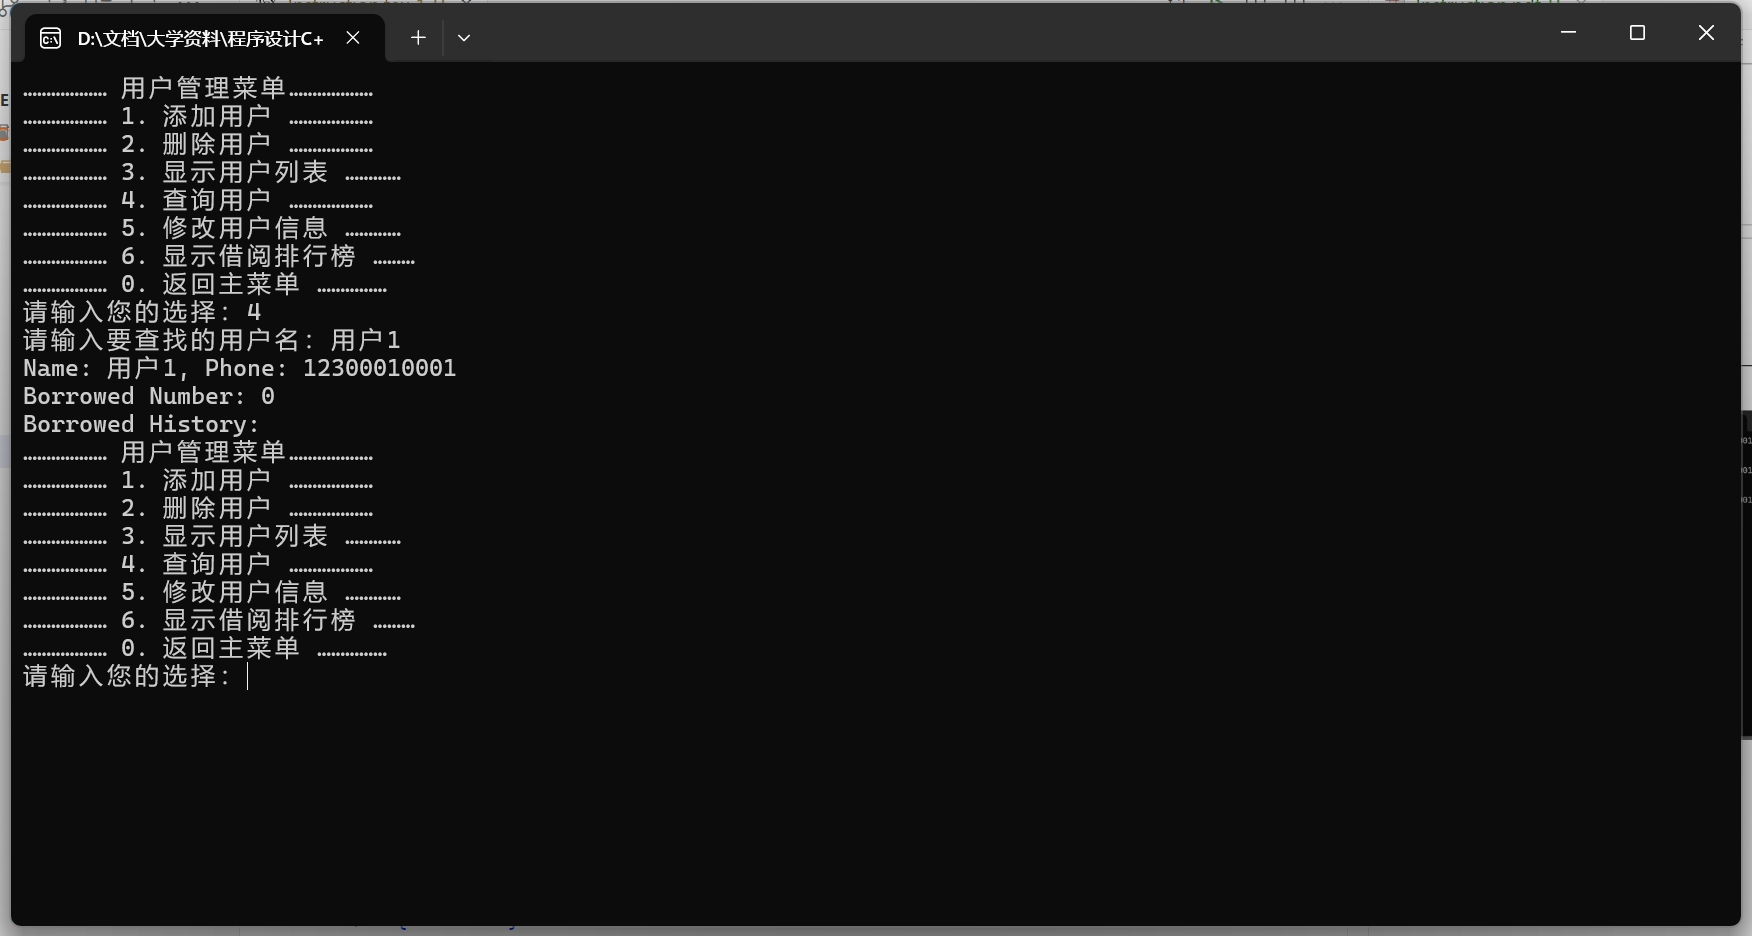
\includegraphics[width=0.8\textwidth]{searchresult.png}
    \caption{返回用户管理界面}
    \label{fig:searchresult}
\end{figure}

\subsubsection{修改用户信息}

\begin{figure}[H]
    \centering
    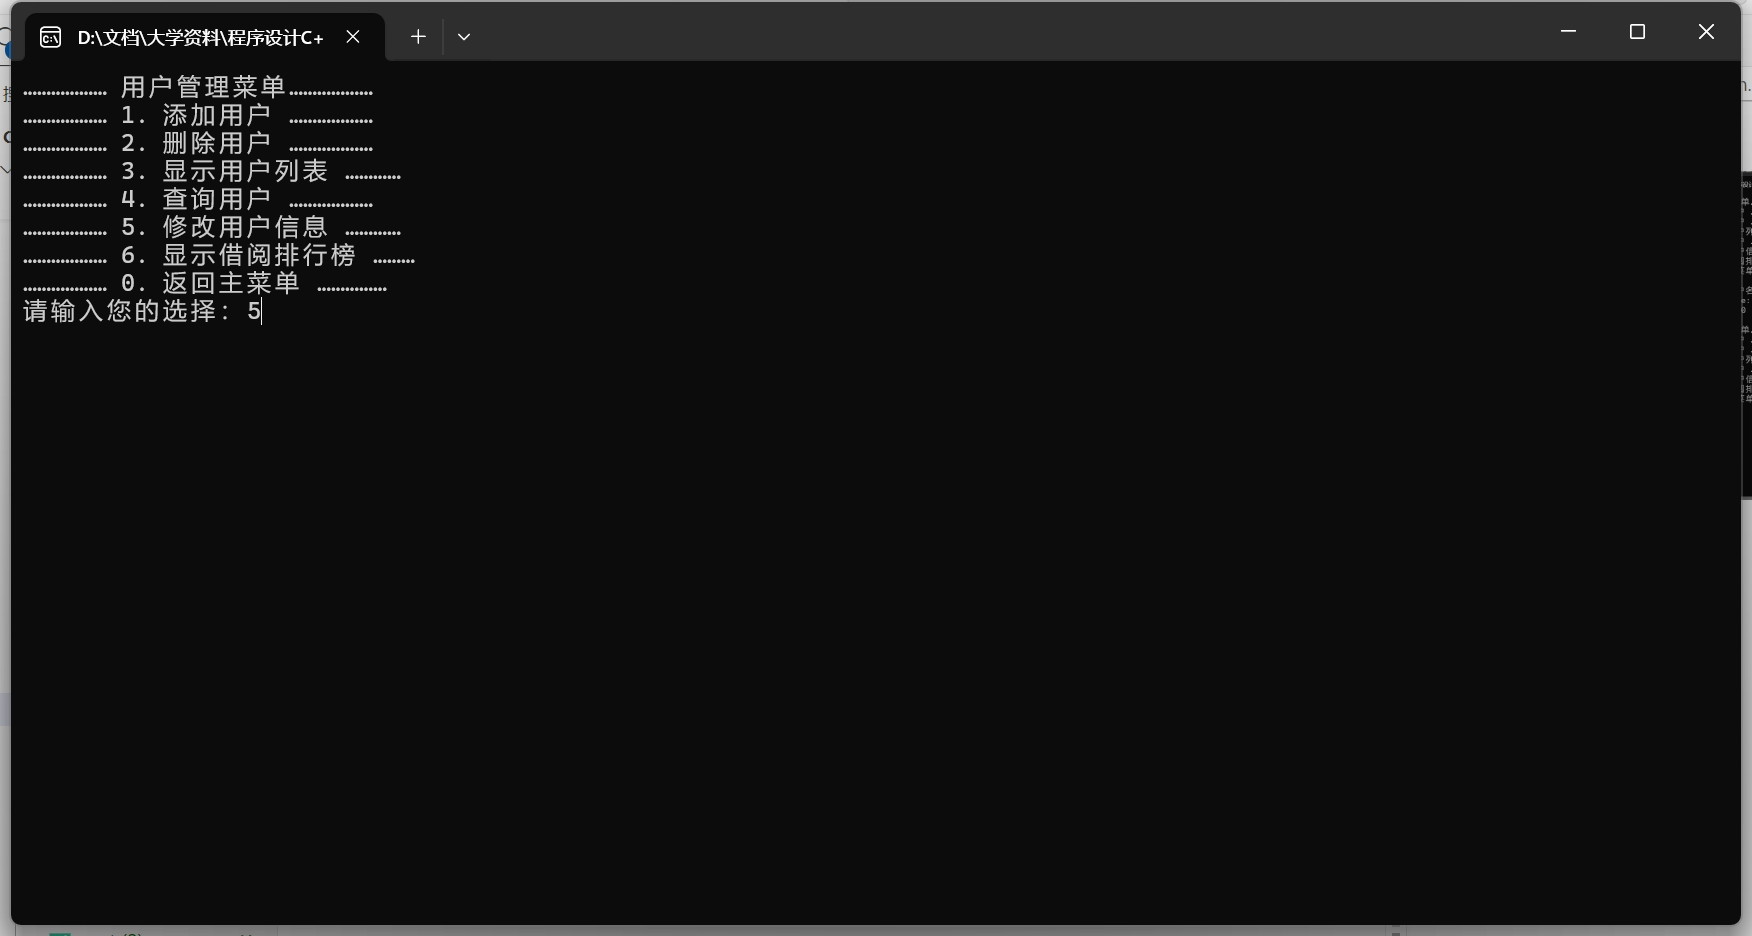
\includegraphics[width=0.8\textwidth]{selectchangeuser.png}
    \caption{选择修改用户信息}
\end{figure}

按照如图\ref{fig:changeuser}提示输入新的用户名和联系方式,系统会提示修改成功,
修改后的用户信息如图\ref{fig:changesuccess}所示。
\begin{figure}[H]
    \centering
    \begin{minipage}{0.48\textwidth}
        \centering
        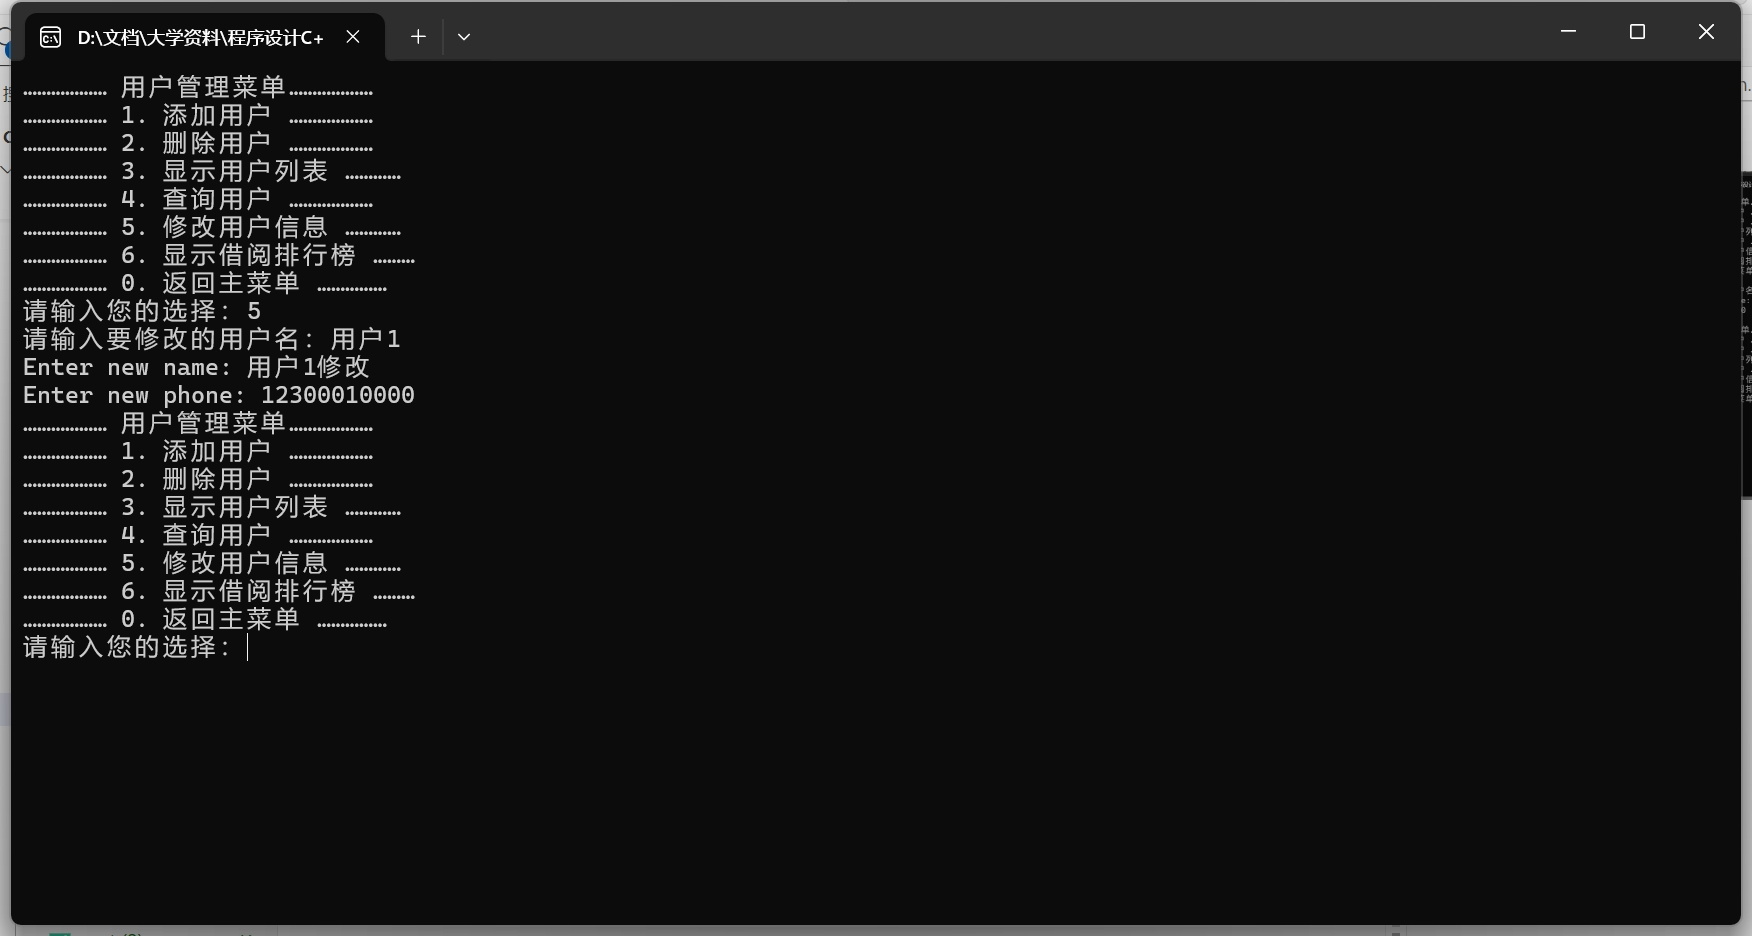
\includegraphics[width=\linewidth]{changeuser.png}
        \caption{修改用户信息}
        \label{fig:changeuser}
    \end{minipage}
    \hfill
    \begin{minipage}{0.48\textwidth}
        \centering
        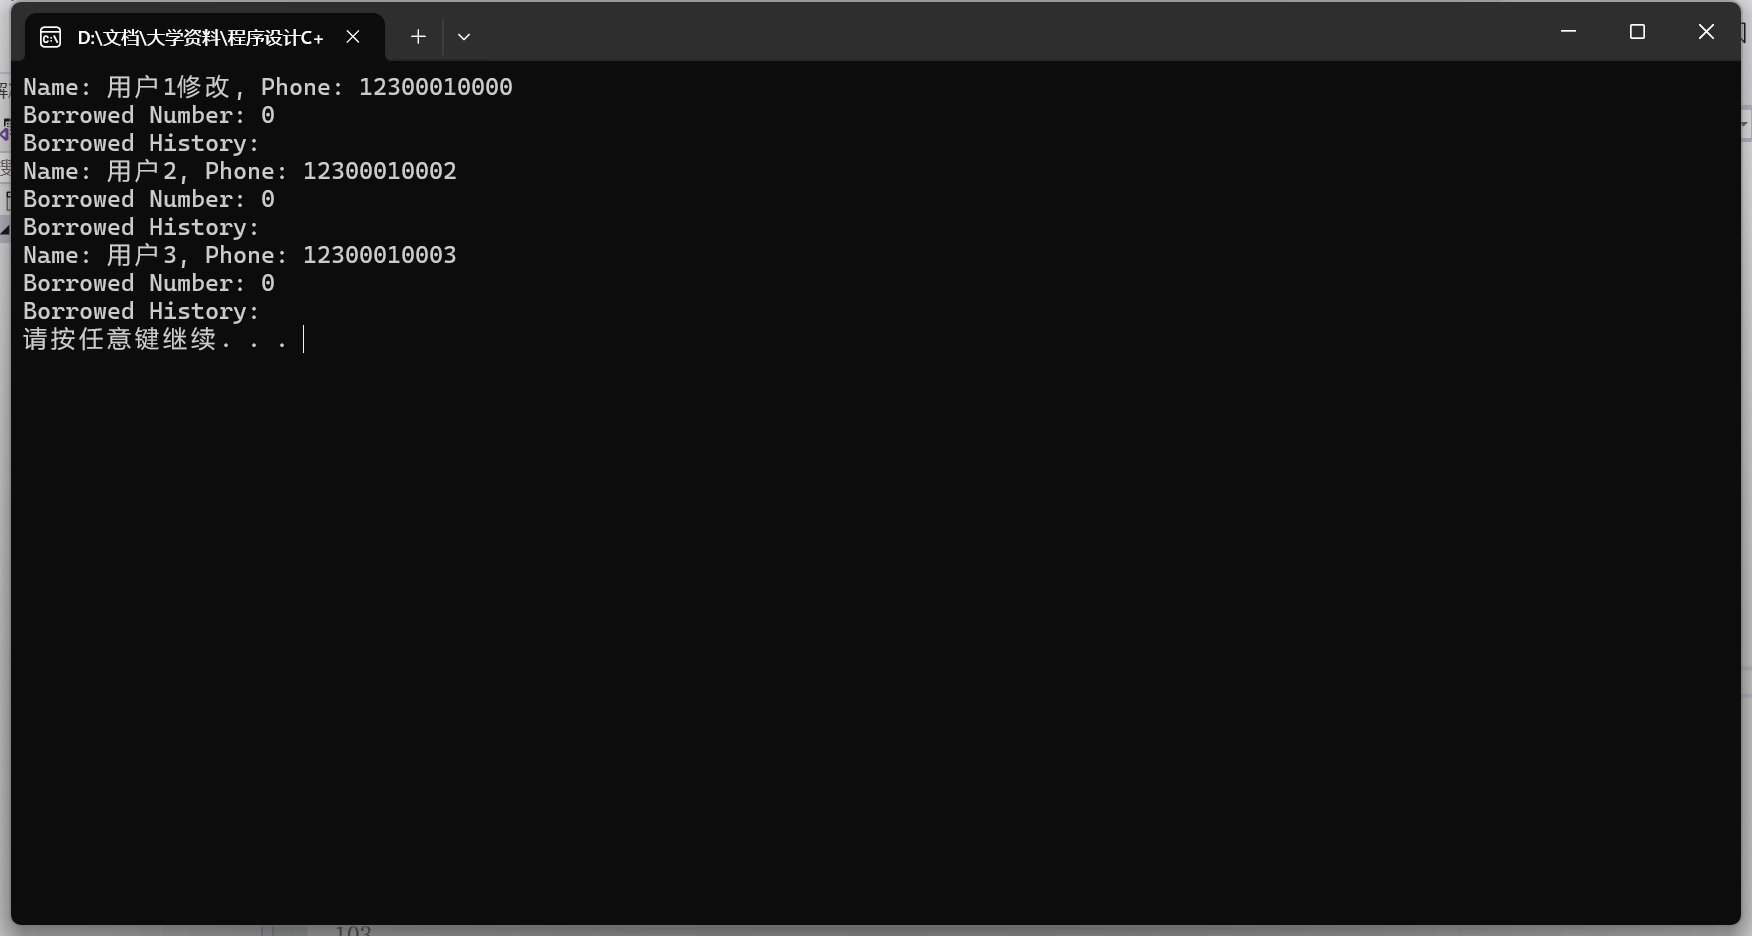
\includegraphics[width=\linewidth]{changed.png}
        \caption{修改之后的信息}
        \label{fig:changesuccess}
    \end{minipage}
\end{figure}

\subsubsection{借阅量排行榜}

\begin{figure}[H]
    \centering
    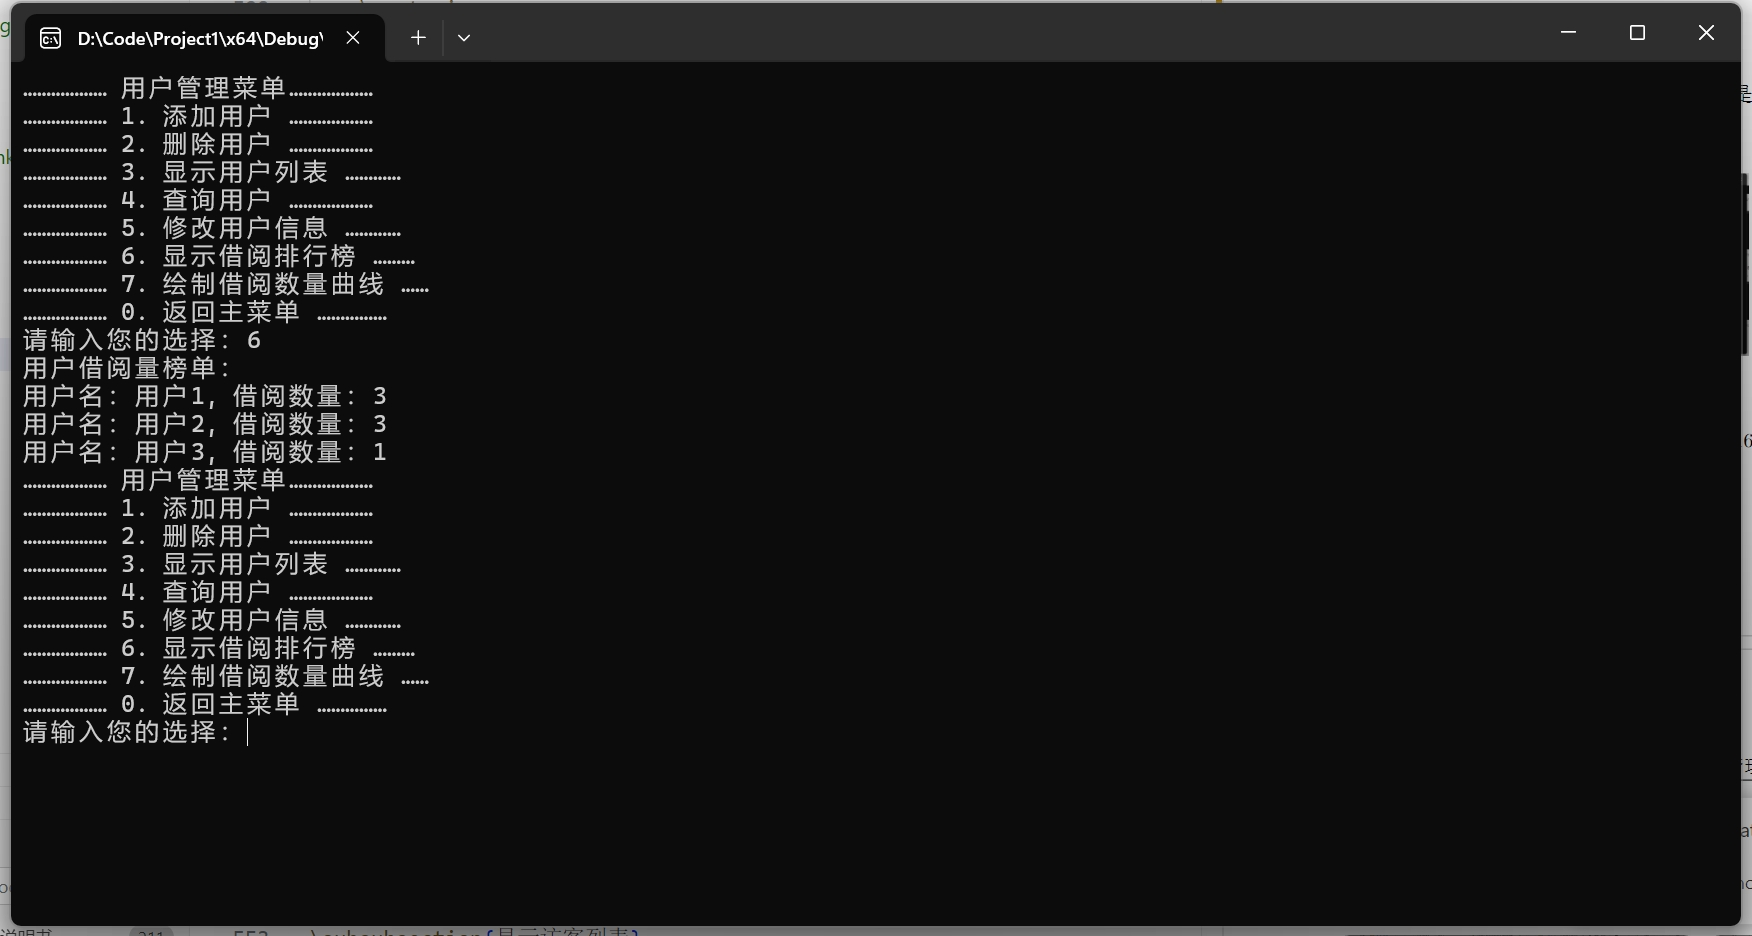
\includegraphics[width=0.8\textwidth]{UserRank.png}
    \caption{选择借阅量排行榜}
\end{figure}

\subsubsection{绘制借阅数量曲线}

在1.2.0版本中,新增了绘制借阅数量曲线的功能,用户可以选择绘制借阅数量曲线,
系统会自动绘制出借阅数量曲线,如图\ref{fig:UserCurve}所示。
左侧图显示了用户的借阅数量以及平均借阅量,右侧图显示了用户的借阅詹总借阅量比例。

\begin{figure}[H]
    \centering
    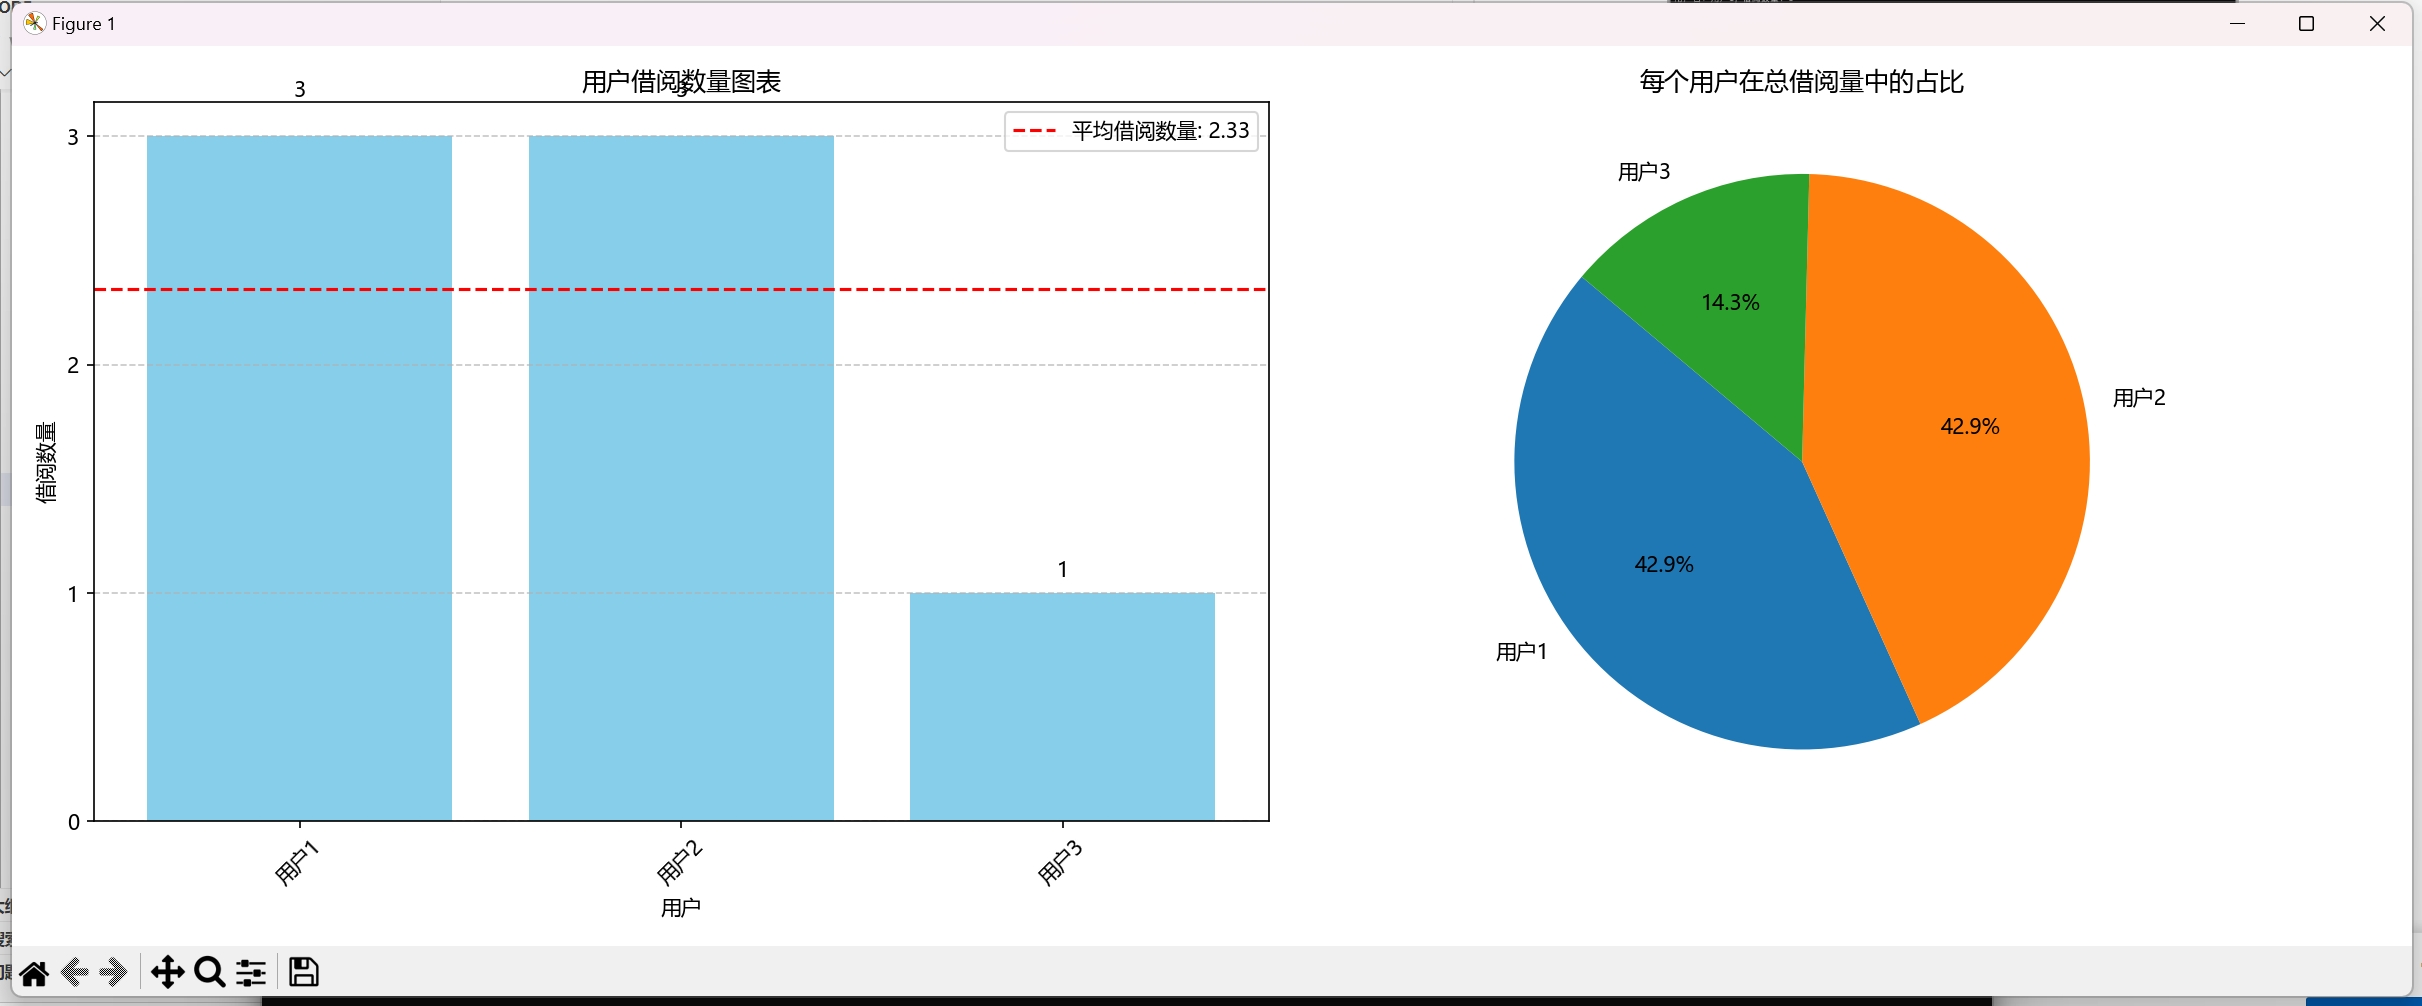
\includegraphics[width=0.8\textwidth]{UserCurve.png}
    \caption{借阅数量曲线}
    \label{fig:UserCurve}
\end{figure}

\newpage
\subsection{访客管理}

由于当前版本的访客管理功能较为简便没有实现复杂的访客模块,
因此在此不再赘述,只列出访客管理的功能列表,具体的操作流程与用户管理类似。

\subsubsection{添加访客}

\subsubsection{删除访客}

\subsubsection{显示访客列表}

\subsubsection{查找访客}

\subsubsection{修改访客信息}

\newpage
\subsection{管理员管理}

由于当前版本的管理员管理功能较为简单,尚未实现复杂的管理功能,
因此在此不再赘述,只列出管理员管理的功能列表,具体的操作流程与用户管理类似。

\subsubsection{添加管理员}

\subsubsection{删除管理员}

\subsubsection{显示管理员列表}

\subsubsection{查找管理员}

\subsubsection{修改管理员信息}

\newpage
\subsection{图书管理}

\begin{figure}[H]
    \centering
    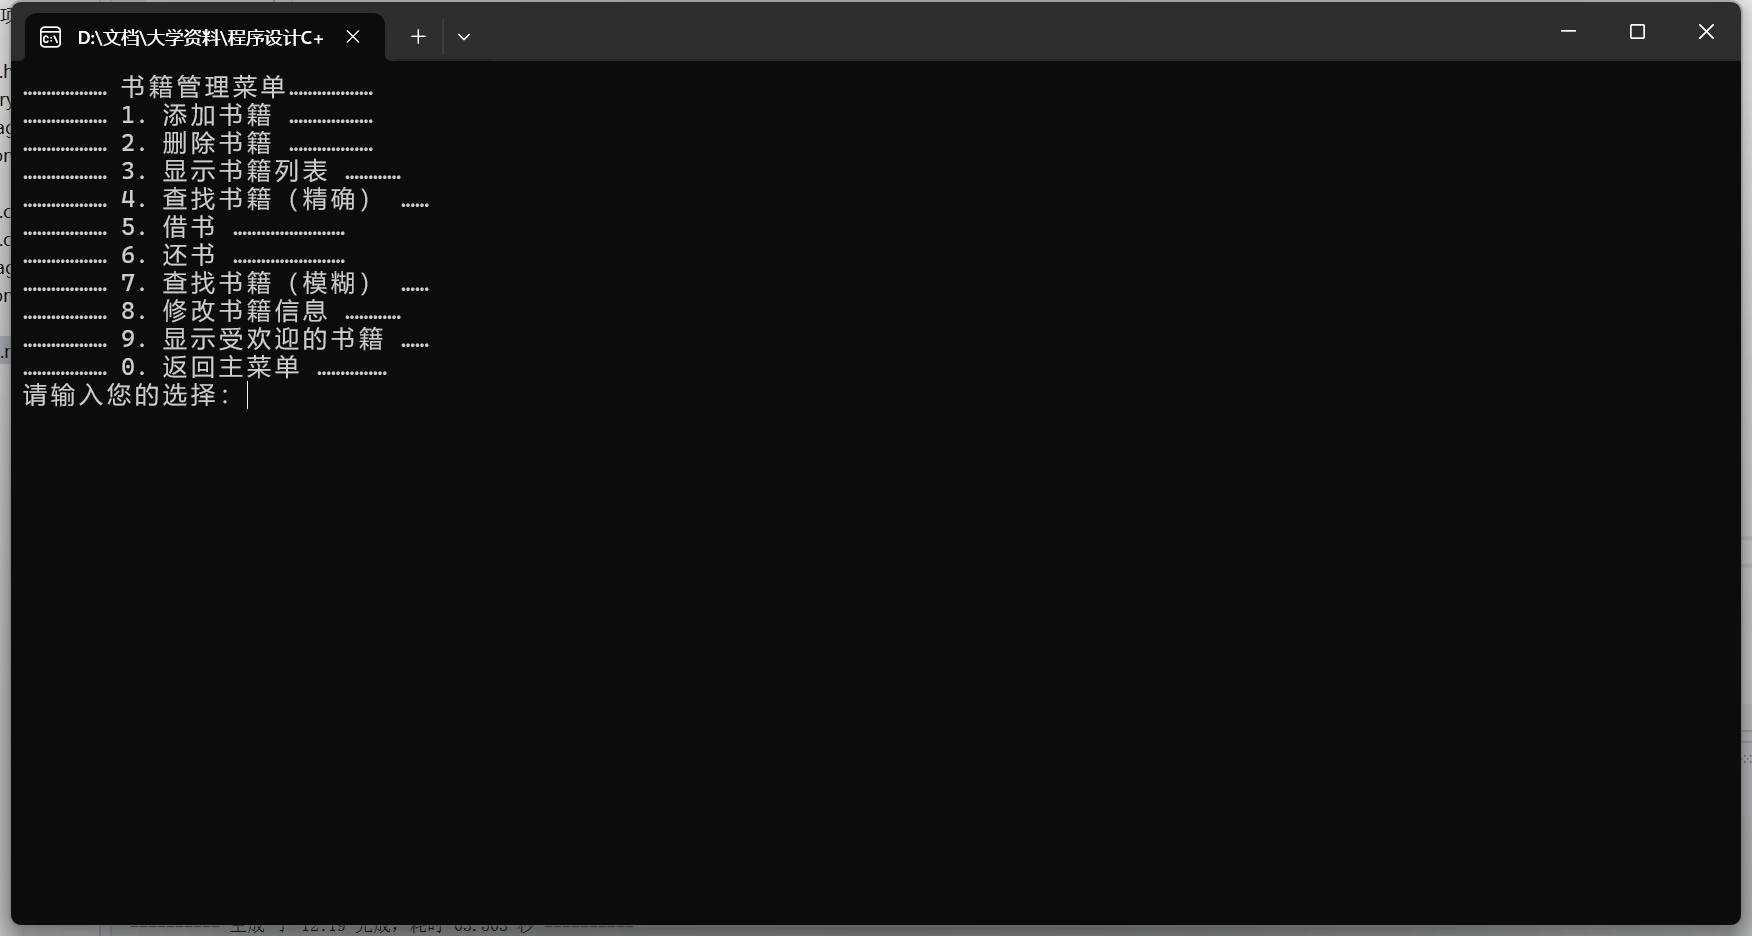
\includegraphics[width=0.8\textwidth]{Book/Bookmenu.png}
    \caption{进入图书管理界面}
\end{figure}

\subsubsection{添加图书}

\begin{figure}[H]
    \centering
    \begin{minipage}{0.48\textwidth}
        \centering
        \includegraphics[width=\linewidth]{Book/AddBookSucc.png}
        \caption{添加图书}
    \end{minipage}
    \hfill
    \begin{minipage}{0.48\textwidth}
        \centering
        \includegraphics[width=\linewidth]{Book/AddBook.png}
        \caption{添加图书成功}
    \end{minipage}
\end{figure}

$\ast $ \textit{目前尚不支持书名重复检测,只能检测出所有信息完全一致的书籍并给出提示,
    如果用户输入的图书已经存在,系统并不会提示用户,而是正常添加,
    并且在数据中会出现两本相同书名的图书。这个问题预计会在后续版本中解决。}


\subsubsection{删除图书}

\begin{figure}[H]
    \centering
    \includegraphics[width=0.8\textwidth]{Book/DeleteBookMenu.png}
    \caption{删除图书}
    \label{fig:DeleteBook}
\end{figure}

为确保不会由于误操作造成图书意外删除,删除图书要求输入准确地ISBN号码进行匹配,
如图\ref{fig:DeleteBook}所示,如果输入正确,系统会提示确认删除,如图\ref{fig:DeleteConfirm}所示,
如果确认删除,系统会提示删除成功,如图\ref{fig:Confirmed}所示。

同时为了便于查看书籍的具体信息,在选择显示书籍列表后,在进行删除操作时,并不会
进行清屏操作。

\begin{figure}[H]
    \centering
    \begin{minipage}{0.48\textwidth}
        \centering
        \includegraphics[width=\linewidth]{Book/DeleteConfirm.png}
        \caption{确认删除}
        \label{fig:DeleteConfirm}
    \end{minipage}
    \hfill
    \begin{minipage}{0.48\textwidth}
        \centering
        \includegraphics[width=\linewidth]{Book/Confirmed.png}
        \caption{删除图书成功}
        \label{fig:Confirmed}
    \end{minipage}
\end{figure}



\begin{figure}[H]
    \begin{minipage}[c]{0.45\textwidth}
        $\star$ 如果用户输入的ISBN号码有误,系统会提示删除失败,如图\ref{fig:DeleteFail}所示,
        用户可以重新输入正确的ISBN号码,然后再次尝试删除。
    \end{minipage}
    \hfill
    \begin{minipage}[c]{0.5\textwidth}
        \centering
        \includegraphics[width=\textwidth]{Book/DeleteBookFail.png}
        \caption{删除失败}
        \label{fig:DeleteFail}
    \end{minipage}
\end{figure}

\subsubsection{显示图书列表}

当用户选择显示图书列表时,系统会显示所有图书的信息,如图\ref{fig:Show}所示。

\begin{figure}[H]
    \centering
    \includegraphics[width=0.4\textwidth]{Book/Show.png}
    \caption{显示图书列表}
    \label{fig:Show}
\end{figure}

\subsubsection{查找图书}

\paragraph{精确查找}\mbox{}\\

本系统的精确查找目前仅支持ISBN号码的精确查找,用户输入ISBN号码后,
系统会返回该ISBN号码对应的图书信息,如图\ref{fig:Search1}所示。
如果输入的ISBN号码不存在或者输入有误,系统会提示用户输入有误,
如图\ref{fig:Search11}所示,用户可以检查ISBN号码是否输入正确,
然后重新输入。

\begin{figure}[H]
    \centering
    \begin{minipage}[c]{0.48\textwidth}
        \centering
        \includegraphics[width=\linewidth]{Book/Search1.png}
        \caption{ISBN精确查找}
        \label{fig:Search1}
    \end{minipage}
    \hfill
    \begin{minipage}[c]{0.48\textwidth}
        \centering
        \includegraphics[width=\linewidth]{Book/Search11.png}
        \caption{ISBN不存在或者输入有误}
        \label{fig:Search11}
    \end{minipage}
\end{figure}

\paragraph{模糊查找}\mbox{}\\

本系统的模糊查找支持两种方式:书名模糊查找和关键词模糊查找。
书名模糊查找是指用户输入书名的一部分,系统会返回所有书名中包含该部分的书籍。
如图\ref{fig:Search21}所示。
关键词模糊查找是指用户输入关键词中的一个,系统会返回所有关键字中包含该关键词的书籍。
如图\ref{fig:Search22}所示。

\begin{figure}[H]
    \centering
    \begin{minipage}{0.48\textwidth}
        \centering
        \includegraphics[width=\linewidth]{Book/Search2.png}
        \caption{书名模糊查找}
        \label{fig:Search21}
    \end{minipage}
    \hfill
    \begin{minipage}{0.48\textwidth}
        \centering
        \includegraphics[width=\linewidth]{Book/Search22.png}
        \caption{关键字模糊查找}
        \label{fig:Search22}
    \end{minipage}
\end{figure}


\subsubsection{修改图书信息}

如果需要修改图书信息,用户需要输入要修改的图书的名称,
如果图书存在,系统会返回该图书的信息,用户可以修改图书的全部信息,
如图\ref{fig:ModifyBook}所示,如果修改成功,书籍列表中的信息会进行更新,
如图\ref{fig:ModifySucc}所示。


\begin{figure}[H]
    \centering
    \begin{minipage}{0.48\textwidth}
        \centering
        \includegraphics[width=0.8\linewidth]{Book/modifybook.png}
        \caption{修改图书信息}
        \label{fig:ModifyBook}
    \end{minipage}
    \hfill
    \begin{minipage}{0.48\textwidth}
        \centering
        \includegraphics[width=0.8\linewidth]{Book/11modifybook.png}
        \caption{修改图书信息成功}
        \label{fig:ModifySucc}
    \end{minipage}
\end{figure}

$\star$ 特别提醒:在修改图书时,图书的信息为覆盖式修改,
即用户输入的信息会完全覆盖原有的信息,并且在修改时,关键词的
输入为逐个输入并确认,不需要用逗号分隔。

\subsubsection{借阅图书}

借阅书籍时,用户需要输入书名以及借阅用户名,
如果借阅成功,系统会提示借阅成功,如图\ref{fig:Borrow}所示,
同时书籍的节约状态和信息会同步更新,如图\ref{fig:ModifySucc}所示。
如果输入的书籍不存在或者输入有误,系统会提示用户输入有误,
如图\ref{fig:BorrowFail1}所示,用户可以检查书名是否输入正确,
然后重新输入。如果用户不存在,系统会提示用户不存在,
如图\ref{fig:BorrowFail2}所示,用户可以检查用户名是否输入正确,
然后重新输入。


\begin{figure}[H]
    \centering
    \includegraphics[width=0.6\textwidth]{Book/borrowsucc.png}
    \caption{借阅图书}
    \label{fig:Borrow}
\end{figure}

\begin{figure}[H]
    \centering
    \includegraphics[width=0.6\textwidth]{Book/borrowinginfo.png}
    \caption{借阅成功}
    \label{fig:ModifySuccess}
\end{figure}


\begin{figure}[H]
    \centering
    \begin{minipage}{0.48\textwidth}
        \centering
        \includegraphics[width=\textwidth]{Book/borrowsearchfail.png}
        \caption{书籍不存在或者输入有误}
        \label{fig:BorrowFail1}
    \end{minipage}\hfill
    \begin{minipage}{0.48\textwidth}
        \centering
        \includegraphics[width=\textwidth]{Book/borrowsearchuserfail.png}
        \caption{用户不存在}
        \label{fig:BorrowFail2}
    \end{minipage}
\end{figure}

\newpage
\subsubsection{归还图书}

归还书籍时,用户需要输入书名以及归还者的用户名,
如果归还成功,系统会提示归还成功,如图\ref{fig:Return}所示。出现这种情况可能是因为数据文件不存在或者数据文件损坏,用户可以检查数据文件是否存在或者尝试重新读取数据。

\begin{figure}[H]
    \centering
    \includegraphics[width=0.8\textwidth]{Book/returnsucc.png}
    \caption{归还图书}
    \label{fig:Return}
\end{figure}

$\star$ 特别提醒:当前系统仅支持逐本归还,并且在归还过程中\textbf{不会}对
借阅用户和归还用户的同一性进行检查:只要书籍已借出并且归还的用户存在,
就可以进行归还,并且借阅记录也正常。用户需要自行保证借阅用户和归还用户的一致性,
这个问题\textbf{可能}会在后续版本中解决,但是考虑到在实际使用过程中,
无论是哪一个用户进行归还,只要书籍能够正常归还,并不会造成书籍的损失,
并且这样的设计可以方便用户在无法到场的情况下进行归还,所以这个问题的
解决优先级较低。如果对此功能有更高的要求,可以与作者反馈,
作者会酌情在后续版本中进行修改。

\newpage
\subsubsection{显示借阅排行}

显示书籍的借阅量排行,系统会按照借阅量从高到低的顺序显示书籍的名称,
如图\ref{fig:BorrowList}所示。

\begin{figure}[H]
    \centering
    \includegraphics[width=0.8\textwidth]{Book/borrowlistq.png}
    \caption{显示借阅排行}
\end{figure}

\begin{figure}[H]
    \centering
    \includegraphics[width=0.8\textwidth]{Book/borrowlist.png}
    \caption{显示借阅排行}
    \label{fig:BorrowList}
\end{figure}

\newpage
\section{系统架构}

\subsection{类关系}
\begin{figure}[H]
    \centering
    \includegraphics[width=0.8\textwidth]{Pic/LibraryManagement.png}
    \caption{类关系图}
\end{figure}

\subsection{类的实现}

\subsubsection{基础类与人员类}
\begin{figure}[H]
    \centering
    \begin{minipage}{0.45\textwidth}
        \centering
        \includegraphics[width=\textwidth]{Pic/LibraryManagement/LibraryItem.png}
        \caption{LibraryItem}
    \end{minipage}\hfill
    \begin{minipage}{0.45\textwidth}
        \centering
        \includegraphics[width=\textwidth]{Pic/LibraryManagement/Person.png}
        \caption{Person}
    \end{minipage}
\end{figure}

\subsubsection{用户类与访客类}
\begin{figure}[H]
    \centering
    \begin{minipage}{0.45\textwidth}
        \centering
        \includegraphics[width=\textwidth]{Pic/LibraryManagement/User.png}
        \caption{User}
    \end{minipage}\hfill
    \begin{minipage}{0.45\textwidth}
        \centering
        \includegraphics[width=\textwidth]{Pic/LibraryManagement/Visitor.png}
        \caption{Visitor}
    \end{minipage}
\end{figure}

\subsubsection{管理员类与图书类}
\begin{figure}[H]
    \centering
    \begin{minipage}{0.45\textwidth}
        \centering
        \includegraphics[width=\textwidth]{Pic/LibraryManagement/Admin.png}
        \caption{Admin}
    \end{minipage}\hfill
    \begin{minipage}{0.45\textwidth}
        \centering
        \includegraphics[width=\textwidth]{Pic/LibraryManagement/Book.png}
        \caption{Book}
    \end{minipage}
\end{figure}

\subsubsection{图书管理类}
\begin{figure}[H]
    \centering
    \includegraphics[width=0.45\textwidth]{Pic/LibraryManagement/Management.png}
    \caption{Management}
\end{figure}

\newpage
\section{系统调试}

\subsection{调试环境}

% 调试环境的详细信息,使用表格格式进行更清晰的布局
% 增加行间距和列间距
\renewcommand{\arraystretch}{1.5}
\setlength{\tabcolsep}{10pt}
\begin{table}[h]
    \centering
    \begin{tabular}{>{\centering\arraybackslash}p{5cm}>{\centering\arraybackslash}p{10cm}}
        \hline
        \textbf{项目} & \textbf{描述}                                    \\ \hline
        操作系统        & Windows 11 家庭中文版                               \\
        版本号         & 22H2                                           \\
        操作系统版本      & 22621.3737                                     \\
        处理器         & 13th Gen Intel(R) Core(TM) i9-13900HX 2.20 GHz \\
        机带 RAM      & 16.0 GB (13.7 GB 可用)                           \\
        系统类型        & 64 位操作系统, 基于 x64 的处理器                          \\ \hline
    \end{tabular}
    \caption{系统信息}
\end{table}

\subsection{调试过程}

由于系统十分庞大,代码数量较多,为了能够准确判断错误的位置,
我采用逐步调试。整体上先搭建出框架,之后对每一部分的功能进行完善,
每实现一个功能,就进行一次调试,确保功能的正确性。在调试过程中,
我主要采用了输出调试的方法,通过输出一些关键的变量,来判断程序的运行情况,
并根据输出的结果来判断程序的正确性,所以源代码中存在的一些被注释掉的语句,
可能是用于调试时输出信息或者在调试时发现缺陷进行更改而遗留。
\par
在调试过程中,也出现了一些问题,比如在最初的设计中,并没有进行屏幕清理,
导致在输出信息时,屏幕上会出现大量的信息,不利于用户查看,为了解决这个问题,
我在适当位置加入了
\lstinline[language=C++]{system("pause"); system("cls");}
来暂停程序运行,等待用户确认后进行清屏,这样用户就可以清晰地看到输出的信息。
同时,在实际测试的过程中,我发现了在编程时遗漏的部分问题,比如输入格式有误、
输入信息内含空格等特殊情况,对此我也进行了进一步的改善,加入了一些输入检测功能,
并且更换了新的读取方式,尽最大可能地避免由于需要输入的内容本身造成的读取错误。
但是即便是输入成功,在村出纳数据以及读取数据时又出现了问题:应该如何保存
分属于不同类型的信息?在书籍信息部分,由于书籍的关键字可能含有多个,而在录入书籍
时,书籍的借阅历史为空,应该如何解决由此引发的各种矛盾?关于借阅历史,目前的版本中
采取的措施为默认添加"图书馆购入",既不会造成不合情理,又能有效解决问题。关于数据的
保存以及读取,我选择在保存时在适当的位置添加不同关键字以及分隔符号,
在读取时根据关键字以及分隔符号进行有效分隔,保证信息的准确性,保存的数据样式可以
查看\ref{sec:datafiles}部分。
\par
即使在编写完成之后,我进行了尽可能细致的调试工作,但是由于个人能力以及所遇见的
情况有限,不能保证考虑到所有可能出现的情况,所以可能存在一些尚未发现的潜在问题,
如果在实际使用过程中出现了难以捉摸的迷惑情况,可以重试一次,如果问题依旧存在,
可以发送邮件至\href{mailto:hy-huang23@mails.tsinghua.edu.cn}{hy-huang23@mails.tsinghua.edu.cn}
进行反馈,我会尽快进行处理。

\newpage
\section{系统更新}

\begin{table}[h]
    \centering
    \renewcommand{\arraystretch}{1.5} % 调整行高
    \setlength{\tabcolsep}{10pt} % 调整列间距
    \begin{tabular}{|c|c|}
        \hline
        \textbf{版本号} & \textbf{更新内容}                                                                                                          \\ \hline
        1.1.0        & \begin{tabular}[c]{@{}c@{}}- 修复了若干已知问题。\\ - 增加了新的功能特性。\\ - 改进了用户界面。\end{tabular}                                       \\ \hline
        1.2.0        & \begin{tabular}[c]{@{}c@{}}- 修复了若干已知问题。 \\ - 增加了用户借阅量条形图显示功能。\\ - 增加了用户借阅量占总借阅量比例饼图显示功能。\\ - 创新性地尝试多语言协同。\end{tabular} \\ \hline
    \end{tabular}
    \caption{软件更新历史}
\end{table}


\newpage
\section{后记}

\subsection{总结及致谢}
这应该是截至目前我编写过的最大的一个项目,
也是第一次完整地、独立地、一次性地完成一个
如此大型的项目代码编写。

上学期是我第一次系统性地学习编程,由于之前并没有什么编程基础,
在上学期感觉十分痛苦,课上讲的东西完全没有听说过,几乎没有什么概念,
在上学期的两次上机考试中,我也十分绝望:平时作业没有时间限制,还可以求助
同学,上网查询,但是上机考试要求在有限的时间完成一个全新的任务,
我的确感觉束手无策。

在假期,我决定自己从网上学一些C++,至少能做到上课不会一头雾水。
于是我也在网上找了一些教程,看了一些视频,尽管了解十分有限,
但还是让我对于程序设计有了一点最基本的信心。开学之后,
由于上学期学习过一些基本的语法,外加上假期的一小部分自学,
我感觉这学期的课程不在像上学期那样让人绝望,反而让我产生了一些兴趣。
但是当我看见这次的任务要求之后,还是感觉没有什么头绪。
虽然这次的要求十分明确,也不再像平时的作业那样断断续续,每次更新一点,
而是一次性完成一个完整的项目,但是我还是感觉不知从何下手。

一开始我遇见的一大难题是如何设计类,由于要求必须设计一个抽象类,我也进行了许多设想:
我想过设计一个基类之后派生出各种图书类型,但是这样就会导致图书类型没有办法自定义,
并且如果后续需要设计更精细的图书管理功能,就会变得十分复杂。最终,我决定设计一个
图书管理的抽象类,由此派生出图书类,在图书类中重写基类的纯虚函数,这样既满足了要求,
又不会导致后续的设计变得十分复杂。接着的一个困难就是如何设计多继承的派生类,
由于多继承需要考虑成员的二义性,并且需要设计合理。最终我选择管理员类进行多继承,
这样管理员兼具用户的借阅属性,又具备访客的访问次数,并独有管理权限这一属性,
这样的设计看起来会合常理一些。但是到目前,访客类和管理员类的功能尚未十分完善,
仅仅实现了基本的额添加、删除、查询、修改等基本功能,而二者各自的独有属性还没有
得到充分的体现,在后续的版本中我可能会根据现实生活中的需求,对这两个类的功能
进行进一步的完善。关于运算符重载,目前我将其设计在判断添加的书籍是否完全一致
的部分,后续也许会根据需要,再设计新的重载。

当我编写出主体功能后,我开始着手设计报表功能,虽然看起来十分简单,但是在实际
编写时,囿于C++的限制,我没有很好的办法来实现数据的图形化显示,而如果仅仅
把数据罗列输出,又无法达到很好的显示效果。当我一筹莫展的时候,我想到了调用
其他程序来显示数据的方法,比如Matlab和Python,这两个软件都有很好的数据可视化
功能。但是由于我对这两个软件的了解不够深入,水平仅仅停留在单纯使用一个的阶段,
从未尝试过通过其他程序来调用这两个软件进行绘图,所以我最终选择了较为简便并且
易于上网查询的Python。在原来程序的基础上,我将数据进行传出,在Python中接收
传来的数据,并根据数据进行绘图。通过这样的方式,我成功地实现了数据的图形化显示,
并且根据实际所需,我也在图形中加入了平均借阅量等信息,同时同步绘制了饼图,
显示用户的借阅量占总借阅量的比例。这样的设计看起来更加直观,也更加美观。
但是毕竟这是第一次尝试这样操作,很多地方并不够熟悉,调用的代码也多源于
网上现有的程序进行修改,所以在实际操作中,可能会感觉非常不自然并且会
出现多个窗口同时存在的情况,对此我目前也没有很好的解决办法。

关于界面的设计,通过查阅我了解到C++并没有很好的图形化界面功能,
如果想要实现图形化界面,需要调用QT等更高级的库,这显然已经超出了
我目前的能力范围。也许在未来的学习中,我会学习到更多的关于图形化
界面的知识,也许在未来的某个版本中,系统的界面会发生翻天覆地的变化,
但是在目前,我只能通过控制台进行界面的设计,这样的设计看起来十分简陋,
但是在实际使用中,也能够满足基本的需求。


\begin{quotation}
    Interest is the best teacher. --- Albert Einstein
\end{quotation}

也许当我真正开始对编程产生兴趣,而不再是为了应付考试的时候,
我才会真正地学会编程,也许这就是编程的魅力。当我真正开始设计这个系统,
并想要让它完善的时候,不论查资料还是问同学,无论写代码、改代码、测数据
还是编写说明书,我都觉得不再那么枯燥,反而随着系统的不断完善以及说明书
的不断成型,我感觉自己的编程能力也在不断提高,这种感觉是十分美妙的。刚刚开始
对程序设计产生如此浓厚的兴趣,这门课程却已接近尾声,我不知道以后还会
不会像这样写一个大型程序并给出详细的分析说明,也不知以后是否会使用新的编程语言,
但我始终相信,C++的学习将会成为我未来学习编程的基础,或许在某一天,
我会再打开这个系统,再打开这个说明书,再次回忆起这段编程的经历。

最后,再次感谢老师的悉心指导,感谢助教的耐心解答,感谢同学的互相帮助,也再次感谢
那个遇见困难没有放弃的自己,相信未来的路会越走越宽广,越走越精彩!

\newpage
\subsection{联系方式}

电子邮件:
\begin{itemize}
    \item 清华邮箱:\href{mailto:hy-huang23@mails.tsinghua.edu.cn}{hy-huang23@mails.tsinghua.edu.cn}
    \item QQ邮箱:\href{mailto:2253940186@qq.com}{2253940186@qq.com}
    \item Gmail邮箱:\href{mailto:haoyu6huang@gmail.com}{haoyu6huang@gmail.com}
\end{itemize}

\newpage
\subsection{版权声明}

\textit{本文档中的信息(包括 URL 及其他 Internet 网站参考资料)可能随时变更,
    恕不另行通知。使用本文档的全部风险或因此导致的后果均由用户自行承担。
    除非另外注明,否则此处作为例子提到的公司、组织、产品、域名、电子邮件地址、
    徽标、人员、地点和时间纯属虚构,绝不意指,也不应由此臆测任何真实的公司、组织、
    产品、域名、电子邮件地址、徽标、人员、地点和时间。}

\textbf{版权所有 © 2024 黄皓宇。保留所有权利。}

本文档是由 黄皓宇 提供的,仅供参考之用。未经 黄皓宇 事先书面同意,
不得以任何形式或手段(电子、机械、影印或其他方式)复制、分发、修改、重用、
再发布或利用本文档的任何部分进行商业利用。


\newpage
\section{附录}

\subsection{源代码}
由于用户指南制作时的格式问题,以下源代码中的\textbf{中文全部替换成了英文},
但是实现的功能和效果与中文版本\underline{\textbf{完全一致}},如果需要查看中文版本的源代码,
请点击\href{https://github.com/Alex-hwang/BookManagementSystem}{\underline{源代码}}查看。

\par
本系统的所有代码文件以及数据文件均已上传至清华云盘。
请点击\href{https://cloud.tsinghua.edu.cn/d/ce27972bcd2b428abddb/}{\underline{这里}}下载源代码文件。

\newpage
\subsubsection{LibraryItem.h}

\begin{lstlisting}[language=C++]
#ifndef LIBRARYITEM_H
#define LIBRARYITEM_H

#pragma warning(disable : 4996)
#define _CRT_SECURE_NO_WARNINGS

#include <string>

class LibraryItem {
public:
    virtual ~LibraryItem() = default;

    virtual std::string getTitle() = 0;
    virtual void setTitle(std::string title) = 0;
    virtual void showBookInfo() = 0;
};

#endif // LIBRARYITEM_H
\end{lstlisting}

\newpage
\subsubsection{Person.h}

\begin{lstlisting}[language=C++]
#ifndef PERSON_H
#define PERSON_H

#pragma warning(disable : 4996)
#define _CRT_SECURE_NO_WARNINGS

#include <vector>
#include <string>

class Person {
protected:
    std::string m_name;
    std::string m_phone;

public:
    Person();
    Person(std::string name, std::string phone);

    virtual ~Person() = 0;

    std::string getName() const;
    std::string getPhone() const;
    void setName(std::string name);
    void setPhone(std::string phone);

    virtual void showPersonInfo() const;
    virtual void modifyPersonInfo();
};

class User : virtual public Person {
private:
    int m_borrowingNum;
    int m_borrowedNum;
    std::vector<std::string> m_borrowedHistory;

public:
    User();
    User(std::string name, std::string phone);
    User(std::string name, std::string phone, int borrowingNum, std::vector<std::string> borrowedHistory);

    ~User() override;

    int getborrowingNum() const;
    int getBorrowedNum() const;
    std::vector<std::string> getBorrowedHistory() const;
    void setborrowingNum(int borrowingNum);
    void setBorrowedHistory(std::vector<std::string> borrowedHistory);

    void showUserInfo() const;
    void borrowBook(std::string bookName);
    void returnBook(std::string bookName);
    void showBorrowHistory() const;
};

class Visitor : virtual public Person {
private:
    int m_visitNum;

public:
    Visitor();
    Visitor(std::string name, std::string phone);
    Visitor(std::string name, std::string phone, int visitNum);

    ~Visitor() override;

    int getVisitNum() const;
    void setVisitNum(int visitNum);

    void modifyVisitorInfo();
    void showVisitorInfo() const;
};

class Admin : public User, public Visitor {
private:
    int m_authority;

public:
    Admin();
    Admin(std::string name, std::string phone);
    Admin(std::string name, std::string phone, int borrowingNum, std::vector<std::string> borrowedHistory, int visitNum, int authority);

    ~Admin() override;

    int getAuthority() const;
    void setAuthority(int authority);

    void modifyAdminInfo();
    void showAdminInfo() const;
};

#endif // PERSON_H
\end{lstlisting}

\newpage
\subsubsection{Book.h}

\begin{lstlisting}[language=C++]
#ifndef BOOK_H
#define BOOK_H

#define _CRT_SECURE_NO_WARNINGS

#include <iostream>
#include <string>
#include <vector>
#include "LibraryItem.h"
#include "Person.h"
using namespace std;

// Book class
class Book : public LibraryItem
{
public:
    // Constructors
    Book();
    Book(const Book& book);
    Book(std::string name, std::string author, std::string type, vector<std::string> keywords, std::string introduction, std::string ISBN, double price);
    Book(std::string name, std::string author, std::string type, vector<std::string> keywords, std::string introduction, bool borrowed, vector<std::string> borrowHistory, int borrowTimes, std::string ISBN, double price);

    ~Book();

    // Getters and Setters
    std::string getTitle();
    std::string getAuthor();
    std::string getType();
    vector<std::string> getKeywords();
    std::string getIntroduction();
    bool getBorrowed();
    vector<std::string> getBorrowHistory();
    int getBorrowTimes();
    std::string getISBN();
    double getPrice();

    void setTitle(std::string name);
    void setAuthor(std::string author);
    void setType(std::string type);
    void setKeywords(vector<std::string> keywords);
    void setIntroduction(std::string introduction);
    void setBorrowed(bool borrowed);
    void setBorrowHistory(vector<std::string> borrowHistory);
    void setBorrowTimes(int borrowTimes);
    void setISBN(std::string ISBN);
    void setPrice(double price);

    // Display book information
    void showBookInfo();

    // Borrow a book
    void borrowBook(const User user);
    // Return a book
    void returnBook();

    // Check if the book is borrowed
    bool isBorrowed();

    // Fuzzy matching
    // Check if the book matches the keyword
    bool isMatchKeyword(std::string keyword);
    // Check if the book matches the author
    bool isMatchAuthor(std::string author);
    // Check if the book matches the type
    bool isMatchType(std::string type);
    // Check if the book matches the name
    bool isMatchName(std::string name);
    // Check if the book matches the introduction
    bool isMatchIntroduction(std::string introduction);
    // General fuzzy matching
    bool isMatch(std::string word);

    // Operator overloading
    bool operator==(const Book& rhs) const;

    // Exact search
    // Check if the book matches the ISBN
    bool isMatchISBN(std::string ISBN);

    // Modify book information
    void modifyBookInfo();

private:
    // Book attributes: name, author, type, keywords, introduction, borrow status, borrow history, borrow times, ISBN, price
    std::string m_name;
    std::string m_author;
    std::string m_type;
    vector<std::string> m_keywords;
    std::string m_introduction;
    bool m_borrowed;
    vector<std::string> m_borrowHistory;
    int m_borrowTimes;
    std::string m_ISBN;
    double m_price;
};

#endif // BOOK_H
\end{lstlisting}

\newpage
\subsubsection{Management.h}

\begin{lstlisting}[language=C++]
#ifndef MANAGEMENT_H // If MANAGEMENT_H is not defined
#define MANAGEMENT_H // Define MANAGEMENT_H

#include <vector>
#include "Person.h"
#include "Book.h"

class Management
{
public:
    Management();
    ~Management();

    // User management
    void addUser();
    void deleteUser();
    void showUserList() const;
    void searchUser() const;
    void modifyUserInfo();

    // Visitor management
    void addVisitor();
    void deleteVisitor();
    void showVisitorList() const;
    void searchVisitor() const;
    void modifyVisitorInfo();

    // Admin management
    void addAdmin();
    void deleteAdmin();
    void showAdminList() const;
    void searchAdmin() const;
    void modifyAdminInfo();

    // Book management
    void addBook();
    void deleteBook();
    void showBookList();
    void searchBookSpecifically();
    void borrowBook();
    void returnBook();
    void searchBook(std::vector<Book> m_bookList);
    void modifyBookInfo();

    // Report features
    void showMostPopularBooks(); // Display the list of most popular books
    void showTopBorrowers();     // Display the list of top borrowers
    void showChart();

    // Data management
    void saveData();
    void readData();

    // Main menu
    void start();
    void showMainMenu() const;

    // Submenus
    void userMenu();
    void visitorMenu();
    void adminMenu();
    void bookMenu();
    void dataMenu();

private:
    std::vector<User> m_userList;
    std::vector<Visitor> m_visitorList;
    std::vector<Admin> m_adminList;
    std::vector<Book> m_bookList;
};

#endif // MANAGEMENT_H // End of preprocessor directive
\end{lstlisting}

\newpage
\subsubsection{Person.cpp}

\begin{lstlisting}[language=C++]
#include "Person.h"
#include <iostream>

// Implementation of the Person class
Person::Person() : m_name("Unknown"), m_phone("Unknown") {}

Person::Person(std::string name, std::string phone) : m_name(name), m_phone(phone) {}

Person::~Person() {}

std::string Person::getName() const
{
    return m_name;
}

std::string Person::getPhone() const
{
    return m_phone;
}

void Person::setName(std::string name)
{
    m_name = name;
}

void Person::setPhone(std::string phone)
{
    m_phone = phone;
}

void Person::showPersonInfo() const
{
    std::cout << "Name: " << m_name << ", Phone: " << m_phone << std::endl;
}

void Person::modifyPersonInfo()
{
    std::cout << "Enter new name: ";
    std::cin >> m_name;
    std::cout << "Enter new phone: ";
    std::cin >> m_phone;
}

// Implementation of the User class
User::User() : Person(), m_borrowingNum(0) {}

User::User(std::string name, std::string phone) : Person(name, phone), m_borrowingNum(0) {}

User::User(std::string name, std::string phone, int borrowingNum, std::vector<std::string> borrowedHistory)
    : Person(name, phone), m_borrowingNum(borrowingNum), m_borrowedHistory(borrowedHistory) {}

User::~User() {}

int User::getborrowingNum() const
{
    return m_borrowingNum;
}

int User::getBorrowedNum() const
{
    return m_borrowedNum;
}

std::vector<std::string> User::getBorrowedHistory() const
{
    return m_borrowedHistory;
}

void User::setborrowingNum(int borrowingNum)
{
    m_borrowingNum = borrowingNum;
}

void User::setBorrowedHistory(std::vector<std::string> borrowedHistory)
{
    m_borrowedHistory = borrowedHistory;
}

void User::showUserInfo() const
{
    showPersonInfo();
    std::cout << "Borrowed Number: " << m_borrowingNum << std::endl;
    std::cout << "Borrowed History: ";
    for (const auto &book : m_borrowedHistory)
    {
        std::cout << book << " ";
    }
    std::cout << std::endl;
}

void User::borrowBook(std::string bookName)
{
    m_borrowingNum++;
    m_borrowedNum++;
    m_borrowedHistory.push_back(bookName);
}

void User::returnBook(std::string bookName)
{
    auto it = std::find(m_borrowedHistory.begin(), m_borrowedHistory.end(), bookName);
    if (it != m_borrowedHistory.end() && m_borrowingNum > 0)
    {
        // m_borrowingNum--;
        return;
    }
}

void User::showBorrowHistory() const
{
    std::cout << "Borrowed History: ";
    for (const auto &book : m_borrowedHistory)
    {
        std::cout << book << " ";
    }
    std::cout << std::endl;
}

// Implementation of the Visitor class
Visitor::Visitor() : Person(), m_visitNum(0) {}

Visitor::Visitor(std::string name, std::string phone) : Person(name, phone), m_visitNum(0) {}

Visitor::Visitor(std::string name, std::string phone, int visitNum) : Person(name, phone), m_visitNum(visitNum) {}

Visitor::~Visitor() {}

int Visitor::getVisitNum() const
{
    return m_visitNum;
}

void Visitor::setVisitNum(int visitNum)
{
    m_visitNum = visitNum;
}

void Visitor::modifyVisitorInfo()
{
    modifyPersonInfo();
    std::cout << "Enter new visit number: ";
    std::cin >> m_visitNum;
}

void Visitor::showVisitorInfo() const
{
    showPersonInfo();
    std::cout << "Visit Number: " << m_visitNum << std::endl;
}

// Implementation of the Admin class
Admin::Admin() : Person(), User(), Visitor(), m_authority(0) {}

Admin::Admin(std::string name, std::string phone)
    : Person(name, phone), User(name, phone), Visitor(name, phone), m_authority(0) {}

Admin::Admin(std::string name, std::string phone, int borrowingNum, std::vector<std::string> borrowedHistory, int visitNum, int authority)
    : Person(name, phone), User(name, phone, borrowingNum, borrowedHistory), Visitor(name, phone, visitNum), m_authority(authority) {}

Admin::~Admin() {}

int Admin::getAuthority() const
{
    return m_authority;
}

void Admin::setAuthority(int authority)
{
    m_authority = authority;
}

void Admin::modifyAdminInfo()
{
    modifyPersonInfo();
    std::cout << "Enter new authority level: ";
    std::cin >> m_authority;
}

void Admin::showAdminInfo() const
{
    showUserInfo();
    showVisitorInfo();
    std::cout << "Authority Level: " << m_authority << std::endl;
}
\end{lstlisting}

\newpage
\subsubsection{Book.cpp}

\begin{lstlisting}[language=C++]
#include "Book.h"

// Implementation of the Book class
Book::Book()
{
    m_name = "";
    m_author = "";
    m_type = "";
    m_keywords.clear();
    m_introduction = "";
    m_borrowed = false;
    m_borrowHistory = {};
    m_borrowTimes = 0;
    m_ISBN = "";
    m_price = 0;
}

Book::Book(std::string name, std::string author, std::string type, vector<std::string> keywords, std::string introduction, bool borrowed, vector<std::string> borrowHistory, int borrowTimes, std::string ISBN, double price)
{
    m_name = name;
    m_author = author;
    m_type = type;
    m_keywords = keywords;
    m_introduction = introduction;
    m_borrowed = borrowed;
    m_borrowHistory = borrowHistory;
    m_borrowTimes = borrowTimes;
    m_ISBN = ISBN;
    m_price = price;
}

Book::Book(const Book &book)
{
    m_name = book.m_name;
    m_author = book.m_author;
    m_type = book.m_type;
    m_keywords = book.m_keywords;
    m_introduction = book.m_introduction;
    m_borrowed = book.m_borrowed;
    m_borrowHistory = book.m_borrowHistory;
    m_borrowTimes = book.m_borrowTimes;
    m_ISBN = book.m_ISBN;
    m_price = book.m_price;
}

Book::Book(std::string title, std::string author, std::string type, std::vector<string> keywords, std::string introduction, std::string ISBN, double price)
{
    m_name = title;
    m_author = author;
    m_type = type;
    m_keywords = keywords;
    m_introduction = introduction;
    m_borrowed = false;
    m_borrowHistory = {};
    m_borrowTimes = 0;
    m_ISBN = ISBN;
    m_price = price;
}

Book::~Book()
{
    // cout << "Book object destroyed" << endl;
}

std::string Book::getTitle()
{
    return m_name;
}

std::string Book::getAuthor()
{
    return m_author;
}

std::string Book::getType()
{
    return m_type;
}

vector<std::string> Book::getKeywords()
{
    return m_keywords;
}

std::string Book::getIntroduction()
{
    return m_introduction;
}

bool Book::getBorrowed()
{
    return m_borrowed;
}

vector<std::string> Book::getBorrowHistory()
{
    return m_borrowHistory;
}

int Book::getBorrowTimes()
{
    return m_borrowTimes;
}

std::string Book::getISBN()
{
    return m_ISBN;
}

double Book::getPrice()
{
    return m_price;
}

void Book::setTitle(std::string name)
{
    m_name = name;
}

void Book::setAuthor(std::string author)
{
    m_author = author;
}

void Book::setType(std::string type)
{
    m_type = type;
}

void Book::setKeywords(vector<std::string> keywords)
{
    m_keywords = keywords;
}

void Book::setIntroduction(std::string introduction)
{
    m_introduction = introduction;
}

void Book::setBorrowed(bool borrowed)
{
    m_borrowed = borrowed;
}

void Book::setBorrowHistory(vector<std::string> borrowHistory)
{
    m_borrowHistory = borrowHistory;
}

void Book::setBorrowTimes(int borrowTimes)
{
    m_borrowTimes = borrowTimes;
}

void Book::setISBN(std::string ISBN)
{
    m_ISBN = ISBN;
}

void Book::setPrice(double price)
{
    m_price = price;
}

void Book::showBookInfo()
{
    cout << "Title: " << m_name << endl;
    cout << "Author: " << m_author << endl;
    cout << "Type: " << m_type << endl;
    cout << "Keywords: ";
    for (int i = 0; i < m_keywords.size(); i++)
    {
        cout << m_keywords[i] << " ";
    }
    cout << endl;
    cout << "Introduction: " << m_introduction << endl;
    cout << "Borrow status: " << (m_borrowed ? "Borrowed" : "Available") << endl;
    cout << "ISBN: " << m_ISBN << endl;
    cout << "Price: " << m_price << endl;
    cout << "Borrow history: ";
    for (int i = 0; i < m_borrowHistory.size(); i++)
    {
        cout << m_borrowHistory[i] << " ";
    }
    cout << endl;
}

void Book::borrowBook(User user)
{
    m_borrowed = true;
    time_t now = time(0);
    tm *ltm = localtime(&now);
    std::string borrowTime = to_string(1900 + ltm->tm_year) + "-" + to_string(1 + ltm->tm_mon) + "-" + to_string(ltm->tm_mday);
    m_borrowHistory.push_back(user.getName() + " " + borrowTime);
    m_borrowTimes++;
}

void Book::returnBook()
{
    m_borrowed = false;
    time_t now = time(0);
    tm *ltm = localtime(&now);
    std::string returnTime = to_string(1900 + ltm->tm_year) + "-" + to_string(1 + ltm->tm_mon) + "-" + to_string(ltm->tm_mday);
    m_borrowHistory.back() += " " + returnTime;
    m_borrowTimes++;
}

bool Book::isBorrowed()
{
    return m_borrowed;
}

bool Book::isMatchKeyword(std::string keyword)
{
    for (const auto &kw : m_keywords)
    {
        if (kw.find(keyword) != std::string::npos)
        {
            return true;
        }
    }
    return false;
}

bool Book::isMatchAuthor(std::string author)
{
    return m_author.find(author) != std::string::npos;
}

bool Book::isMatchType(std::string type)
{
    return m_type.find(type) != std::string::npos;
}

bool Book::isMatchName(std::string name)
{
    return m_name.find(name) != std::string::npos;
}

bool Book::isMatchIntroduction(std::string introduction)
{
    return m_introduction.find(introduction) != std::string::npos;
}

bool Book::isMatchISBN(std::string ISBN)
{
    return m_ISBN == ISBN;
}

bool Book::isMatch(std::string word)
{
    return isMatchKeyword(word) || isMatchAuthor(word) || isMatchType(word) || isMatchName(word) || isMatchIntroduction(word);
}

void Book::modifyBookInfo()
{
    cout << "Enter title: ";
    cin >> m_name;
    cout << "Enter author: ";
    cin >> m_author;
    cout << "Enter type: ";
    cin >> m_type;
    cout << "Enter keywords: ";
    m_keywords.clear();
    while (true)
    {
        std::string keyword;
        cin >> keyword;
        m_keywords.push_back(keyword);
        cout << "Continue entering keywords? (y/n)";
        char c;
        cin >> c;
        if (c == 'n')
        {
            break;
        }
    }
    cout << "Enter introduction: ";
    cin >> m_introduction;
    cout << "Enter ISBN: ";
    while (true)
    {
        cin >> m_ISBN;
        if (m_ISBN.size() != 13)
        {
            cout << "Incorrect ISBN length, please re-enter: ";
        }
        else
        {
            break;
        }
    }
    cout << "Enter price: ";
    while (true)
    {
        cin >> m_price;
        if (m_price < 0)
        {
            cout << "Price cannot be negative, please re-enter: ";
        }
        else
        {
            break;
        }
    }
}

bool Book::operator==(const Book& rhs) const 
{
	return m_name == rhs.m_name && m_author == rhs.m_author && m_type == rhs.m_type && m_keywords == rhs.m_keywords && m_introduction == rhs.m_introduction && m_borrowed == rhs.m_borrowed && m_borrowHistory == rhs.m_borrowHistory && m_borrowTimes == rhs.m_borrowTimes && m_ISBN == rhs.m_ISBN && m_price == rhs.m_price;
}

\end{lstlisting}

\newpage
\subsubsection{Management.cpp}

\begin{lstlisting}[language=C++]
#include "Management.h"
#include <algorithm>
#include <iostream>
#include <sstream>
#include <fstream>

Management::Management()
{
    std::cout << "Welcome to the Library Management System!" << std::endl;
    std::cout << endl;

    // Copyright and software information
    std::cout << "Version: 1.2.0" << std::endl;
    std::cout << "Copyright (c) 2024 Library Management System Team" << std::endl;
    std::cout << "This software is used to manage books and user information in a library." << std::endl;
    // std::cout << "Official website: https://www.tsinghua.edu.cn" << std::endl;
    std::cout << "Support email: hy-huang23@mails.tsinghua.edu.cn" << std::endl;
    std::cout << std::endl;

    system("pause");
    system("cls");
}

Management::~Management()
{
    system("cls");
    std::cout << "Thank you for using the Library Management System!" << std::endl;
}

void Management::addUser()
{
    std::string name, phone;
    std::cout << "Add User" << std::endl;
    std::cout << "Enter name: ";
    std::cin.ignore();
    std::getline(std::cin, name);
    std::cout << "Enter phone number: ";
    while (true)
    {
        std::getline(std::cin, phone);
        if (phone.length() != 11)
        {
            std::cout << "Please enter an 11-digit phone number: ";
        }
        else
        {
            break;
        }
    }
    User user(name, phone);
    m_userList.push_back(user);
    std::cout << "User " << name << " added successfully!" << std::endl;
    system("pause");
    system("cls");
}

void Management::deleteUser()
{
    std::string name;
    std::cout << "Please enter the username to delete: ";
    std::cin.ignore();
    std::getline(std::cin, name);
    for (auto it = m_userList.begin(); it != m_userList.end(); ++it)
    {
        if (it->getName() == name)
        {
            std::cout << "Do you want to delete user " << name << "? (y/n)";
            char choice;
            std::cin >> choice;
            if (choice == 'y' || choice == 'Y')
            {
                m_userList.erase(it);
                std::cout << "Deletion successful!" << std::endl;
                system("pause");
                system("cls");
                return;
            }
            else
            {
                std::cout << "Deletion canceled!" << std::endl;
                system("pause");
                system("cls");
                return;
            }
        }
    }
    std::cout << "User not found!" << std::endl;
    system("pause");
    system("cls");
}

void Management::showUserList() const
{
    system("cls");
    for (const auto &user : m_userList)
    {
        user.showUserInfo();
    }
    system("pause");
    system("cls");
}

void Management::searchUser() const
{
    std::string name;
    std::cout << "Please enter the username to search: ";
    std::cin.ignore();
    std::getline(std::cin, name);
    for (const auto &user : m_userList)
    {
        if (user.getName() == name)
        {
            user.showUserInfo();
            return;
        }
    }
    std::cout << "User not found!" << std::endl;
}

void Management::modifyUserInfo()
{
    std::string name;
    std::cout << "Please enter the username to modify: ";
    std::cin.ignore();
    std::getline(std::cin, name);
    for (auto &user : m_userList)
    {
        if (user.getName() == name)
        {
            user.modifyPersonInfo();
            return;
        }
    }
    std::cout << "User not found!" << std::endl;
}

void Management::addVisitor()
{
    std::string name, phone;
    std::cout << "Add visitor" << std::endl;
    std::cout << "Please enter the name: ";
    std::cin.ignore();
    std::getline(std::cin, name);
    std::cout << "Please enter the phone number: ";
    while (true)
    {
        std::getline(std::cin, phone);
        if (phone.length() != 11)
        {
            std::cout << "Please enter an 11-digit phone number: ";
        }
        else
        {
            break;
        }
    }
    Visitor visitor(name, phone);
    m_visitorList.push_back(visitor);
    std::cout << "Visitor " << name << " added successfully!" << std::endl;
}

void Management::deleteVisitor()
{
    std::string name;
    std::cout << "Please enter the visitor name to delete: ";
    std::cin.ignore();
    std::getline(std::cin, name);
    for (auto it = m_visitorList.begin(); it != m_visitorList.end(); ++it)
    {
        if (it->getName() == name)
        {
            std::cout << "Do you want to delete visitor " << name << "? (y/n)";
            char choice;
            std::cin >> choice;
            if (choice == 'y' || choice == 'Y')
            {
                m_visitorList.erase(it);
                std::cout << "Deletion successful!" << std::endl;
                return;
            }
            else
            {
                std::cout << "Deletion canceled!" << std::endl;
                return;
            }
        }
    }
    std::cout << "Visitor not found!" << std::endl;
}

void Management::showVisitorList() const
{
    for (const auto &visitor : m_visitorList)
    {
        visitor.showVisitorInfo();
    }
}

void Management::searchVisitor() const
{
    std::string name;
    std::cout << "Please enter the visitor name to search: ";
    std::cin.ignore();
    std::getline(std::cin, name);
    for (const auto &visitor : m_visitorList)
    {
        if (visitor.getName() == name)
        {
            visitor.showVisitorInfo();
            return;
        }
    }
    std::cout << "Visitor not found!" << std::endl;
}

void Management::modifyVisitorInfo()
{
    std::string name;
    std::cout << "Please enter the visitor name to modify: ";
    std::cin.ignore();
    std::getline(std::cin, name);
    for (auto &visitor : m_visitorList)
    {
        if (visitor.getName() == name)
        {
            visitor.modifyPersonInfo();
            return;
        }
    }
    std::cout << "Visitor not found!" << std::endl;
}

void Management::addAdmin()
{
    std::string name, phone;
    int borrowingNum, visitNum, authority;
    std::vector<std::string> borrowedHistory;
    std::string book;

    std::cout << "Add admin" << std::endl;
    std::cout << "Please enter the name: ";
    std::cin.ignore(); // Clear the input buffer
    std::getline(std::cin, name);
    std::cout << "Please enter the phone number: ";
    while (true)
    {
        std::getline(std::cin, phone);
        if (phone.length() != 11)
        {
            std::cout << "Please enter an 11-digit phone number: ";
        }
        else
        {
            break;
        }
    }
    std::cout << "Please enter the borrowing number: ";
    std::cin >> borrowingNum;
    std::cin.ignore(); // Clear the input buffer
    std::cout << "Please enter the borrowed history (separated by commas, press enter when finished): ";
    std::string borrowedHistoryInput;
    std::getline(std::cin, borrowedHistoryInput);
    std::istringstream iss(borrowedHistoryInput);
    while (std::getline(iss, book, ','))
    {
        borrowedHistory.push_back(book);
    }
    std::cout << "Please enter the visit number: ";
    std::cin >> visitNum;
    std::cout << "Please enter the authority level: ";
    std::cin >> authority;

    Admin admin(name, phone, borrowingNum, borrowedHistory, visitNum, authority);
    m_adminList.push_back(admin);
    std::cout << "Admin " << name << " added successfully!" << std::endl;
}

void Management::deleteAdmin()
{
    std::string name;
    std::cout << "Please enter the name of the admin to delete: ";
    std::cin.ignore();
    std::getline(std::cin, name);
    for (auto it = m_adminList.begin(); it != m_adminList.end(); ++it)
    {
        if (it->getName() == name)
        {
            std::cout << "Do you want to delete admin " << name << "? (y/n)";
            char choice;
            std::cin >> choice;
            if (choice == 'y' || choice == 'Y')
            {
                m_adminList.erase(it);
                std::cout << "Deletion successful!" << std::endl;
                return;
            }
            else
            {
                std::cout << "Deletion canceled!" << std::endl;
                return;
            }
        }
    }
    std::cout << "Admin not found!" << std::endl;
}

void Management::showAdminList() const
{
    for (const auto &admin : m_adminList)
    {
        admin.showAdminInfo();
    }
}

void Management::searchAdmin() const
{
    std::string name;
    std::cout << "Please enter the name of the admin to search: ";
    std::cin.ignore();
    std::getline(std::cin, name);
    for (const auto &admin : m_adminList)
    {
        if (admin.getName() == name)
        {
            admin.showAdminInfo();
            return;
        }
    }
    std::cout << "Admin not found!" << std::endl;
}

void Management::modifyAdminInfo()
{
    std::string name;
    std::cout << "Please enter the name of the admin to modify: ";
    std::cin.ignore();
    std::getline(std::cin, name);
    for (auto &admin : m_adminList)
    {
        if (admin.getName() == name)
        {
            admin.modifyPersonInfo();
            return;
        }
    }
    std::cout << "Admin not found!" << std::endl;
}

void Management::addBook()
{
    std::string title, author, type, introduction, ISBN, keyword, history;
    double price;
    bool borrowed;
    int borrowTimes;
    std::vector<std::string> keywords, borrowHistory = {"Library Purchase"};

    std::cout << "Add Book" << std::endl;
    std::cout << "Please enter the title: ";
    std::cin.ignore(); // Clear the input buffer
    std::getline(std::cin, title);
    std::cout << "Please enter the author: ";
    std::getline(std::cin, author);
    std::cout << "Please enter the type: ";
    std::getline(std::cin, type);
    std::cout << "Please enter the introduction: ";
    std::getline(std::cin, introduction);
    std::cout << "Please enter the ISBN: ";
    while (true)
    {
        std::getline(std::cin, ISBN);
        if (ISBN.length() != 13)
        {
            std::cout << "Please enter a 13-digit ISBN: ";
        }
        else
        {
            break;
        }
    }
    std::cout << "Please enter the price: ";
    std::cin >> price;

    std::cout << "Please enter the borrowing status (1 for borrowed, 0 for not borrowed): ";
    std::cin >> borrowed;
    std::cout << "Please enter the borrowing times: ";
    std::cin >> borrowTimes;

    std::cin.ignore(); // Clear the input buffer
    std::cout << "Please enter the keywords (separated by commas): ";
    std::string keywordInput;
    std::getline(std::cin, keywordInput);
    std::istringstream keywordStream(keywordInput);
    while (std::getline(keywordStream, keyword, ','))
    {
        keywords.push_back(keyword);
    }

    std::cout << "Please enter the borrowing history (separated by commas, press enter when finished): ";
    std::string historyInput;
    std::getline(std::cin, historyInput);
    std::istringstream historyStream(historyInput);
    while (std::getline(historyStream, history, ','))
    {
        borrowHistory.push_back(history);
    }

    Book book(title, author, type, keywords, introduction, ISBN, price);
    book.setBorrowed(borrowed);
    book.setBorrowTimes(borrowTimes);
    book.setBorrowHistory(borrowHistory);
    // Check for duplicate books
    for (const auto &b : m_bookList)
    {
        if (b == book)
        {
            std::cout << "The book already exists!" << std::endl;
            return;
        }
    }
    m_bookList.push_back(book);
    std::cout << "Book " << title << " added successfully!" << std::endl;
    system("pause");
    system("cls");
}

void Management::deleteBook()
{
    std::string ISBN;
    std::cout << "Please enter the ISBN of the book to delete: ";
    std::cin.ignore();
    std::getline(std::cin, ISBN);
    for (auto it = m_bookList.begin(); it != m_bookList.end(); ++it)
    {
        if (it->getISBN() == ISBN)
        {
            std::cout << "Do you want to delete book " << it->getTitle() << "? (y/n)";
            char choice;
            std::cin >> choice;
            if (choice == 'y' || choice == 'Y')
            {
                m_bookList.erase(it);
                std::cout << "Deletion successful!" << std::endl;
                return;
            }
            else
            {
                std::cout << "Deletion canceled!" << std::endl;
                return;
            }
        }
    }
    std::cout << "Book not found!" << std::endl;
}

void Management::showBookList()
{
    system("cls");
    for (auto &book : m_bookList)
    {
        book.showBookInfo();
    }
}
void Management::searchBookSpecifically()
{
    std::string ISBN;
    std::cout << "Please enter the ISBN to search: ";
    while (true)
    {
        std::getline(std::cin, ISBN);
        if (ISBN.length() != 13)
        {
            std::cout << "Please enter a 13-digit ISBN: ";
        }
        else
        {
            break;
        }
    }
    for (auto &book : m_bookList)
    {
        if (book.isMatchISBN(ISBN))
        {
            book.showBookInfo();
            return;
        }
    }
    std::cout << "Book not found!" << std::endl;
}

void Management::borrowBook()
{
    std::string title;
    std::cout << "Please enter the title of the book to borrow: ";
    std::cin.ignore();
    std::getline(std::cin, title);
    for (auto &book : m_bookList)
    {
        if (book.getTitle() == title)
        {
            if (!book.isBorrowed())
            {
                std::string userName;
                std::cout << "Please enter the borrower's name: ";
                std::getline(std::cin, userName);
                for (auto &user : m_userList)
                {
                    if (user.getName() == userName)
                    {
                        user.borrowBook(title);
                        book.setBorrowed(true);
                        book.borrowBook(user);
                        std::cout << "Borrowed successfully!" << std::endl;
                        return;
                    }
                }
                std::cout << "User not found!" << std::endl;
                return;
            }
            else
            {
                std::cout << "The book is already borrowed!" << std::endl;
                return;
            }
        }
    }
    std::cout << "Book not found!" << std::endl;
}

void Management::returnBook()
{
    std::string title;
    std::cout << "Please enter the title of the book to return: ";
    std::cin.ignore();
    std::getline(std::cin, title);
    for (auto &book : m_bookList)
    {
        if (book.getTitle() == title)
        {
            if (book.isBorrowed())
            {
                std::string userName;
                std::cout << "Please enter the returner's name: ";
                std::getline(std::cin, userName);
                for (auto &user : m_userList)
                {
                    if (user.getName() == userName)
                    {
                        user.returnBook(title);
                        book.setBorrowed(false);
                        std::cout << "Returned successfully!" << std::endl;
                        return;
                    }
                }
                std::cout << "User not found!" << std::endl;
                return;
            }
            else
            {
                std::cout << "The book is not borrowed!" << std::endl;
                return;
            }
        }
    }
    std::cout << "Book not found!" << std::endl;
}

void Management::saveData()
{
    std::ofstream outFile("data.dat");
    if (!outFile.is_open())
    {
        std::cout << "Failed to open file!" << std::endl;
        return;
    }

    std::cout << "Saving data";
    for (int i = 0; i < 5; i++)
    {
        if (i % 2 != 0)
        {
            std::cout << "...";
            _sleep(100);
        }
        else
        {
            std::cout << "......";
            _sleep(300);
        }
    }

    for (const auto &user : m_userList)
    {
        outFile << "User," << user.getName() << "," << user.getPhone() << "," << user.getborrowingNum() << ",";
        const auto &history = user.getBorrowedHistory();
        for (auto it = history.begin(); it != history.end(); ++it)
        {
            outFile << *it;
            if (std::next(it) != history.end())
                outFile << ";";
        }
        outFile << std::endl;
    }

    for (const auto &visitor : m_visitorList)
    {
        outFile << "Visitor," << visitor.getName() << "," << visitor.getPhone() << "," << visitor.getVisitNum() << std::endl;
    }

    for (const auto &admin : m_adminList)
    {
        outFile << "Admin," << admin.getName() << "," << admin.getPhone() << "," << admin.getVisitNum() << "," << admin.getborrowingNum() << "," << admin.getAuthority() << ",";
        const auto &history = admin.getBorrowedHistory();
        for (auto it = history.begin(); it != history.end(); ++it)
        {
            outFile << *it;
            if (std::next(it) != history.end())
                outFile << ";";
        }
        outFile << std::endl;
    }

    for (auto &book : m_bookList)
    {
        outFile << "Book," << book.getTitle() << "," << book.getAuthor() << "," << book.getType() << ","
                << book.getIntroduction() << "," << book.getISBN() << "," << book.getBorrowed() << ","
                << book.getBorrowTimes() << "," << book.getPrice() << ",";
        const auto &keywords = book.getKeywords();
        for (auto it = keywords.begin(); it != keywords.end(); ++it)
        {
            outFile << *it;
            if (std::next(it) != keywords.end())
                outFile << ";";
        }
        outFile << ",";
        const auto &borrowHistory = book.getBorrowHistory();
        for (auto it = borrowHistory.begin(); it != borrowHistory.end(); ++it)
        {
            outFile << *it;
            if (std::next(it) != borrowHistory.end())
                outFile << ";";
        }
        outFile << std::endl;
    }

    outFile.close();
    std::cout << "Data saved successfully!" << std::endl;

    system("pause");
    system("cls");
}

void Management::readData()
{
    std::ifstream inFile("data.dat");
    if (!inFile.is_open())
    {
        system("cls");
        std::cerr << "Failed to open file!" << std::endl;
        system("pause");
        system("cls");
        return;
    }

    std::cout << "Reading data";
    for (int i = 0; i < 5; i++)
    {
        if (i % 2 != 0)
        {
            std::cout << "...";
            _sleep(100);
        }
        else
        {
            std::cout << "......";
            _sleep(300);
        }
    }
    std::string line;
    while (std::getline(inFile, line))
    {
        std::istringstream iss(line);
        std::string type;
        std::getline(iss, type, ',');

        if (type == "User")
        {
            std::string name, phone, temp;
            int borrowingNum;
            std::getline(iss, name, ',');
            std::getline(iss, phone, ',');
            iss >> borrowingNum;
            iss.ignore(); // Skip comma
            std::getline(iss, temp);
            std::vector<std::string> borrowedHistory;
            if (!temp.empty())
            { // Check if borrowed history is empty
                std::istringstream historyStream(temp);
                std::string book;
                while (std::getline(historyStream, book, ';'))
                {
                    borrowedHistory.push_back(book);
                }
            }
            User user(name, phone);
            user.setborrowingNum(borrowingNum);
            user.setBorrowedHistory(borrowedHistory);
            m_userList.push_back(user);
        }
        else if (type == "Visitor")
        {
            std::string name, phone;
            int visitNum;
            std::getline(iss, name, ',');
            std::getline(iss, phone, ',');
            iss >> visitNum;
            Visitor visitor(name, phone, visitNum);
            m_visitorList.push_back(visitor);
        }
        else if (type == "Admin")
        {
            std::string name, phone, temp;
            int visitNum, borrowingNum, authority;
            std::getline(iss, name, ',');
            std::getline(iss, phone, ',');
            iss >> visitNum;
            iss.ignore(); // Skip comma
            iss >> borrowingNum;
            iss.ignore(); // Skip comma
            iss >> authority;
            iss.ignore(); // Skip comma
            std::getline(iss, temp);
            std::vector<std::string> borrowedHistory;
            if (!temp.empty())
            { // Check if borrowed history is empty
                std::istringstream historyStream(temp);
                std::string book;
                while (std::getline(historyStream, book, ';'))
                {
                    borrowedHistory.push_back(book);
                }
            }
            Admin admin(name, phone, borrowingNum, borrowedHistory, visitNum, authority);
            m_adminList.push_back(admin);
        }
        // else if (type == "Book") {
        //	std::string title, author, bookType, introduction, ISBN, temp;
        //	bool isBorrowed;
        //	double price;
        //	int borrowTimes;
        //	std::getline(iss, title, ',');
        //	std::getline(iss, author, ',');
        //	std::getline(iss, bookType, ',');
        //	std::getline(iss, introduction, ',');
        //	std::getline(iss, ISBN, ',');
        //	iss >> isBorrowed;
        //	iss.ignore(); // Skip comma
        //	iss >> borrowTimes;
        //	iss.ignore(); // Skip comma
        //	iss >> price;
        //	iss.ignore(); // Skip comma
        //	std::getline(iss, temp);
        //	std::vector<std::string> keywords;
        //	if (!temp.empty()) { // Check if keywords is empty
        //		std::istringstream keywordStream(temp);
        //		std::string keyword;
        //		while (std::getline(keywordStream, keyword, ';')) {
        //			keywords.push_back(keyword);
        //		}
        //	}
        //	std::getline(iss, temp);
        //	std::vector<std::string> borrowHistory;
        //	if (!temp.empty()) { // Check if borrow history is empty
        //		std::istringstream historyStream(temp);
        //		std::string history;
        //		while (std::getline(historyStream, history, ';')) {
        //			borrowHistory.push_back(history);
        //		}
        //	}
        //	Book book(title, author, bookType, keywords, introduction, ISBN, price);
        //	book.setBorrowed(isBorrowed);
        //	book.setBorrowTimes(borrowTimes);
        //	book.setBorrowHistory(borrowHistory);
        //	m_bookList.push_back(book);
        // }
        else if (type == "Book")
        {
            std::string title, author, bookType, introduction, ISBN, temp;
            bool isBorrowed;
            double price;
            int borrowTimes;
            std::getline(iss, title, ',');
            std::getline(iss, author, ',');
            std::getline(iss, bookType, ',');
            std::getline(iss, introduction, ',');
            std::getline(iss, ISBN, ',');
            iss >> isBorrowed;
            iss.ignore(); // Skip comma
            iss >> borrowTimes;
            iss.ignore(); // Skip comma
            iss >> price;
            iss.ignore();                  // Skip comma
            std::getline(iss, temp, ','); // Read keywords, note that comma is used as delimiter here
            std::vector<std::string> keywords;
            std::istringstream keywordStream(temp);
            std::string keyword;
            while (std::getline(keywordStream, keyword, ';'))
            {
                if (!keyword.empty())
                    keywords.push_back(keyword);
            }
            // Read borrow history, assuming borrow history is a single entry here
            std::getline(iss, temp); // Now try to read borrow history
            std::vector<std::string> borrowHistory;
            if (!temp.empty())
            {
                borrowHistory.push_back(temp);
            }
            Book book(title, author, bookType, keywords, introduction, ISBN, price);
            book.setBorrowed(isBorrowed);
            book.setBorrowTimes(borrowTimes);
            book.setBorrowHistory(borrowHistory);
            m_bookList.push_back(book);
        }
    }
    inFile.close();
    std::cout << "Data read successfully!" << std::endl;

    system("pause");
    system("cls");
}

// Remove trailing comma from string
void removeTrailingComma(std::string &str)
{
    if (!str.empty() && str.back() == ',')
    {
        str.pop_back();
    }
}

void Management::start()
{
    cout << "Entering the system...";
    for (int i = 0; i < 10; i++)
    {
        if (i % 3 != 0)
        {
            cout << "...";
            _sleep(500);
        }
        else
        {
            cout << "........";
            _sleep(800);
        }
    }
    system("cls");
    while (true)
    {
        showMainMenu();
        int choice;
        std::cout << "Enter your choice: ";
        std::cin >> choice;
        switch (choice)
        {
        case 1:
            dataMenu();
            break;
        case 2:
            userMenu();
            break;
        case 3:
            visitorMenu();
            break;
        case 4:
            adminMenu();
            break;
        case 5:
            bookMenu();
            break;
        case 0:
            return;
        default:
            std::cout << "Invalid input!" << std::endl;
            break;
        }
    }
}

void Management::showMainMenu() const
{
    system("cls");

    std::cout << "........................................" << std::endl;
    std::cout << "..............   Main Menu   ..........." << std::endl;
    std::cout << ".............. 1. Data Management ......" << std::endl;
    std::cout << ".............. 2. User Management ......" << std::endl;
    std::cout << ".............. 3. Visitor Management ....." << std::endl;
    std::cout << ".............. 4. Admin Management ......" << std::endl;
    std::cout << ".............. 5. Book Management ......" << std::endl;
    std::cout << ".............. 0. Exit System ..........." << std::endl;
    std::cout << "........................................" << std::endl;
}

void Management::userMenu()
{
    system("cls");
    while (true)
    {
        std::cout << ".............. User Management Menu.............." << std::endl;
        std::cout << ".............. 1. Add User ......................." << std::endl;
        std::cout << ".............. 2. Delete User ...................." << std::endl;
        std::cout << ".............. 3. Show User List ................" << std::endl;
        std::cout << ".............. 4. Search User ..................." << std::endl;
        std::cout << ".............. 5. Modify User Information ........" << std::endl;
        std::cout << ".............. 6. Show Top Borrowers ............." << std::endl;
        std::cout << ".............. 0. Return to Main Menu ............" << std::endl;
        int choice;
        std::cout << "Enter your choice: ";
        std::cin >> choice;
        switch (choice)
        {
        case 1:
            addUser();
            break;
        case 2:
            deleteUser();
            break;
        case 3:
            showUserList();
            break;
        case 4:
            searchUser();
            break;
        case 5:
            modifyUserInfo();
            break;
        case 6:
            showTopBorrowers();
            break;
        case 0:
            return;
        default:
            std::cout << "Invalid input!" << std::endl;
            break;
        }
    }
}

void Management::visitorMenu()
{
    system("cls");
    while (true)
    {
        std::cout << ".............. Visitor Management Menu.............." << std::endl;
        std::cout << ".............. 1. Add Visitor ......................." << std::endl;
        std::cout << ".............. 2. Delete Visitor ...................." << std::endl;
        std::cout << ".............. 3. Show Visitor List ................" << std::endl;
        std::cout << ".............. 4. Search Visitor ..................." << std::endl;
        std::cout << ".............. 5. Modify Visitor Information ........" << std::endl;
        std::cout << ".............. 0. Return to Main Menu ..............." << std::endl;
        int choice;
        std::cout << "Enter your choice: ";
        std::cin >> choice;
        switch (choice)
        {
        case 1:
            addVisitor();
            break;
        case 2:
            deleteVisitor();
            break;
        case 3:
            showVisitorList();
            break;
        case 4:
            searchVisitor();
            break;
        case 5:
            modifyVisitorInfo();
            break;
        case 0:
            return;
        default:
            std::cout << "Invalid input!" << std::endl;
            break;
        }
    }
}

void Management::adminMenu()
{
    system("cls");
    while (true)
    {
        std::cout << ".............. Admin Management Menu.............." << std::endl;
        std::cout << ".............. 1. Add Admin ......................." << std::endl;
        std::cout << ".............. 2. Delete Admin ...................." << std::endl;
        std::cout << ".............. 3. Show Admin List ................" << std::endl;
        std::cout << ".............. 4. Search Admin ..................." << std::endl;
        std::cout << ".............. 5. Modify Admin Information ........" << std::endl;
        std::cout << ".............. 0. Return to Main Menu ............" << std::endl;
        int choice;
        std::cout << "Enter your choice: ";
        std::cin >> choice;
        switch (choice)
        {
        case 1:
            addAdmin();
            break;
        case 2:
            deleteAdmin();
            break;
        case 3:
            showAdminList();
            break;
        case 4:
            searchAdmin();
            break;
        case 5:
            modifyAdminInfo();
            break;
        case 0:
            return;
        default:
            std::cout << "Invalid input!" << std::endl;
            break;
        }
    }
}

void Management::bookMenu()
{
    system("cls");
    while (true)
    {
        std::cout << ".............. Book Management Menu.............." << std::endl;
        std::cout << ".............. 1. Add Book ......................." << std::endl;
        std::cout << ".............. 2. Delete Book ...................." << std::endl;
        std::cout << ".............. 3. Show Book List ................" << std::endl;
        std::cout << ".............. 4. Search Book (Exact) ............." << std::endl;
        std::cout << ".............. 5. Borrow Book ....................." << std::endl;
        std::cout << ".............. 6. Return Book ....................." << std::endl;
        std::cout << ".............. 7. Search Book (Fuzzy) ............." << std::endl;
        std::cout << ".............. 8. Modify Book Information ........." << std::endl;
        std::cout << ".............. 9. Show Most Popular Books ........." << std::endl;
        std::cout << ".............. 0. Return to Main Menu .............." << std::endl;
        int choice;
        std::cout << "Enter your choice: ";
        std::cin >> choice;
        switch (choice)
        {
        case 1:
            addBook();
            break;
        case 2:
            deleteBook();
            break;
        case 3:
            showBookList();
            system("pause");
            break;
        case 4:
            searchBookSpecifically();
            break;
        case 5:
            borrowBook();
            break;
        case 6:
            returnBook();
            break;
        case 7:
            searchBook(m_bookList);
            break;
        case 8:
            modifyBookInfo();
            break;
        case 9:
            showMostPopularBooks();
            break;
        case 0:
            return;
        default:
            std::cout << "Invalid input!" << std::endl;
            break;
        }
    }
}

void Management::dataMenu()
{
    system("cls");
    while (true)
    {
        std::cout << ".............. Data Management Menu.............." << std::endl;
        std::cout << ".............. 1. Save Data ......................." << std::endl;
        std::cout << ".............. 2. Read Data ......................." << std::endl;
        std::cout << ".............. 0. Return to Main Menu ..............." << std::endl;
        int choice;
        std::cout << "Enter your choice: ";
        std::cin >> choice;
        switch (choice)
        {
        case 1:
            saveData();
            return;
        case 2:
            readData();
            return;
        case 0:
            return;
        default:
            std::cout << "Invalid input!" << std::endl;
            break;
        }
    }
}

// A more comprehensive fuzzy search method for books
void Management::searchBook(std::vector<Book> m_bookList)
{
    std::string query;
    std::cout << "Please enter the search query: ";
    std::cin.ignore();
    std::getline(std::cin, query);

    std::vector<Book> result;
    std::string lowerQuery = query;
    // Convert the query string to lowercase for case-insensitive search
    std::transform(lowerQuery.begin(), lowerQuery.end(), lowerQuery.begin(), ::tolower);

    for (auto &book : m_bookList)
    {
        std::string title = book.getTitle();
        std::vector<string> keywords = book.getKeywords();
        std::string description = book.getIntroduction();

        // Convert these fields to lowercase
        // std::transform(title.begin(), title.end(), title.begin(), ::tolower);
        // for (auto& keyword : keywords) {
        // std::transform(keyword.begin(), keyword.end(), keyword.begin(), ::tolower);
        //}        std::transform(keywords.begin(), keywords.end(), keywords.begin(), ::tolower);
        // std::transform(description.begin(), description.end(), description.begin(), ::tolower);

        // Check if the query string is a substring of these fields
        if (title.find(lowerQuery) != std::string::npos ||
            std::find(keywords.begin(), keywords.end(), lowerQuery) != keywords.end() ||
            description.find(lowerQuery) != std::string::npos)
        {
            result.push_back(book);
        }
    }

    if (result.empty())
    {
        std::cout << "No related books found!" << std::endl;
    }
    else
    {
        for (auto &book : result)
        {
            book.showBookInfo();
        }
    }
void Management::showMostPopularBooks() {
    std::sort(m_bookList.begin(), m_bookList.end(), [](Book& a, Book& b) {
        return a.getBorrowTimes() > b.getBorrowTimes(); // Sort in descending order based on borrowing times
    });

    system("cls");
    std::cout << "Most Popular Books:" << std::endl;
    for (auto& book : m_bookList) {
        std::cout << "Title: " << book.getTitle() << ", Borrow Times: " << book.getBorrowTimes() << std::endl;
    }
    system("pause");
    system("cls");
}
void Management::showTopBorrowers()
{
    std::sort(m_userList.begin(), m_userList.end(), [](User &a, User &b)
              {
                  return a.getborrowingNum() > b.getborrowingNum(); // Sort in descending order based on borrowing number
              });

    std::cout << "Top borrowers:" << std::endl;
    for (auto &user : m_userList)
    {
        std::cout << "Username: " << user.getName() << ", Borrowing Number: " << user.getborrowingNum() << std::endl;
    }
}

void Management::modifyBookInfo()
{
    std::string title;
    std::cout << "Please enter the title of the book to modify: ";
    std::cin.ignore();
    std::getline(std::cin, title);
    for (auto &book : m_bookList)
    {
        if (book.getTitle() == title)
        {
            book.modifyBookInfo();
            return;
        }
    }
    std::cout << "Book not found!" << std::endl;
}

void Management::showChart()
{
    system("cls");
    std::vector<std::pair<std::string, int>> user_num;
    // Keep the code for filling user_num unchanged
    for (const auto& user : m_userList)
    {
        user_num.push_back(std::make_pair(user.getName(), user.getborrowingNum()));
    }
    // Build the command string to call the Python script
    std::string command = "python draw_chart.py"; // Change to python3 depending on your system environment
    for (const auto& user : user_num)
    {
        // Add the username and borrowing number as command line arguments
        command += " \"" + user.first + "\" " + std::to_string(user.second);
    }
    //std::cout << command << std::endl;

    // Call the Python script
    int result = std::system(command.c_str());
    if (result != 0) {
        std::cerr << "Failed to call Python script, return value: " << result << std::endl;
    }
}
\end{lstlisting}

\newpage
\subsubsection{draw\_chart.py}

\begin{lstlisting}[language=Python]
# -*- coding: gbk -*-
import sys
import matplotlib.pyplot as plt
import matplotlib.ticker as ticker

plt.rcParams['font.sans-serif'] = ['Microsoft YaHei']
plt.rcParams['axes.unicode_minus'] = False

def draw_chart(users, borrow_counts):
    # Calculate the average borrowing count
    average_borrow = sum(borrow_counts) / len(borrow_counts)
    
    # Create a figure window with 1 row and 2 columns of subplots
    fig, axs = plt.subplots(1, 2, figsize=(16, 6))
    
    # First subplot: bar chart
    axs[0].bar(users, borrow_counts, color='skyblue')
    axs[0].set_xlabel('User')
    axs[0].set_ylabel('Borrow Count')
    axs[0].set_title('User Borrow Count Chart')
    axs[0].tick_params(axis='x', rotation=45)
    axs[0].grid(axis='y', linestyle='--', alpha=0.7)
    axs[0].yaxis.set_major_locator(ticker.MaxNLocator(integer=True))
    axs[0].axhline(average_borrow, color='r', linestyle='--', label=f'Average Borrow Count: {average_borrow:.2f}')
    axs[0].legend()
    
    # Add data labels on each bar of the bar chart
    for i, count in enumerate(borrow_counts):
        axs[0].text(i, count + count * 0.05, str(count), ha='center', va='bottom')
    
    # Second subplot: pie chart
    axs[1].pie(borrow_counts, labels=users, autopct='%1.1f%%', startangle=140)
    axs[1].set_title('Percentage of Each User in Total Borrow Count')
    
    plt.tight_layout()
    plt.show()

if __name__ == "__main__":
    args = sys.argv[1:]
    users = args[0::2]
    borrow_counts = [int(count) for count in args[1::2]]

    draw_chart(users, borrow_counts)
\end{lstlisting}

\newpage
\subsubsection{main.cpp}

\begin{lstlisting}[language=C++]
#pragma warning(disable : 4996)
#define _CRT_SECURE_NO_WARNINGS

#include "Management.h"
using namespace std;

int main()
{
    Management m;
    m.start();

    return 0;
}
\end{lstlisting}

\newpage
\subsection{测试数据文件}
\label{sec:datafiles}

\textbf{为了顺利进行程序测试并出现与说明书类似的结果,请遵循以下步骤:}

\begin{enumerate}
    \item \textbf{准备数据文件}:创建一个新的文本文件,命名为\texttt{data.dat}。
    \item \textbf{填充数据}:将测试数据复制到\texttt{data.dat}文件中并确保不额外改动任何内容。
    \item \textbf{文件位置}:将\texttt{data.dat}文件保存在程序目录中。
\end{enumerate}

\bigskip % 在这里添加一个较大的垂直间距来分隔内容


\paragraph{请复制以下数据到\texttt{data.dat}文件:}
\begin{mdframed}

    \begin{verbatim}
User,用户1,12300010001,3,书籍3;书籍1;书籍1
User,用户2,12300010002,3,书籍2;书籍1;书籍2
User,用户3,12300010003,1,书籍3
Visitor,访客1,12300020001,0
Visitor,访客2,12300020002,0
Admin,管理员1,11000010001,0,0,1,
Book,书籍1,作者1,类型1,简介1,9787001001001,0,3,100,关键词1;关键词2;关键词3,图书馆购入;用户2 2024-6-16;用户1 2024-6-18;用户1 2024-6-18
Book,书籍2,作者2,类型2,简介2,9787001001002,0,2,100,关键词1;关键词4;关键词5,图书馆购入;用户2 2024-6-16;用户2 2024-6-18
Book,书籍3,作者3,类型3,简介3,9787001001003,0,2,120,关键词4;关键词5,图书馆购入;用户1 2024-6-16;用户3 2024-6-18
\end{verbatim}
\end{mdframed}

\end{document}
